\documentclass[14pt,a4paper]{reportmod}
\usepackage[russian]{babel}
\usepackage{indentfirst}
\usepackage{amsmath}
\usepackage{graphicx}
\usepackage{rotating}
\usepackage{tabularx}
\usepackage{amsmath}
\usepackage{whiter4bbit}
\usepackage{multirow}
%\usepackage{fancyhdr}

\renewcommand{\tabularxcolumn}[1]{m{#1}}

\begin{document}

%{ \large %вместе с \documentclass[12pt] получается 14 шрифт
%титульный лист
\thispagestyle{empty}
\begin{titlepage}
\begin{center}
Министерство образования Республики Беларусь

\vspace{0.6cm}

Учреждение образования

<<Белорусский~государственный~университет информатики~и~радиоэлектроники>>

\vspace{0.6cm}

Кафедра Интеллектуальных Информационных Технологий

\vspace{0.6cm}

Факультет информационных технологий и управления

\begin{flushright}
 \textit{К защите допустить}
 Заведующий кафедрой
\end{flushright}

\begin{flushright}
\begin{tabular}{p{10.5cm}p{4cm}r}
 ~ & ( В.\,В. Голенков & )
\end{tabular}
\end{flushright}

\vspace{1cm}

\begin{Large}\textbf{ПОЯСНИТЕЛЬНАЯ ЗАПИСКА}\end{Large}\\
к дипломному проекту\\
НА ТЕМУ


<<Система создания и управления электронными налоговыми декларациями>>

БГУИР ДП 1 -- 40 03 01 01 24 ПЗ
\end{center}


\vspace{0.6cm}

% use packages: array
\begin{tabular}{p{9.5cm}p{4.5cm}r}
 Дипломник: & ( П.\,В. Залунин & )\\
 Руководитель: & ( П.\,Б. Шульц & )\\
 Консультанты: & &\\
 \hspace{1cm} по специальности & ( С.\,А. Самодумкин & )\\
 \hspace{1cm} по экономике & ( И.\,В. Смирнов & )\\
 \hspace{1cm} по охране труда и & &\\
 \hspace{1cm} экологической безопасности & ( М.\,М. Бражников & )\\
 \hspace{1cm} по нормоконтролю & ( С.\,А. Самодумкин & )\\
 & &\\
 Рецензент: & ( & )\\
\end{tabular}

\vspace{1cm}

\begin{center}
МИНСК\\[10pt]
2010
\end{center}

\end{titlepage}

%Содержание
\linespread{1.05}
\setcounter{page}{4}
\thispagestyle{empty}
\tableofcontents

\chapter*{Введение}
\addcontentsline{toc}{chapter}{Введение}
Заполнение различных документов - процесс трудоемкий, требующий больших временных затрат. Для снижения данных затрат используются системы документооборота, которые помогают автоматизировать процесс заполнения(создания) различных документов, автоматизировать бизнес - процессы. Существуют системы документооборота, способные на основе заданных правил генерировать документы с минимальным участием человека. Как правило, участие человека ограничивается заданием правил для генерации документов и изменения правил по мере необходимости (например в связи со сменой законов). Таким образом использование систем документооборота на больших предприятиях помогает избежать больших трудовых затрат, так как для выполнения типичных задач документооборота ЭВМ потребуется гораздо меньше времени, чем человеку. Так же , при автоматизированном заполнении документов, вероятность ошибки в подсчетах по заданным правилам стремиться к нулю, за счет исключения человеческого фактора.


Целью данного проекта является разработка системы создания и управления электронными налоговыми декларациями: Для достижения данной цели необходимо решить следующие задачи:
\begin{itemize}
  \item Анализ существующих систем документооборота
  \item Проектирование системы в соответствии с предъявленными требованиями
  \item Программная реализация системы создания и управления электронными налоговыми декларациями
  \item Расчет экономической эффективности системы создания и управления электронными налоговыми декларациями
  \item Обеспечение комфортных условий труда разработчиков систем электронного документооборота
\end{itemize}

\chapter{Анализ систем документооборота}

\section{Системы документооборота}
\textit{Документооборот} — движение документов в организации с момента их создания или получения до завершения исполнения или отправления; комплекс работ с документами: прием, регистрация, рассылка, контроль исполнения, формирование дел, хранение и повторное использование документации, справочная работа.
\textit{Электронный документооборот}  — единый механизм по работе с документами, представленными в электронном виде, с реализацией концепции ``безбумажного делопроизводства''.\cite{refwikidoc}
\parДокументы - это основные информационные ресурсы любой организации, работа с ними требует правильной постановки. Документы обеспечивают информационную поддержку принятия управленческих решений на всех уровнях и сопровождают все бизнес-процессы. Документооборот - это непрерывный процесс движения документов, объективно отражающий деятельность организации и позволяющий оперативно ей управлять. Горы макулатуры, длительный поиск нужного документа, потери, дубликаты, задержки с отправкой и получением, ошибки персонала составляют далеко не полный перечень проблем, возникающих при неэффективном построении документооборота. Всё это может сильно затормозить, а в исключительных случаях - полностью парализовать работу организации.\cite{refdoconline}
\parЭффективный документооборот является обязательной составляющей эффективного управления. Документооборот исключительно важен для правильной организации финансового и управленческого учета.
\parСистемы электронного документооборота формируют новое поколение систем автоматизации предприятий. Основными объектами автоматизации в таких системах являются документы (в самом широком их понимании, от обычных бумажных до электронных любого формата и структуры) и бизнес-процессы, представляющие как движение документов, так и их обработку. Данный подход к автоматизации предприятий является одновременно и конструктивным и универсальным, обеспечивая автоматизацию документооборота и всех бизнес-процессов предприятия в рамках единой концепции и единого программного инструментария.Системы документооборота можно классифицировать по их назначению:
\begin{itemize}
  \item регистрация корреспонденции (входящие, исходящие);
  \item электронный архив документов;
  \item контроль исполнения документов и поручений;
  \item автоматизация договорного процесса;
  \item управление библиотекой книг;
  \item библиотека регламентов управленческих процедур;
  \item оформление командировок;
  \item организация внутреннего информационного портала предприятия и его подразделений;
  \item система контроля выполнения должностных инструкций;
\end{itemize}

\section{Применение в налоговых службах}
В настоящее время в мире существует тенденция роста использования государственными органами информационно - телекоммуникационных технологий, направленных на совершенствование функционирования государственных органов, повышение эффективности их работы. Государственные органы переходят на организацию работы по принципу ``электронного правительства'', которая подразумевает взаимодействие с гражданами и организациями с использованием Интернет-технологий. В мире с каждым годом увеличивается число граждан и организаций, представляющих декларации в налоговые органы в электронном виде. Система представления налоговых деклараций с использованием Интернет-технологий развивается в США, Австралии, Франции, Бельгии, Люксембурге, Литве, Эстонии и других государствах. В некоторых из них до 75 процентов граждан представляют налоговые декларации в электронном виде.

Как показала мировая практика, основными результатами перехода к системе представления налоговых деклараций с использованием Интернет-технологий являются:
\begin{itemize}
  \itemуменьшение затрат времени для плательщиков на подготовку налоговой отчетности и представление ее в налоговые органы. заполнении форм налоговой отчетности в электронном виде осуществляется контроль заполнения показателей форм отчетности;
  \itemоперативное обновление форматов представления отчетности в случае изменения форм бухгалтерской отчетности и налоговых деклараций;
  \itemвозможность оперативного получения информации о выполнении обязательств перед бюджетом;
  \itemповышение эффективности деятельности налоговых органов.
\end{itemize}

\subsection{Налоговая декларация}
Налоговая декларация — официальное заявление налогоплательщика о полученных им за определенный период доходах и распространяющихся на них налоговых скидках и льготах. На основе налоговой декларации и действующих налоговых ставок налоговый орган осуществляет контроль за величиной налога, подлежащего уплате.\cite{refwikitaxreturn}

Для налоговой отчетности налогоплательщик обязан предоставить в налоговую инспекцию набор заполненных налоговых деклараций. Набор деклараций включает в себя формы деклараций, которые соответствуют деятельности налогоплательщика. Формы налоговых деклараций предоставляются налоговыми органами государства на рисунке~\ref{pic:taxformrb} представлен фрагмент налоговой декларации ``По единому налогу для производителей сельскохозяйственной продукции''.

\begin{figure}
  \centering
  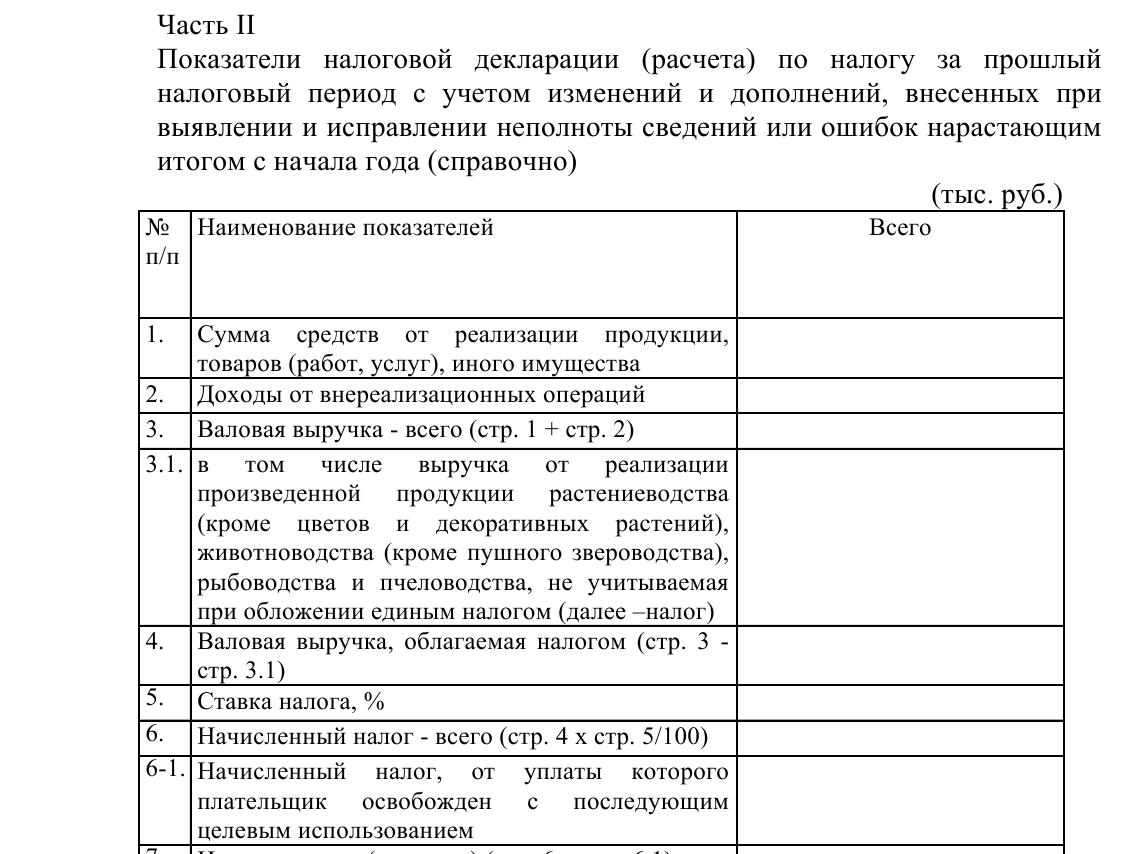
\includegraphics[scale=0.4]{pics/taxformrb}
  \caption{Фрагмент налоговой декларации}
  \label{pic:taxformrb}
\end{figure}


Налоговая декларация содержит различные данные о финансовой деятельности налогоплательщика. Процесс заполнения включает в себя процесс заполнения полей декларации. Существуют поля которые должны содержать информацию о финансовой деятельности налогоплательщика, поля которые представляют собой сумму каких-либо других полей декларации, поля, которые отображают отчетный период.

Заполнение налоговых деклараций на крупных предприятиях требует больших вычислений, которые связаны с учетом всей финансовой деятельности предприятия в отчетный период.
\section{Обзор существующих систем документооборота}
Рассмотрим существующие системы документооборота, которые позволяют автоматизировать процесс налоговой отчетности.
\subsection{Программный продукт 1C Бухгалтерия}
Программный продукт "1С:Бухгалтерия" — универсальная программа массового назначения для автоматизации бухгалтерского и налогового учета, включая подготовку обязательной (регламентированной) отчетности. Это готовое решение для ведения учета в организациях, осуществляющих любые виды коммерческой деятельности: оптовую и розничную торговлю, комиссионную торговлю (в том числе субкомиссию), оказание услуг, производство и т.д. Кроме того, с помощью ``1С:Бухгалтерии" могут вести учет индивидуальные предприниматели, применяющие упрощенную систему налогообложения или общий режим налогообложения.
\parБухгалтерский и налоговый учет реализованы в соответствии с действующим законодательством Российской Федерации. В состав конфигурации включен план счетов бухгалтерского учета, настроенный в соответствии с Приказом Минфина РФ "Об утверждении плана счетов бухгалтерского учета финансово-хозяйственной деятельности организаций и инструкции по его применению" от 31 октября 2000 г. № 94н.
\parМетодика бухгалтерского учета обеспечивает одновременную регистрацию каждой записи хозяйственной операции как по счетам бухгалтерского учета, так и по необходимым разрезам аналитического учета, количественного и валютного учета. Пользователи могут самостоятельно управлять методикой учета в рамках настройки учетной политики, создавать новые субсчета и разрезы аналитического учета.
\parПредметная область, автоматизируемая "1С:Бухгалтерией" изображена на рисунке~\ref{pic:1c_image1}.
\begin{figure}
  \centering
  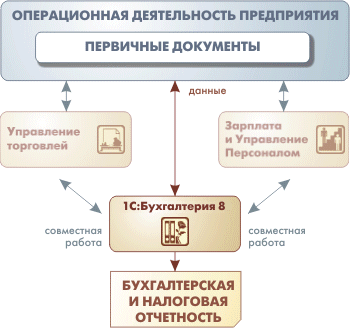
\includegraphics{pics/1c_image1}
  \caption{Предметная область, автоматизируемая ``1С:Бухгалтерией''}
  \label{pic:1c_image1}
\end{figure}
В подсистеме расчета заработной платы обеспечено формирование бумажной и электронной отчетности по налогам, связанным с заработной платой, в частности НДФЛ и ЕСН. Реализован персонифицированный учет взносов в Пенсионный фонд. Для расчета налогов и сборов и формирования налоговых деклараций используется регламентированная отчетность.
\begin{figure}
  \centering
  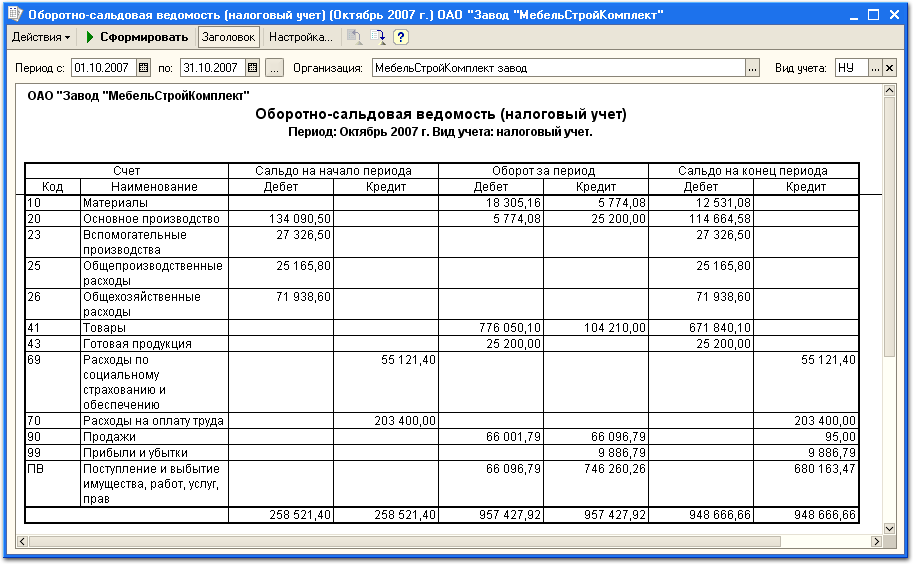
\includegraphics[scale=0.5]{pics/1c_image2}
  \caption{Окно для заполнения налогового декларации в системе 1С:Бухгалтерия}
  \label{pic:1c_image2}
\end{figure}
\subsection{Программный продукт Галактика ERP}
Автоматизированная система управления Галактика ERP (Enterprise Resource Planning) - это отечественная ERP-система для комплексной автоматизации бизнеса, основа комплекса Галактика Business Suite.
\parВозможности системы ERP позволяют в едином информационном пространстве оперативно решать главные управленческие задачи, обеспечить менеджеров различного уровня управления необходимой и достоверной информацией для принятия управленческих решений.
\parВ состав системы автоматизации управления предприятием Галактика ERP входят средства и для поддержки специальных управленческих задач:
\begin{itemize}
  \itemуправление техническим обслуживанием и ремонтами оборудования;
  \itemуправление качеством продукции;
  \itemуправление взаимоотношениями с клиентами;
  \itemуправление недвижимостью;
\end{itemize}
\parСистема состоит из нескольких функциональных блоков – контуров, каждый их которых решает комплекс задач: управление финансами, производством, логистикой, взаимоотношениями с клиентами и другие. Каждый контур состоит из нескольких модулей, нацеленных на выполнение более узких задач. Модульная структура Галактики ERP позволяет приобретать и использовать только те модули и контуры, которые необходимы конкретному предприятию. С развитием бизнеса и появлением новых управленческих задач, предприятие имеет возможность последовательно производить закупку необходимых компонент системы.
\parВ системе Галактика ERP реализована концепция компонентной модели: все единицы системы сформированы в компоненты, взаимодействующие между собой через специальные интерфейсы. Компоненты логически объединены в модули системы Галактика ERP. Наличие версий у компонентов позволяет перейти от обновления системы к обновлению отдельных компонентов.
\parСистема Галактика ERP поддерживает русский, белорусский, украинский и казахский языки.
\parВ состав системы Галактика ERP включены средства для централизованной настройки параметров системы, ее обновления, установки необходимых приложений. Это существенно повышает безопасность системы, улучшает защиту от несанкционированного доступа и значительно облегчает процесс ее администрирования.
Для автоматизированного учета налогов в системе Галактика ERP реализованы гибкие и универсальные механизмы, позволяющие оперативно ``подстраиваться'' под изменяющееся законодательство. Система дает возможность раздельного ведения бухгалтерского и налогового учета, формирования налоговых регистров и налоговой отчетности в соответствии с требованиями действующего налогового законодательства.
Принцип построения налогового учета в системе базируется на однократной регистрации первичных документов, формировании учетных записей от первичного документа с использованием настроенных типовых хозяйственных операций, использовании набора готовых деклараций и механизма настройки, а также создании пользовательских отчетных форм для расширения состава деклараций в соответствии с требованиями предприятия. Налоговая отчетность строится на данных первичных документов и сформированных по ним проводок. Для налогового учета можно использовать как параллельный план счетов, так и бухгалтерский план счетов, расширенный специально введенными для налогового учета синтетическими и аналитическими разрезами учета.
\parСредства системы Галактика ERP по ведению налогового учета сосредоточены не только в модуле Налоговый учет, но и в других модулях системы. В модуле Налоговый учет скомпонованы основные функциональные средства по документированию налогооблагаемой базы по налогу на прибыль. Он содержит специально разработанную систему интерактивных настраиваемых деклараций для формирования налоговых регистров. Функции для формирования регистров сгруппированы по типам операций. Каждый полученный в результате регистр отражает перечень показателей, на основе которых можно осуществить исчисление налоговой базы.
\subsection{Программный продукт Парус}
Программные продукты ``ПАРУС'' (ПП ``ПАРУС'') — предназначены для автоматизации деятельности коммерческих предприятий и бюджетных учреждений разного уровня. Среди линеек ПП ``ПАРУС'' есть и тиражные продукты и относящиеся к классу ERP-систем.
\parСистема строится на базе двухзвенной архитектуры клиент-сервер с использованием СУДБ Oracle(рисунок~\ref{pic:parus_pic1}).
\begin{figure}
  \centering
  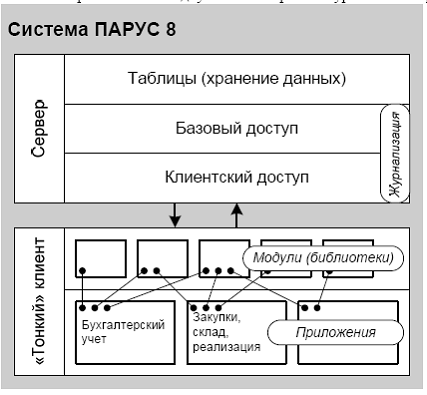
\includegraphics[scale=0.7]{pics/parus_img1}
  \caption{Двухзвенная архитектура системы ``ПАРУС''}
  \label{pic:parus_pic1}
\end{figure}
На сервере размещаются уровни:
\begin{itemize}
\itemхранения данных;
\itemбазового доступа: реализуются алгоритмы простейших бизнес-процедур;
\itemклиентского доступа: реализуются процедуры, составленные из одного или нескольких элементов базового доступа, – с поддержкой управления правами доступа пользователей и пользовательских настроек;
\end{itemize}
Возможные конфигурации построения:
\begin{itemize}
  \itemоднопользовательская;
  \itemлокальная сеть;
  \item WEB-решения;
  \itemтерминальный доступ;
\end{itemize}
Модуль ``Бухгалтерский учет'' предназначен для автоматизации ведения бухгалтерского учета в бюджетных учреждениях любого уровня. В модуле реализован документооборот всех участков бухгалтерского учета, которые ведут главные распорядители, распорядители и получатели бюджетных средств, в соответствии с положениями действующих нормативных документов.
В модуле реализованы учетные регистры для учета всех видов первичных документов и учетной информации, ведение которых предусмотрено нормативными документами, регулирующими ведение бухгалтерского учета. Модуль имеет интуитивно понятный интерфейс, все функциональные возможности сгруппированы по принципу принадлежности к участкам бухгалтерского учета. Благодаря широкому набору функциональных возможностей модуль позволяет полностью автоматизировать:
\begin{enumerate}
  \itemучет операций по санкционированию расходования бюджетных средств;
  \itemучет финансовых активов (операций с денежными средствами);
  \itemэлектронное взаимодействие с отделениями Федерального казначейства;
  \itemучет расчетов с поставщиками и подрядчиками;
  \itemучет нефинансовых активов;
\end{enumerate}
Упрощённая схема модуля ``Бухгалтерский учет'' и его взаимодействие с другими модулями представлено на рисунке~\ref{pic:parus_pic2}
\begin{figure}
  \centering
  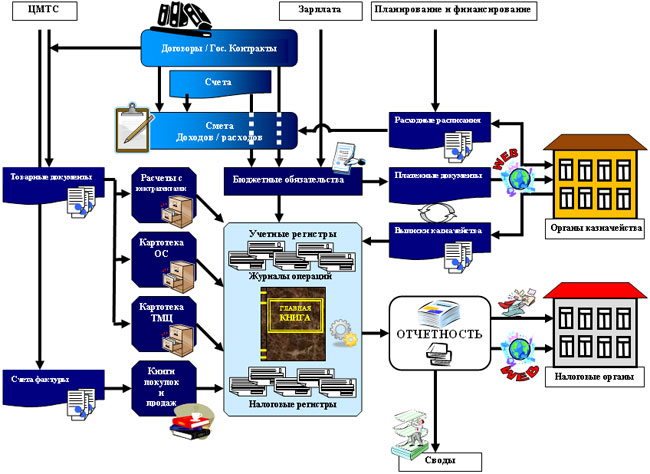
\includegraphics[scale=0.6]{pics/parus_img2}
  \caption{Упрощённая схема модуля ``Бухгалтерский учет''}
  \label{pic:parus_pic2}
\end{figure}
\subsection{Программный продукт Microsoft Dynamics NAV}
Программный продукт Microsoft Dynamics NAV — интегрированная система управления предприятием  класса ERP, поставляемая корпорацией Microsoft в новой линейке продуктов Microsoft Dynamics для среднего и малого бизнеса. В этой системе реализована следующая функциональность:
\begin{itemize}
  \itemуправление финансами;
  \itemбизнес-анализ;
  \itemуправление цепочками поставок;
  \itemуправление складом;
  \itemуправление отношениями с клиентами;
  \itemэлектронная коммерция;
  \itemпроизводство;
\end{itemize}
\parФинансовый контур системы Microsoft Dynamics NAV полностью интегрирован с функциональностью управления складом и производством, а также с блоками расчетов с клиентами и поставщиками, учета основных средств, заработной платы. Это позволяет автоматически и в режиме реального времени отражать на финансовых счетах главной книги себестоимость товаров, произведенной продукции и оказанных услуг, а также скидки, издержки, накладные расходы, начисление НДС и прочие данные. Уникальная технология индексного суммирования позволяет мгновенно обновлять итоговые суммы после проведения транзакции любой сложности. Благодаря этому можно в режиме реального времени получить показатели за любой период и с любым количеством установленных фильтров.
\par Microsoft Dynamics NAV позволяет автоматически создавать корпоративную отчетность любой степени детализации и сложности. Отчетность формируется независимо от планов счетов, количества анализируемых показателей, валюты и продолжительности учетных периодов фирм-филиалов. Многовалютность системы позволяет вести баланс в рублях и в дополнительной отчетной валюте. При этом полностью сохраняется история операций с точки зрения оригинальной валюты.
\par Microsoft Dynamics NAV отличается мощными средствами трассировки и контроля источников происхождения любой операции, что делает прозрачными и доступными для понимания самые сложные транзакции. В системе автоматически формируются учетные финансовые регистры. Уникальная функция ``Навигатор'' позволяет на основании даты и номера документа выявить все взаимосвязанные операции и документы, выяснить дату построения транзакции и идентифицировать создавшего ее пользователя.
\par Microsoft Dynamics NAV отличается гибкостью настройки бизнес-правил и процедур учета, возможностями модификации стандартных форм и деклараций. Это позволяет вам легко и быстро адаптировать систему к любым изменениям в бизнесе, самостоятельно расширяя детализацию аналитики и тем самым создавая ваше собственное информационное решение.
\par Microsoft Dynamics NAV содержит средства бюджетирования, планирования и мониторинга бюджетов. Бюджетная система компании может включать любое количество бюджетов с разной степенью детализации – от подразделений до сводных бюджетов всего холдинга. Аналитические измерения позволяют создавать бюджеты по индивидуальным статьям затрат и доходов. Система матричных форм бюджетов предназначена как для мониторинга деятельности отдельных подразделений компании, так и для сравнения с показателями любых предыдущих периодов.
\parДля дополнительного удобства и гибкости работы с бюджетами в Microsoft Dynamics NAV предусмотрена интеграция с Microsoft Office Excel, которая позволяет импортировать и экспортировать бюджетные показатели.
Межфирменный учет упрощает и оптимизирует бизнес-процессы и транзакции, проводимые между всеми структурными единицами бизнеса, имеющими отдельный баланс. Внедрение этого модуля позволяет эффективно управлять дочерними и внутренними организациями-партнерами, филиалами и аффилированными компаниями, в том числе находящимися в других странах.
\parРабочая среда Microsoft Dynamics NAV позволяет рассылать документы о продажах и покупках и распространять операции финансового журнала на все подчиненные офисы, коммерческие отделы или дочерние компании, что упрощает документооборот и снижает трудозатраты. Информация о межфирменной транзакции вводится в соответствующие документы только один раз.
\parПользователи полностью контролируют все документы, связанные с транзакциями. Например, они могут отклонить присланный им документ и таким образом аннулировать неверные проводки. Осуществляя закупку у компании-партнера или дочерней фирмы, они могут корректировать заказ, пока не начнется отгрузка товара.
\parДля формирования бухгалтерской и налоговой отчетности реализован механизм, позволяющий заполнять отчетные формы на основании данных по финансовым счетам, операциям с НДС и заработной плате сотрудников. При этом пользователь может самостоятельно, не прибегая к помощи специалиста, управлять механизмом формирования отчетности, динамически изменяя алгоритм расчета строк документов с учетом текущего изменения плана счетов и аналитики.
\parС помощью механизма регламентной отчетности можно выгружать данные из регламентных деклараций Microsoft Dynamics NAV в шаблоны файлов Microsoft Office Excel. Интеграция с Microsoft Office Excel позволяет хранить в базе данных Microsoft Dynamics NAV шаблоны выходных форм и экспортировать итоги вычислений в определенные ячейки файла-шаблона, что существенно повышает гибкость работы с результирующими формами и обеспечивает поддержку актуальности бухгалтерских форм.
\parВ декларации активно используются разнообразные фильтры и переменные параметры. В частности, в подмодуле ``Финансовые операции'' представлен перечень внутренней отчетности, необходимой в работе бухгалтера. Это журналы-ордера, оборотные ведомости, ``шахматки'', бухгалтерские карточки счетов, поставщиков, клиентов и банков, анализ счета и т.д. Помимо бухгалтерских деклараций внутреннего пользования Microsoft Dynamics NAV содержит большой набор унифицированных форм документов по учету основных средств, кассовых и банковских операций, складские, товарно-отгрузочные документы и т.д. При необходимости любой отчет может быть модифицирован и адаптирован применительно к специфике деятельности предприятия.
\parОдин из основных участков ведения учета – учет кассовых и банковских операций. В Microsoft Dynamics NAV реализован весь спектр кассовых операций. Подмодуль ``Денежные средства'' модуля ``Финансы'' позволяет заносить и учитывать приходные и расходные ордеры на клиентов, поставщиков и подотчетных лиц, на банковские счета и напрямую на финансовый счет. Реализованы все декларации, необходимые для ведения кассовых операций:
\begin{itemize}
  \itemприходный кассовый ордер;
  \itemрасходный кассовый ордер;
  \itemкассовая книга;
  \itemжурнал регистрации приходных и расходных ордеров;
\end{itemize}
\parКаждая компания может вести неограниченное количество расчетных счетов в любой валюте. Система хранит полную историю проведения платежей, включая формирование платежного документа, внесение изменений в документ, отмену документа, повторное создание документа и т.д.
\begin{figure}
  \centering
  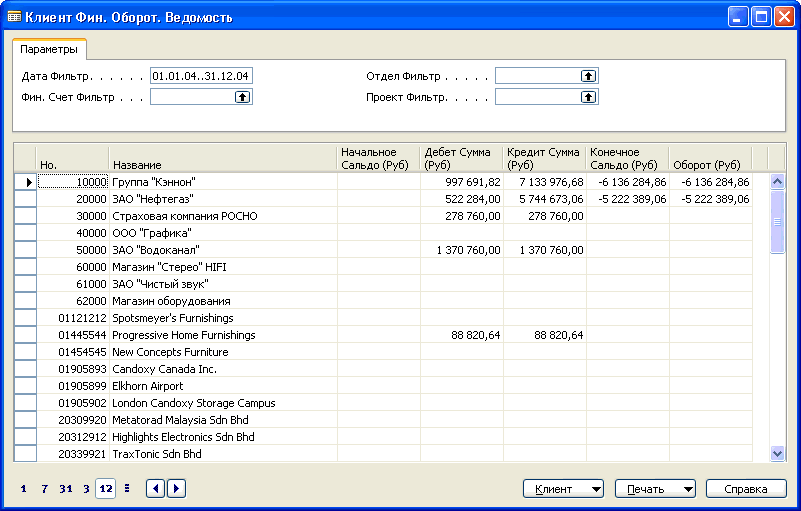
\includegraphics[scale=0.50]{pics/navision_img1}
  \caption{Оборотная ведомость в разрезе клиентов}
  \label{pic:navision_pic1}
\end{figure}

\subsection{Сравнение систем документооборота}
Проведем сравнение рассмотренных систем документооборота. Сравнение будем производить по следующим критериям:
\begin{itemize}
  \itemТип - тип системы документооборота, который показывает предметную область в управлении предприятием (которая может включать в себя не только финансовую деятельность) которую автоматизирует система;
  \itemОС - поддерживаемые операционные системы;
  \itemСтруктура - структура приложения, которую представляет собой рассматриваемая система;
  \itemБаза данных - тип базы данных, которая используется для хранения информации;
  \itemЛицензия - лицензия, под которой распространяется система;
\end{itemize}
Результаты сравнения приведены в таблицах~\ref{tabl:analys_1} и ~\ref{tabl:analys_2}
\begin{table}
  \centering
  \caption{Результат сравнения систем документооборота(Начало)}
  \label{tabl:analys_1}
\begin{tabular}{|m{3.2cm}|m{3cm}|m{2cm}|m{2.5cm}|m{4cm}|}
  \hline
  \bfseries{Название системы} &
  \bfseries{Тип} &
  \bfseries{ОС} &
  \bfseries{Структура} &
  \bfseries{База Данных}\\
  \hline
  1C Бухгалтерия & Система бухгалтерского учета & Windows, GNU Linux & Standalone, Web & 1CD(собственный формат), Microsoft SQL Server, DBF\\
  \hline
  Галлактика ERP & Система планирования ресурсов предприятия & Windows  & Standalone  & PervasiveSQL, Microsoft SQL Server, Oracle\\
  \hline
  Парус & Система планирования ресурсов предприятия & Windows & Standalone, Web & Oracle\\
  \hline
  Microsoft Dynamic NAV & Система планирования ресурсов предприятия & Windows & Standalone, Web & Microsoft SQL Server\\
  \hline
\end{tabular}
\end{table}
\begin{table}
  \centering
  \caption{Результат сравнения систем документооборота(Продолжение)}
  \label{tabl:analys_2}
\begin{tabular}{|m{6cm}|m{4cm}|}
  \hline
  \bfseries{Название системы} &
  \bfseries{Лицензия}\\
  \hline
  1C Бухгалтерия & Коммерческая\\
  \hline
  Галлактика ERP & Коммерческая\\
  \hline
  Парус & Коммерческая\\
  \hline
  Microsoft Dynamic NAV & Коммерческая\\
  \hline
\end{tabular}
\end{table}

\chapter{Проектирование системы создания и управления электронными налоговыми декларациями}

\section{Требования, предъявляемые к системе}
В качестве исходных данных были предъявлены следующие требования к разрабатываемой системе:
\begin{enumerate}
  \itemСистема должна обеспечить разграничение прав. Система должна поддерживать работу пользователей, каждый пользователь может иметь свои настройки. Группа пользователей объединяется в домен, в каждом домене есть администратор, который может добавлять, удалять пользователей, либо изменять настройки каждого пользователя из домена.
  \itemСистема должна предоставлять web интерфейс. Для работы с системой пользователь должен иметь возможность использовать web-интерфейс, что позволяет использовать систему практически из любого окружение, для доступа к системе нужен только веб-браузер.
  \itemДля хранения данных должна использоваться реляционная база данных. Данные о заполненных декларациях должны храниться в реляционной базе данных.
  \itemТребуется обеспечить возможность добавление новых деклараций и изменения существующих. декларации могут изменяться (добавляться, удаляться, изменяться содержимое) в каждом налоговом году, для этого необходимо предоставить простой способ для достижения этой цели.
  \itemТребуется предоставить возможность изменения правил подсчета для ячеек деклараций. Ячейки, которые считаются по формулам, либо по каким-то другим правилам могут быть переписаны произвольным значением, которые задаст пользователь.
\end{enumerate}

\section{Анализ требований}
Проведем анализ предъявленных требований:
\begin{enumerate}
  \itemТребуется ввести сущность Пользователь и Домен. Все сущности, которые будут создаваться пользователями в системе не будут доступны для пользователей из других доменов, так же можно ограничить доступ к создаваемым сущностям для пользователей одного домена. Пользователь будет однозначно идентифицироваться доменом, именем. Для входа в систему пользователю необходимо ввести пароль.
  \itemСистема будет представлять собой клиент-серверное приложение, в котором клиентом будет выступать браузер(иногда называется ``тонким клиентом''), а сервером - веб-сервер. Логика веб-приложения распределена между сервером и клиентом, хранение данных будет осуществляться на сервере, обмен данными будет происходить по сети. Возможность обновления и поддержки веб-приложений без установки дополнительного программного обеспечения у клиента является одной из ключевых причин популярности веб приложений.
  \itemВся информация о сущностях, созданных пользователями будет храниться в реляционной базе данных. Реляционная база данных - база данных, основанная на реляционной модели данных. Реляционная модель данных основана на математическом понятии отношение (relation). Для работы с реляционными базами данных применяются реляционные Системы Управления Базами Данных (СУБД). Наиболее известные реляционные СУБД: MySQL, Oracle, Postgres. Для создания, модификации и управления данными обычно используется язык Structured Query Language (SQL).
  \itemДля обеспечения добавления новых деклараций и изменения старых необходимо выделить структуры для представления деклараций и физическое представление этих структур. Для представления деклараций будет использоваться язык XML, каждый отчет будет описан с использованием данного языка. XML (eXtensible Markup Language) — рекомендованный Консорциумом Всемирной паутины язык разметки, фактически представляющий собой свод общих синтаксических правил. XML — текстовый формат, предназначенный для хранения структурированных данных , для обмена информацией между программами, а также для создания на его основе более специализированных языков разметки (например, XHTML), иногда называемых словарями.
\begin{figure}
  \centering
  \begin{small}
    \begin{verbatim}
      <instructions>
         <step>Смешать</step>
         <step>Закрыть</step>
         <step>Замесить</step>
      </instructions>
    \end{verbatim}
  \end{small}
  \caption{Пример XML документа}
  \label{pic:xml_sample}
\end{figure}
%  \item PDF (Portable Document Format) — кроссплатформенный формат электронных документов, созданный фирмой Adobe Systems с использованием ряда возможностей языка PostScript. В первую очередь предназначен для представления в электронном виде полиграфической продукции, значительное количество современного профессионального печатного оборудования мо%жет обрабатывать PDF непосредственно. Для создания PDF документов в языке Java можно ис%пользовать библиотеку iText.
  \item Для выполнения данного требования необходимо выделить сущность, которая будет представлять тип подсчета для ячейки.
\end{enumerate}

\section{Объектная модель системы}
При проектирования системы будем использовать объектный подход.\\
В соответствии с предъявленными требованиями к системе, выделим объекты и определим связи между ними, представим результат в виде диаграммы сущность-связь (рисунок~\ref{pic:er_diagram}).

``Пользователь'' представляет собой пользователя системы, содержит атрибуты ``Имя'' - имя пользователя в системе, и ``Пароль'',  данные атрибуты однозначно определяют пользователя системы. ``Пользователь'' может создавать ``Компании'', каждая компания имеет уникальное ``Название'' в рамках одного ``Домена''. ``Бухгалтерская книга'' содержит информацию о состоянии баланса, которое представлено ``Счетами'' каждый счет имеет ``Номер'', значения ``Кредита'' и ``Дебета'', в рамках одной компании ``Бухгалтерская книга'' должна иметь уникальное ``Название''. ``Налоговые формы'' представляют собой набор экземпляров деклараций за определенный ``Год'', в рамках одной ``Компании'' ``Налоговые формы'' определяются ``Названием'' и ``Годом''. ``Декларация'' представляет собой налоговую декларацию, содержит набор ``Ячеек''. ``Ячейка'' определяется ``Названием'', каждая ячейка имеет ``Состояние'', сущность, которая определяет значение ячейки и её ``Тип'', ``Ячейка'' может быть нескольких типов, каждый тип определяет правила для подсчета ``Значения'' ячейки:

\begin{itemize}
  \item''Пользовательская'' - значение ячейки задает пользователь (атрибут ``Пользовательское значение'');
  \item''Счета'' - значение ячейки подсчитывается на основании списка ``Интервалов''. ``Интервал'' представляет собой интервал, в в котором содержатся ``Счета'' из ``Бухгалтерской книги'' для ``Налоговых форм'', которым принадлежит декларация. При подсчете данного типа ячейки используется сумма из значений ``Интервалов'', для каждого ``Интервала'' выбираются значения из ``Счетов'', номера которых находятся между значениями атрибутов ``От'' и ``До'', значения ``Счета'' (``Дебет'' либо ``Кредит'') выбираются в зависимости от атрибута ``Тип'';
  \item''Формула'' - значение ячейки считается согласно некоторому выражению, которое может содержать переменные, в качестве значений которых подставляются значения некоторых ячеек из текущей декларации. Например: \{A1\}+\{A2\}/100, значения переменных \{A1\} и \{A2\} будут равны значениям ячеек с именами \{A1\} и \{A2\} соответственно;
\end{itemize}

Для подсчета ``Декларации'' используется ``Калькулятор декларации'', сущность которая подсчитывает значения для ``Декларации'', используя ``Калькулятор ячейки'' для подсчета каждой ячейки в зависимости от её ``Типа''.

\begin{sidewaysfigure}
  \centering
  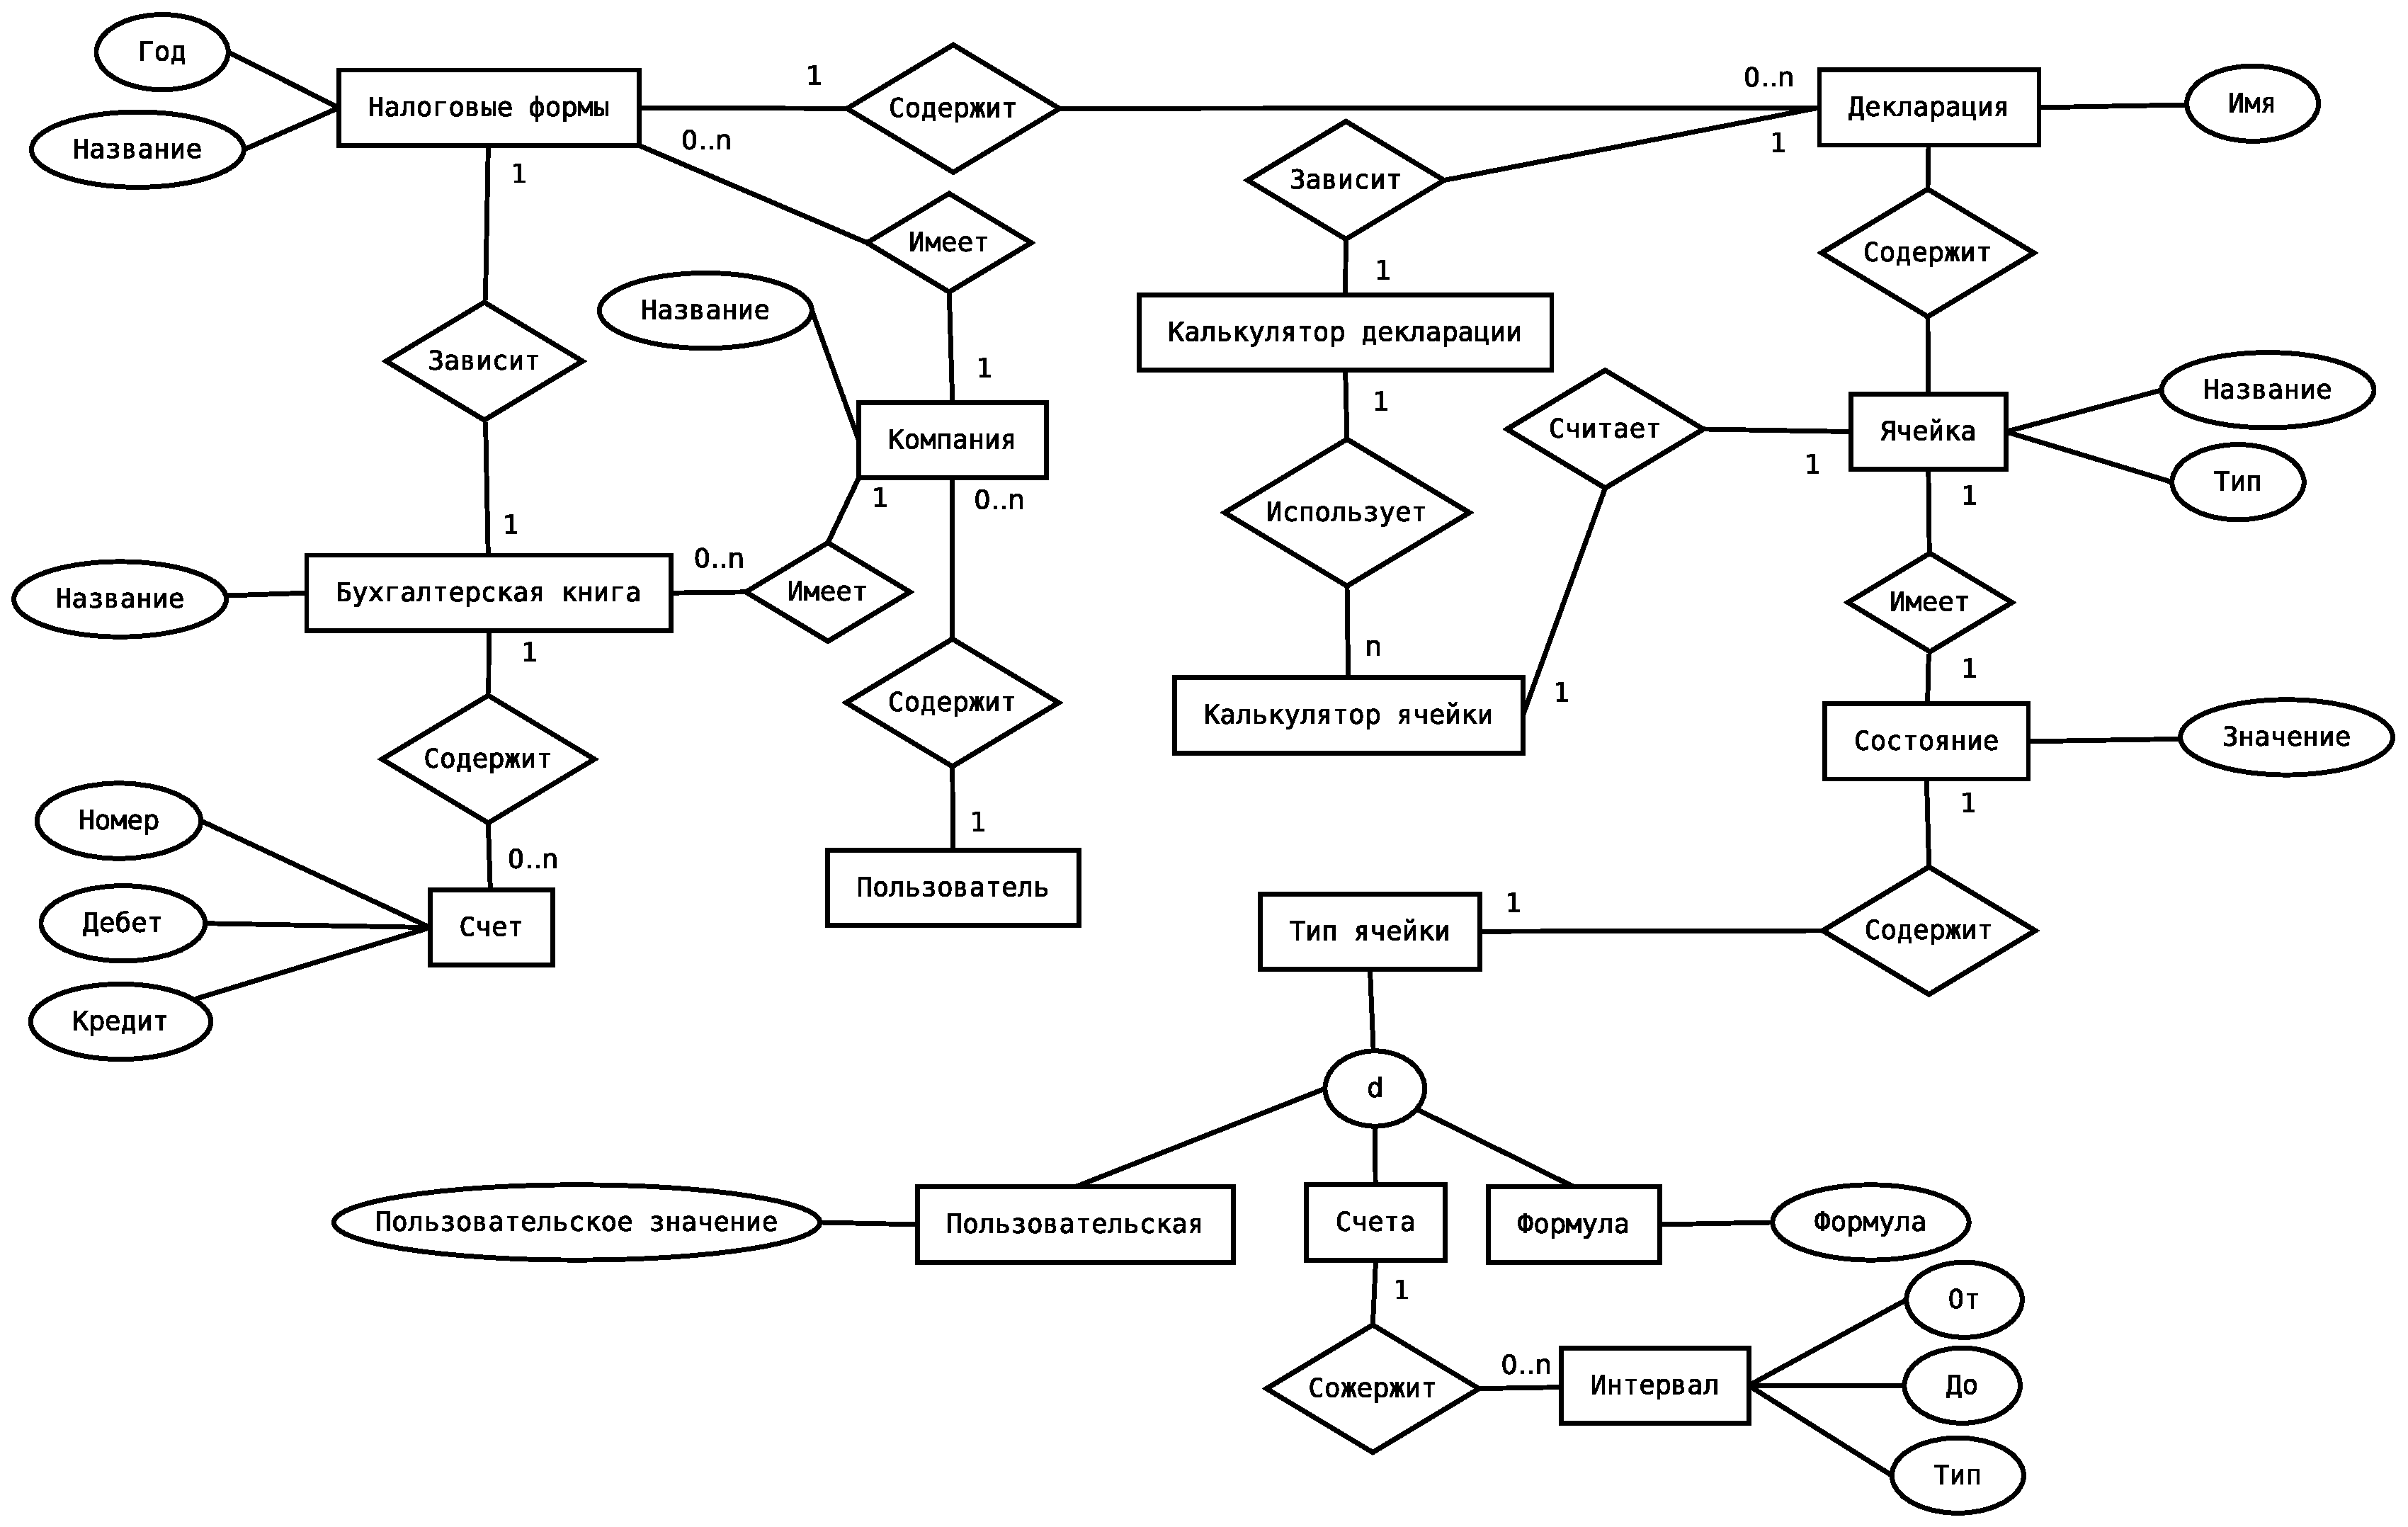
\includegraphics[scale=0.4]{uml/entity_pretty}
  \caption{Диаграмма сущность-связь}
  \label{pic:er_diagram}
\end{sidewaysfigure}

Отразим взаимодействие пользователя с сущностями системы на диаграммах вариантов использования. Пользователем системы будет являться человек, занимающий должность в организации, ответственную за заполнение налоговых деклараций и ведение бухгалтерии, в общем случае - это бухгалтер, по этому в качестве первостепенного актора на диаграммах вариантов использования будем использовать ``Бухгалтера''.

Рассмотрим диаграмму вариантов использования для работы с ``Компанией''. Пользователь может создавать новую компанию, может редактировать и удалить существующую (рисунок~\ref{pic:use_case_4}).

На рисунке~\ref{pic:use_case_3} приведена диаграмма вариантов использования для работы с ``Бухгалтерской книгой'', пользователь может создавать ``Бухгалтерскую книгу'', может её редактировать, при редактировании возможно добавление, удаление и редактирования ``Счетов'', так же пользователь может удалить уже существующую ``Бухгалтерскую книгу''.

Изобразим варианты использования для работы с ``Набором деклараций'' (рисунок~\ref{pic:use_case_2}), пользователь может создать, редактировать и удалить уже существующий ``Набор деклараций''.

Рассмотрим варианты использования для работы ``Декларацией'' (рисунок~\ref{pic:use_case_1}). ``Бухгалтер'' является пользователем системы, ``Калькулятор декларации'' и ``Калькулятор ячейки'' - сущности системы, которые выполняют действия, необходимые для подсчета всей декларации и одной ячейки соответственно. ``Бухгалтер'' открывает декларацию, ``Калькулятор декларации'' подсчитывает открываемую декларацию. ``Бухгалтер'' может пересчитать значение ячейки, изменить тип значения ячейки - задать другой тип ячейки из возможных, либо изменить параметр ячейки, данные действия вызывают пересчет ячейки, за что отвечает ``Калькулятор ячейки''.

\begin{figure}
  \centering
  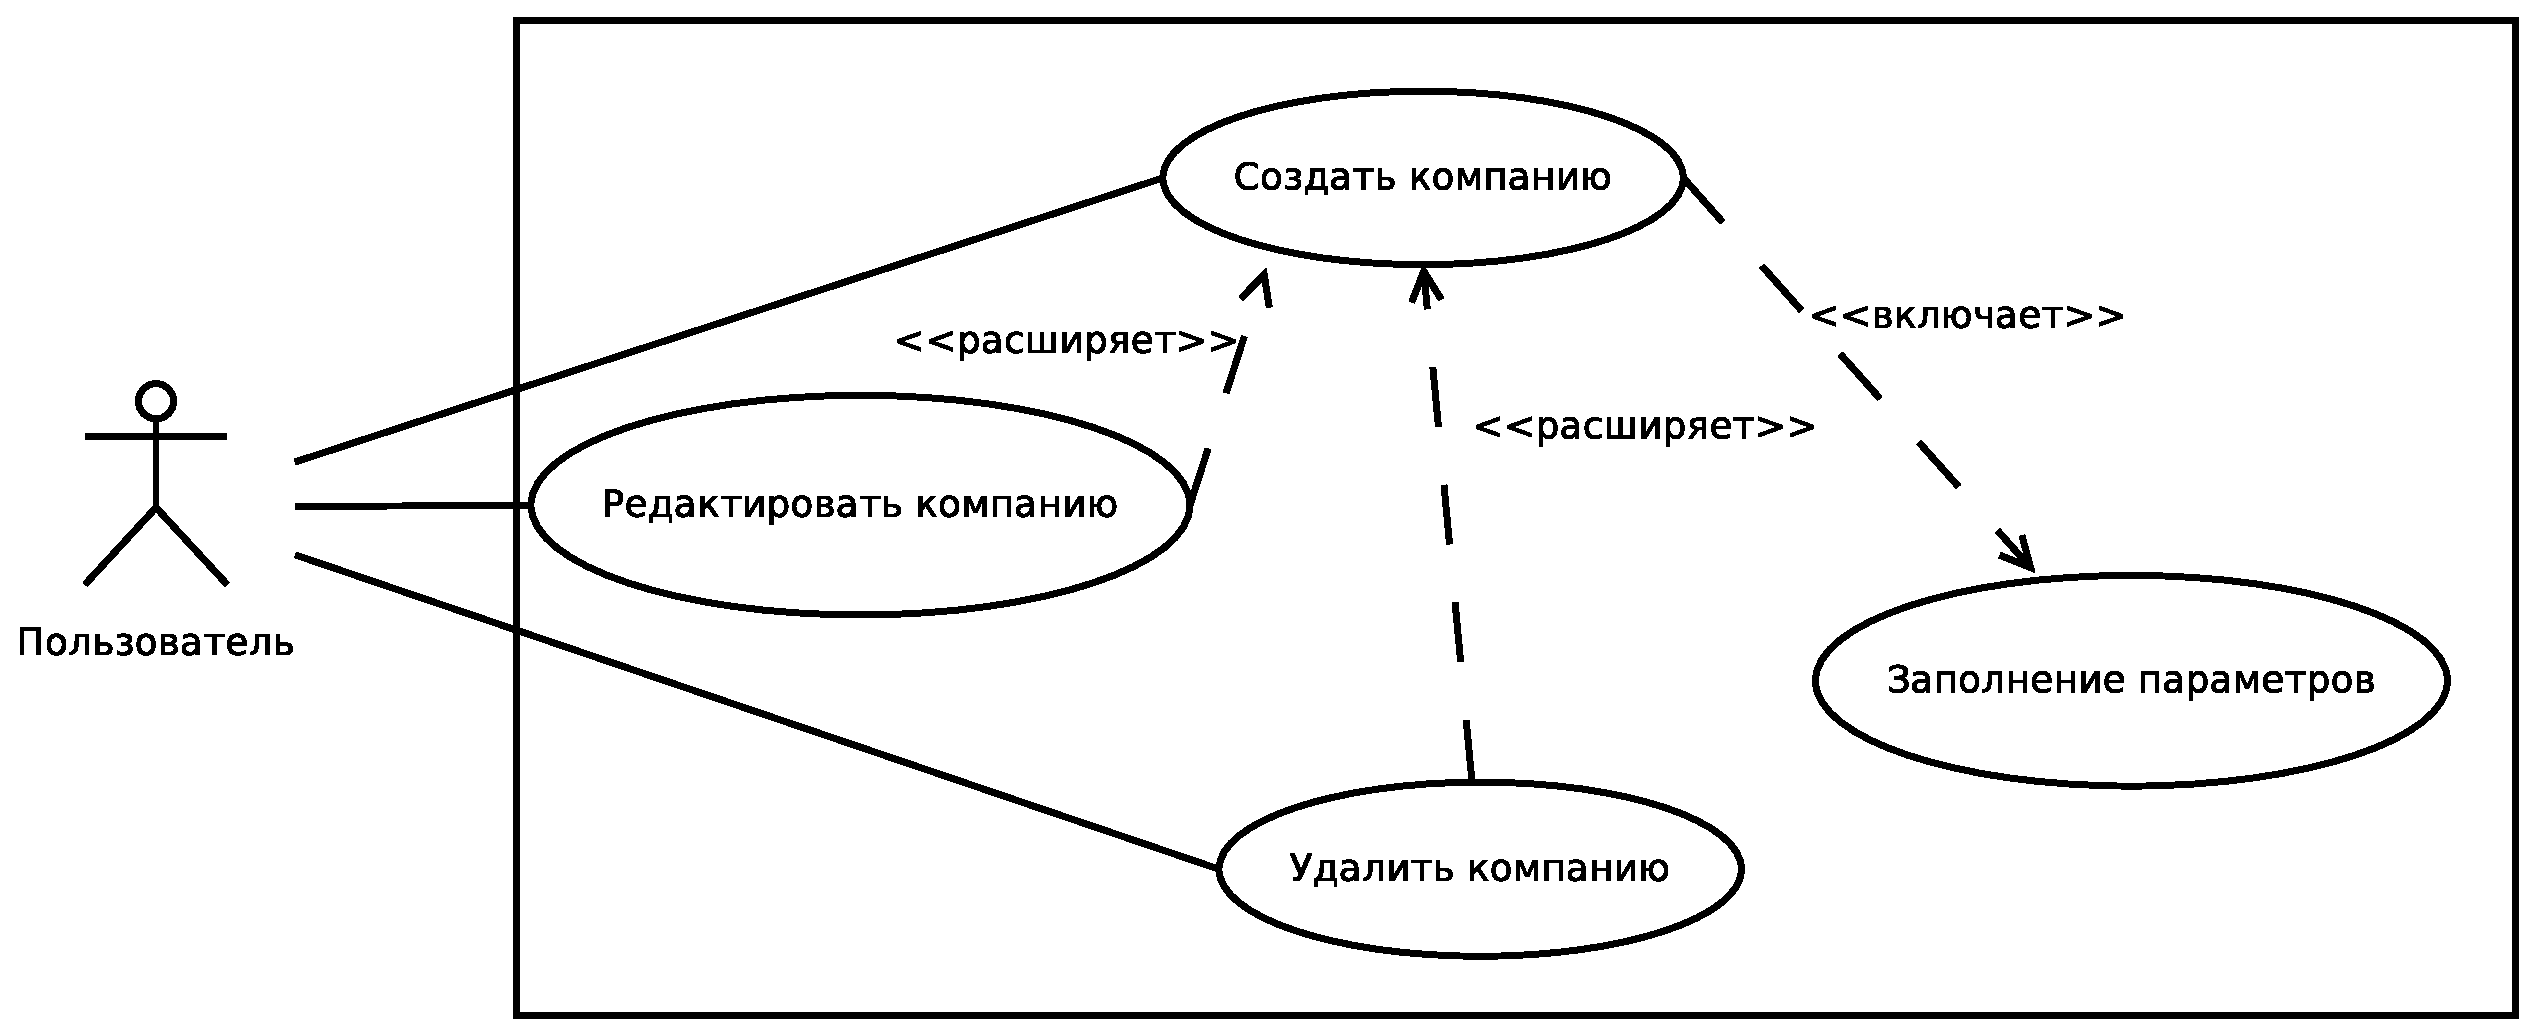
\includegraphics[scale=0.4]{uml/usecase_4}
  \caption{Диаграмма вариантов использования для работы с компанией}
  \label{pic:use_case_4}
\end{figure}

\begin{figure}
  \centering
  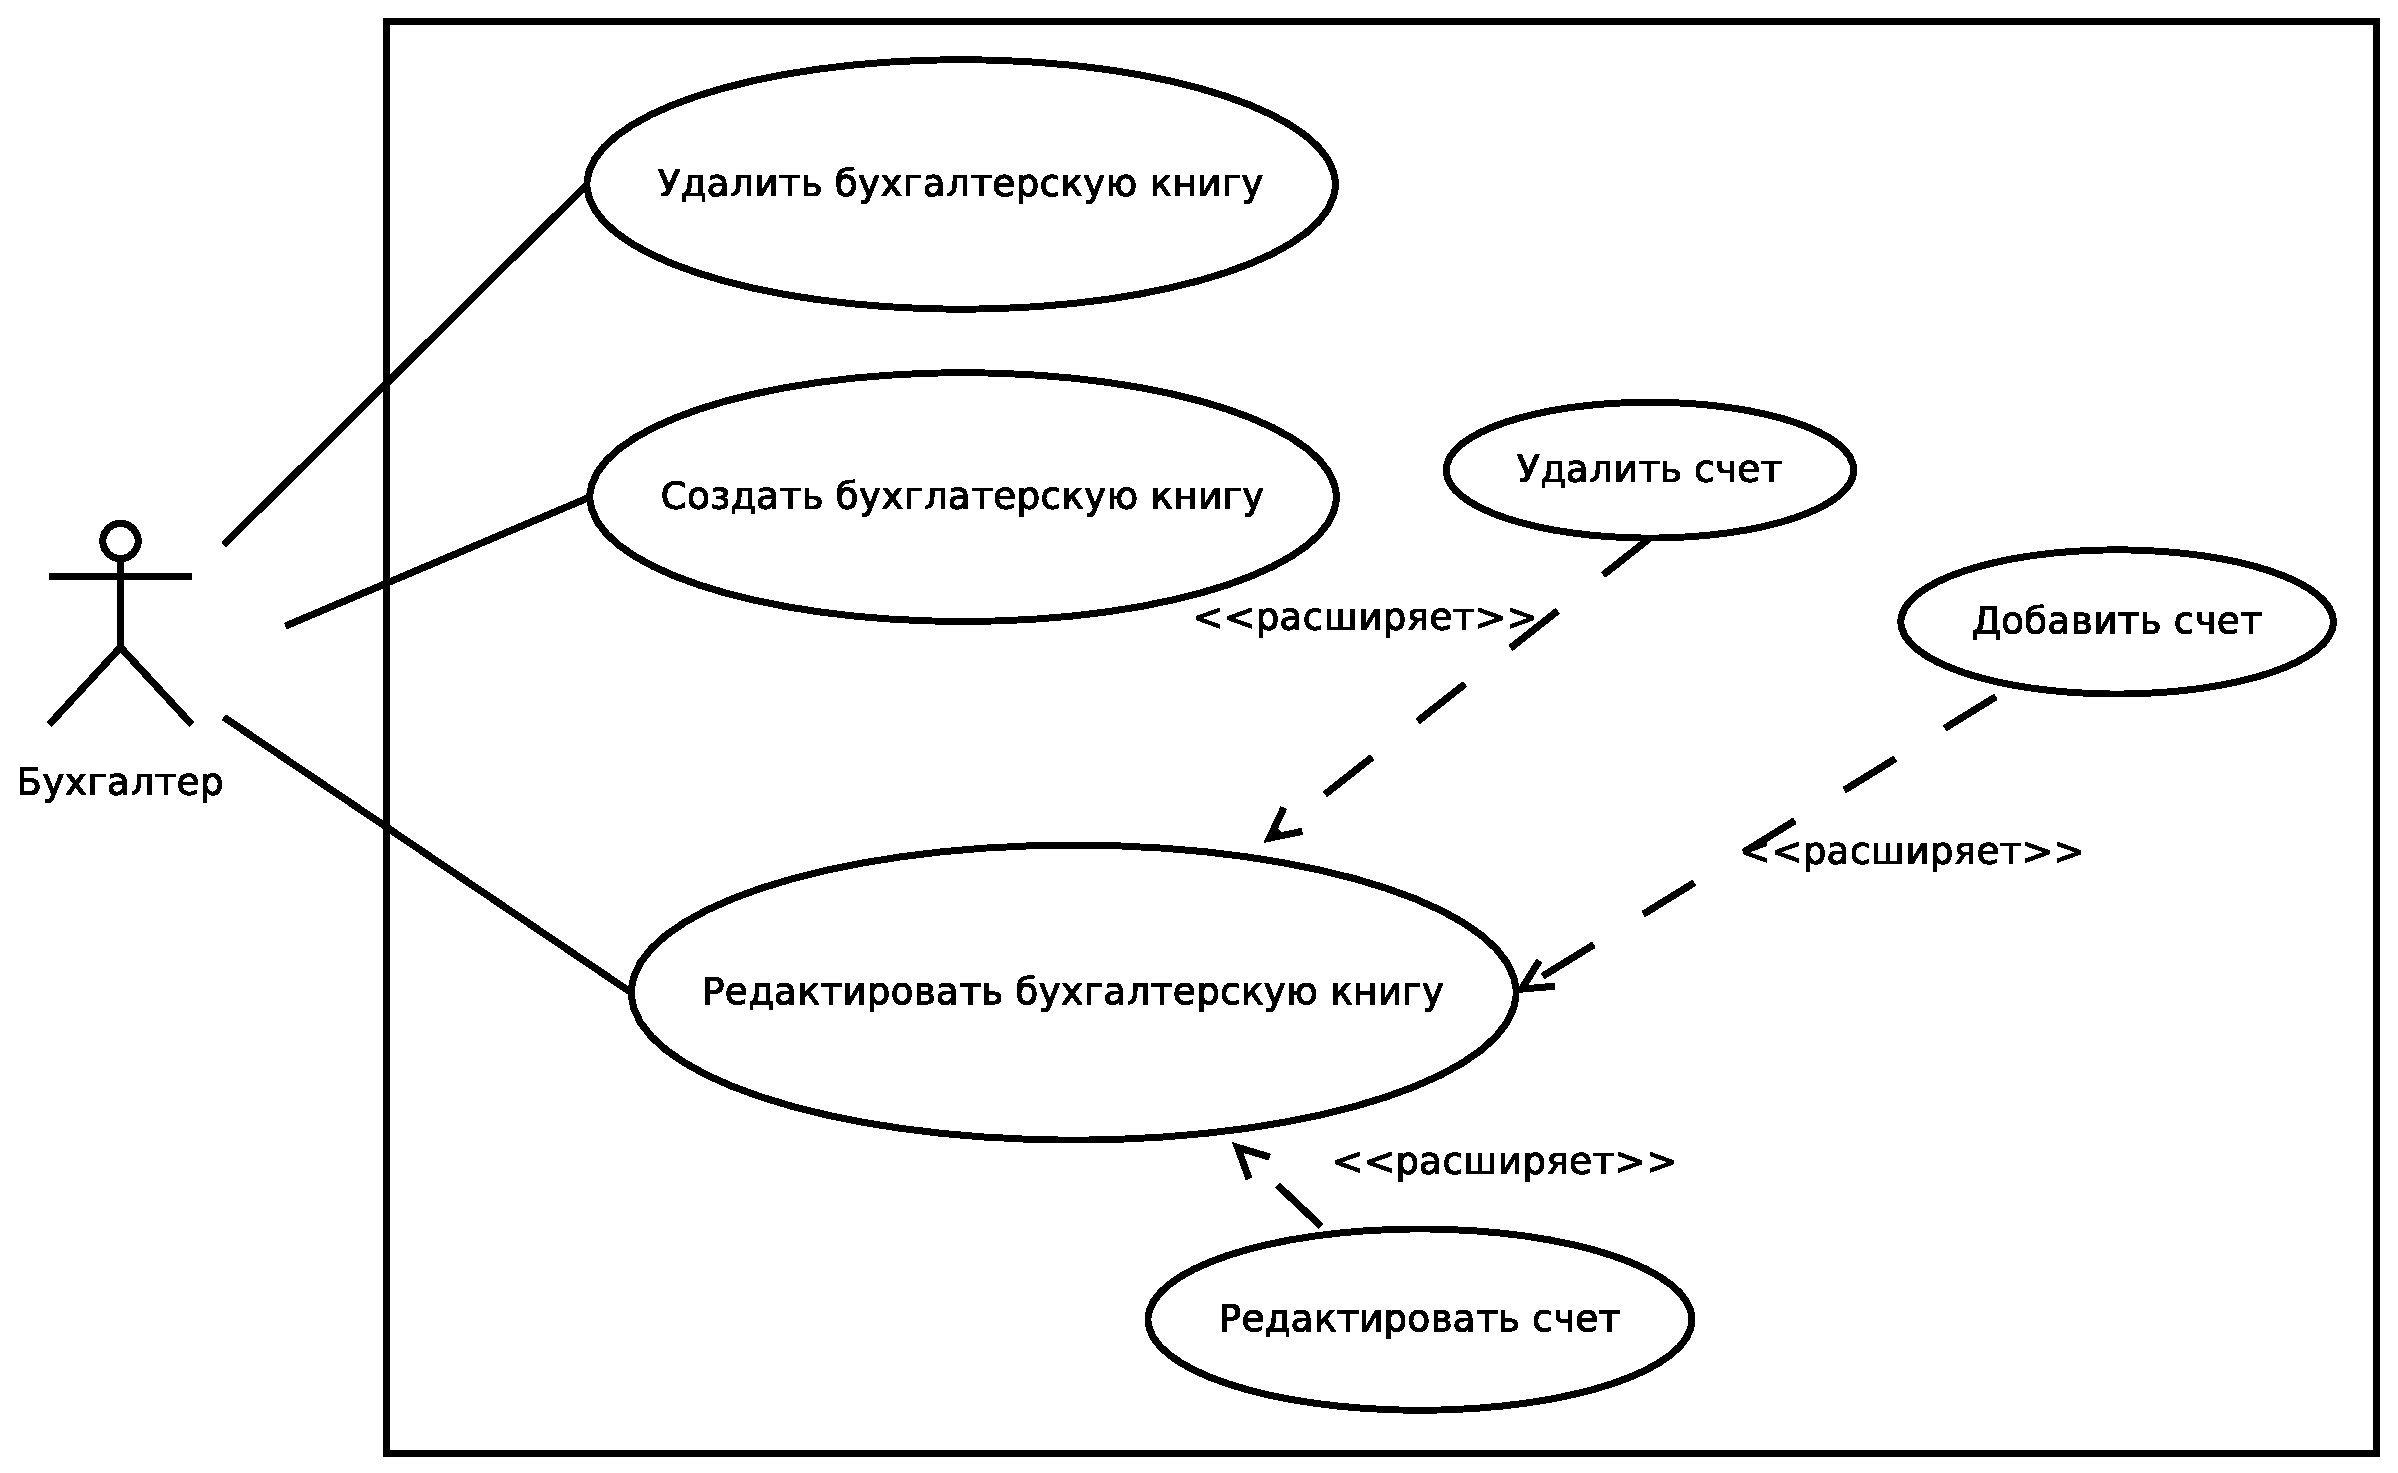
\includegraphics[scale=0.4]{uml/usecase_3}
  \caption{Диаграмма вариантов использования для работы с бухгалтерской книгой}
  \label{pic:use_case_3}
\end{figure}

\begin{figure}
  \centering
  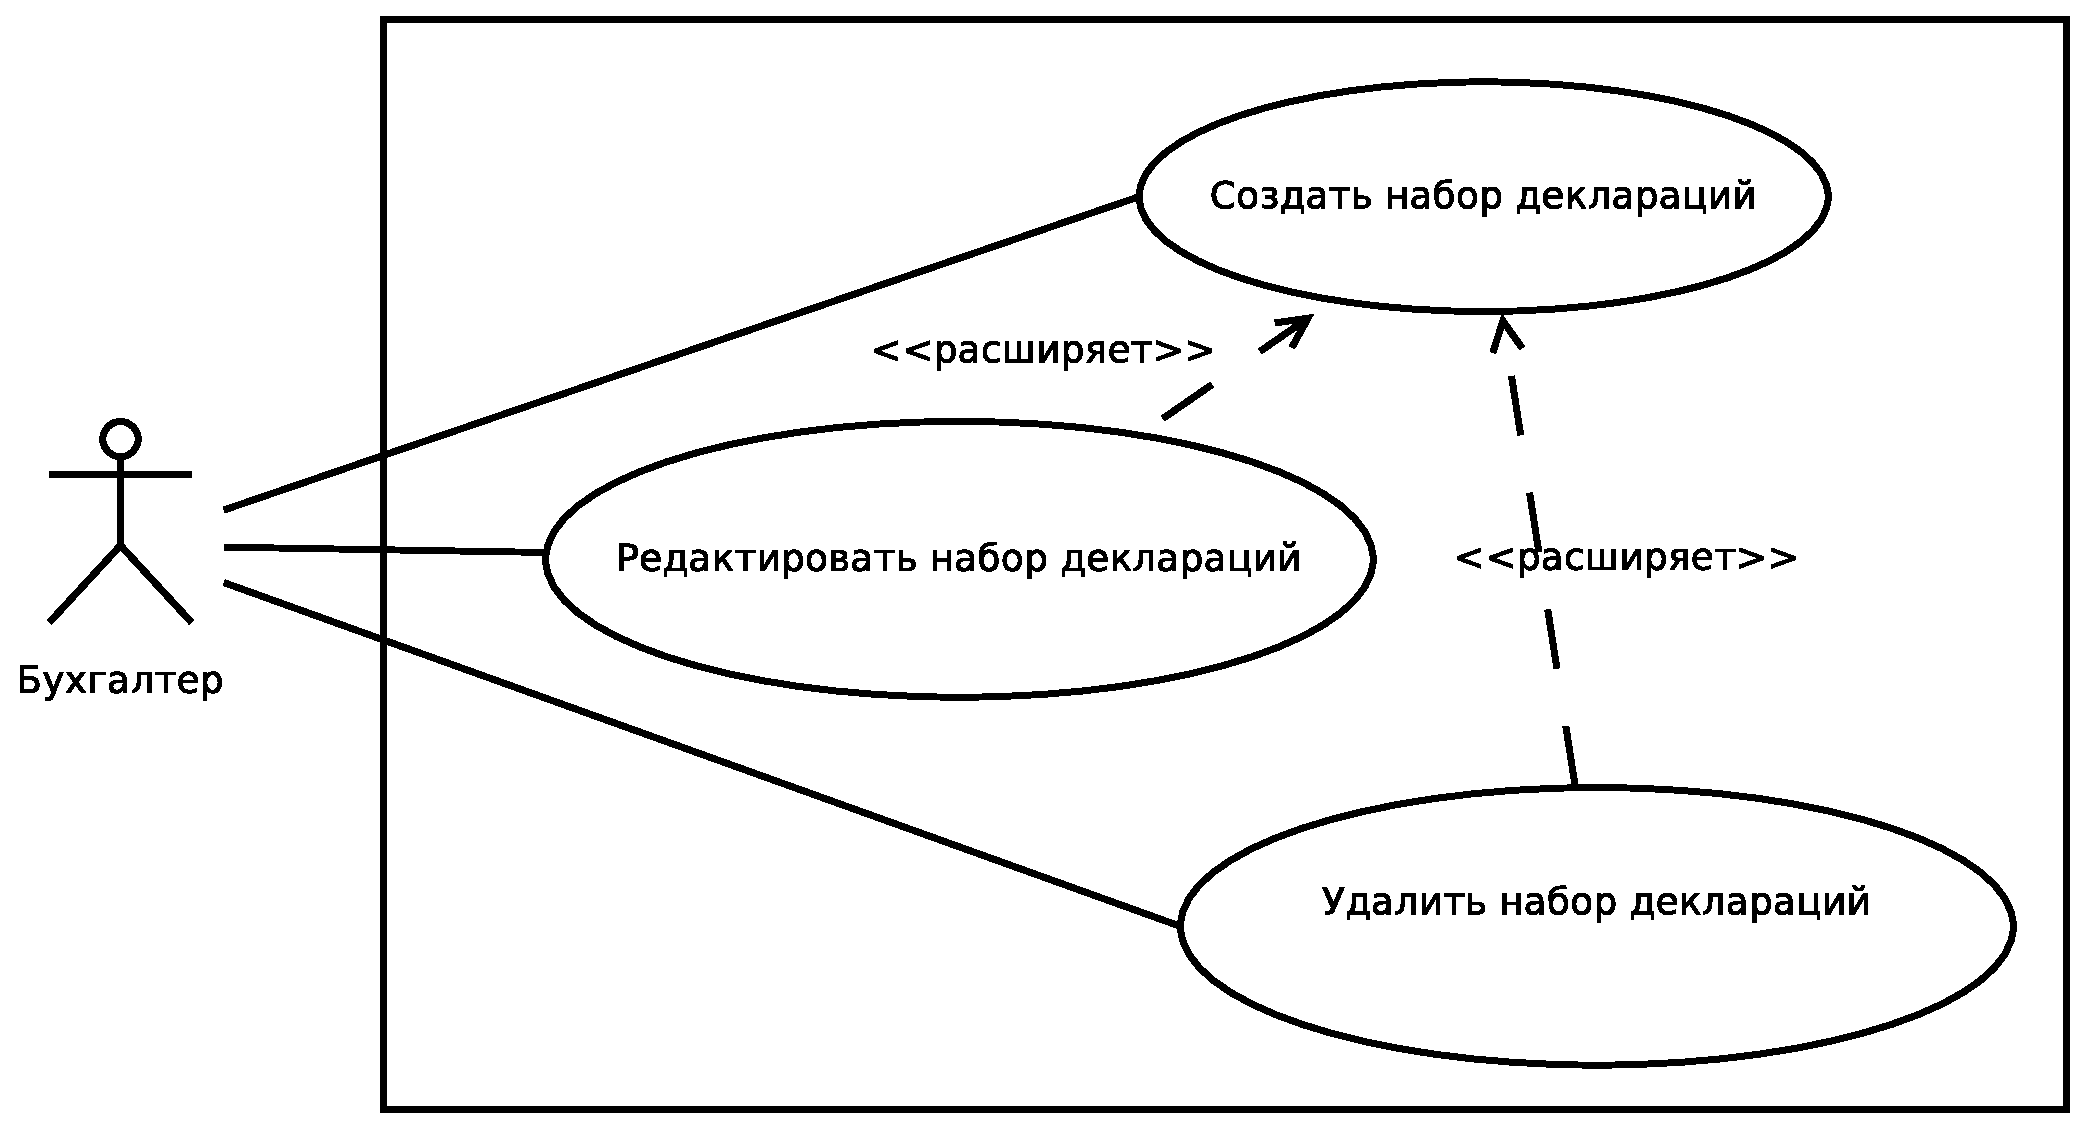
\includegraphics[scale=0.4]{uml/usecase_2}
  \caption{Диаграмма вариантов использования для работы с набором деклараций}
  \label{pic:use_case_2}
\end{figure}

\begin{sidewaysfigure}
  \centering
  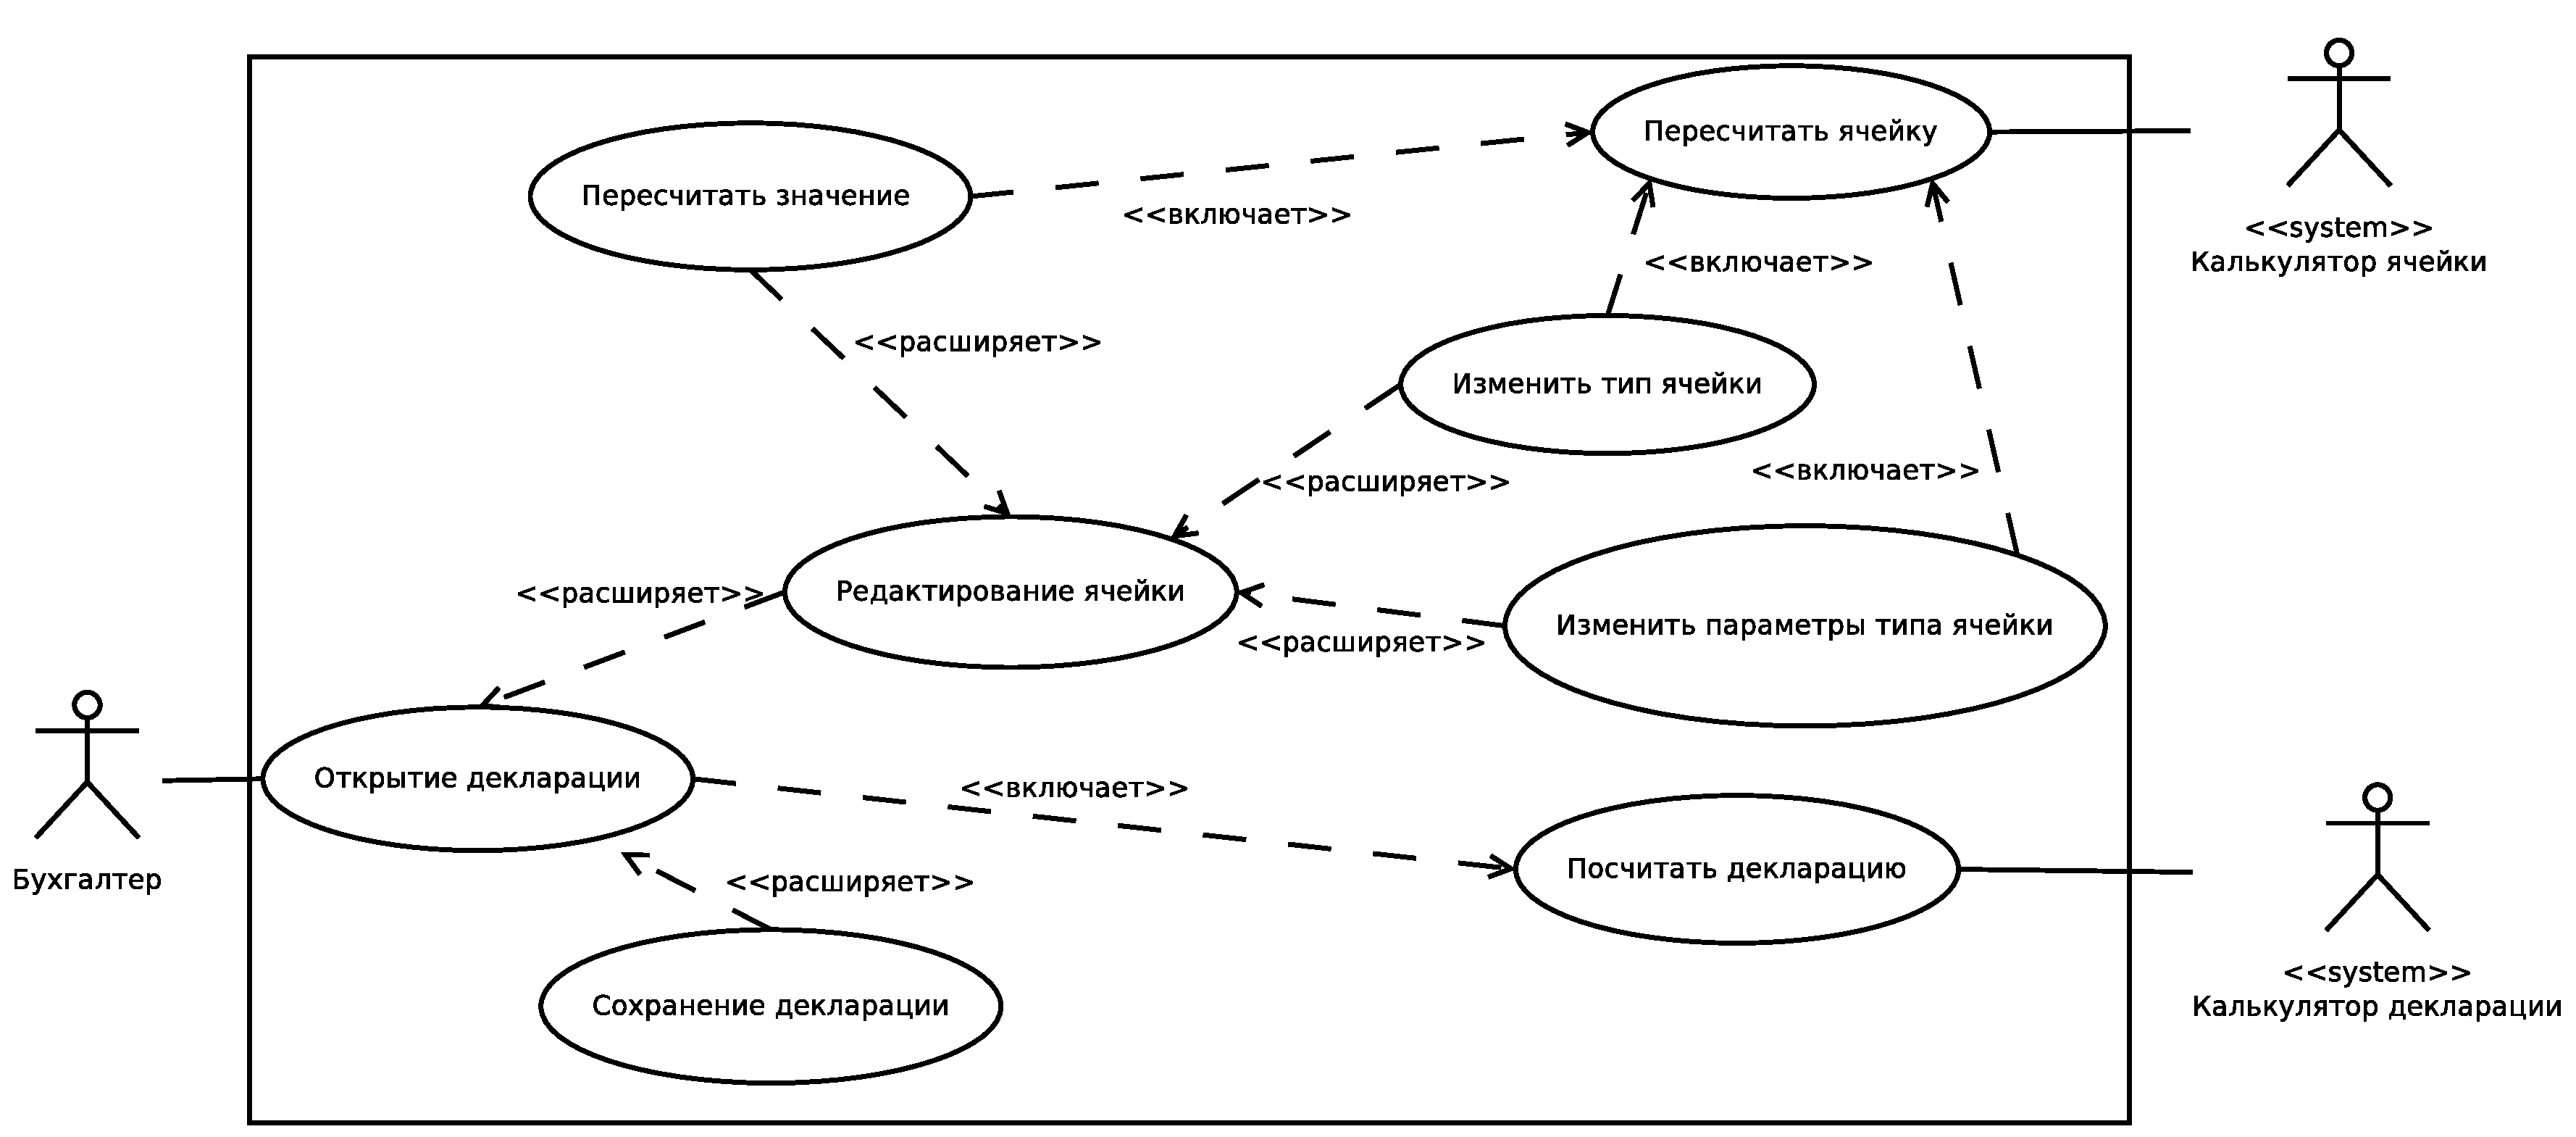
\includegraphics[scale=0.4]{uml/usecase_1}
  \caption{Диаграмма вариантов использования для работы с декларацией}
  \label{pic:use_case_1}
\end{sidewaysfigure}

Для отражения взаимодействия объектов системы приведем диаграммы последовательности.

Приведем диаграмму последовательности для вариантов использования при работе с компанией (рисунок~\ref{pic:sequence_1}).  Класс ``Сервис компании'' будет отвечать за работу с базой данных для объекта ``Компания''. При создании компании пользователь должен заполнить форму создания компании, затем ``Сервис компании'' сохранит созданную компанию. Для редактирования ``Сервис компании'' загружает сохраненную компанию, затем пользователь посредством формы редактирования изменяет параметры и ``Сервис компании'' сохраняет загруженный объект с новыми параметрами. Для удаления компании пользователь выбирает из списка существующих компаний компанию, которую он хочет удалить, ``Сервис компании'' удаляет выбранную пользователем компанию из базы данных.

\begin{figure}
  \centering
  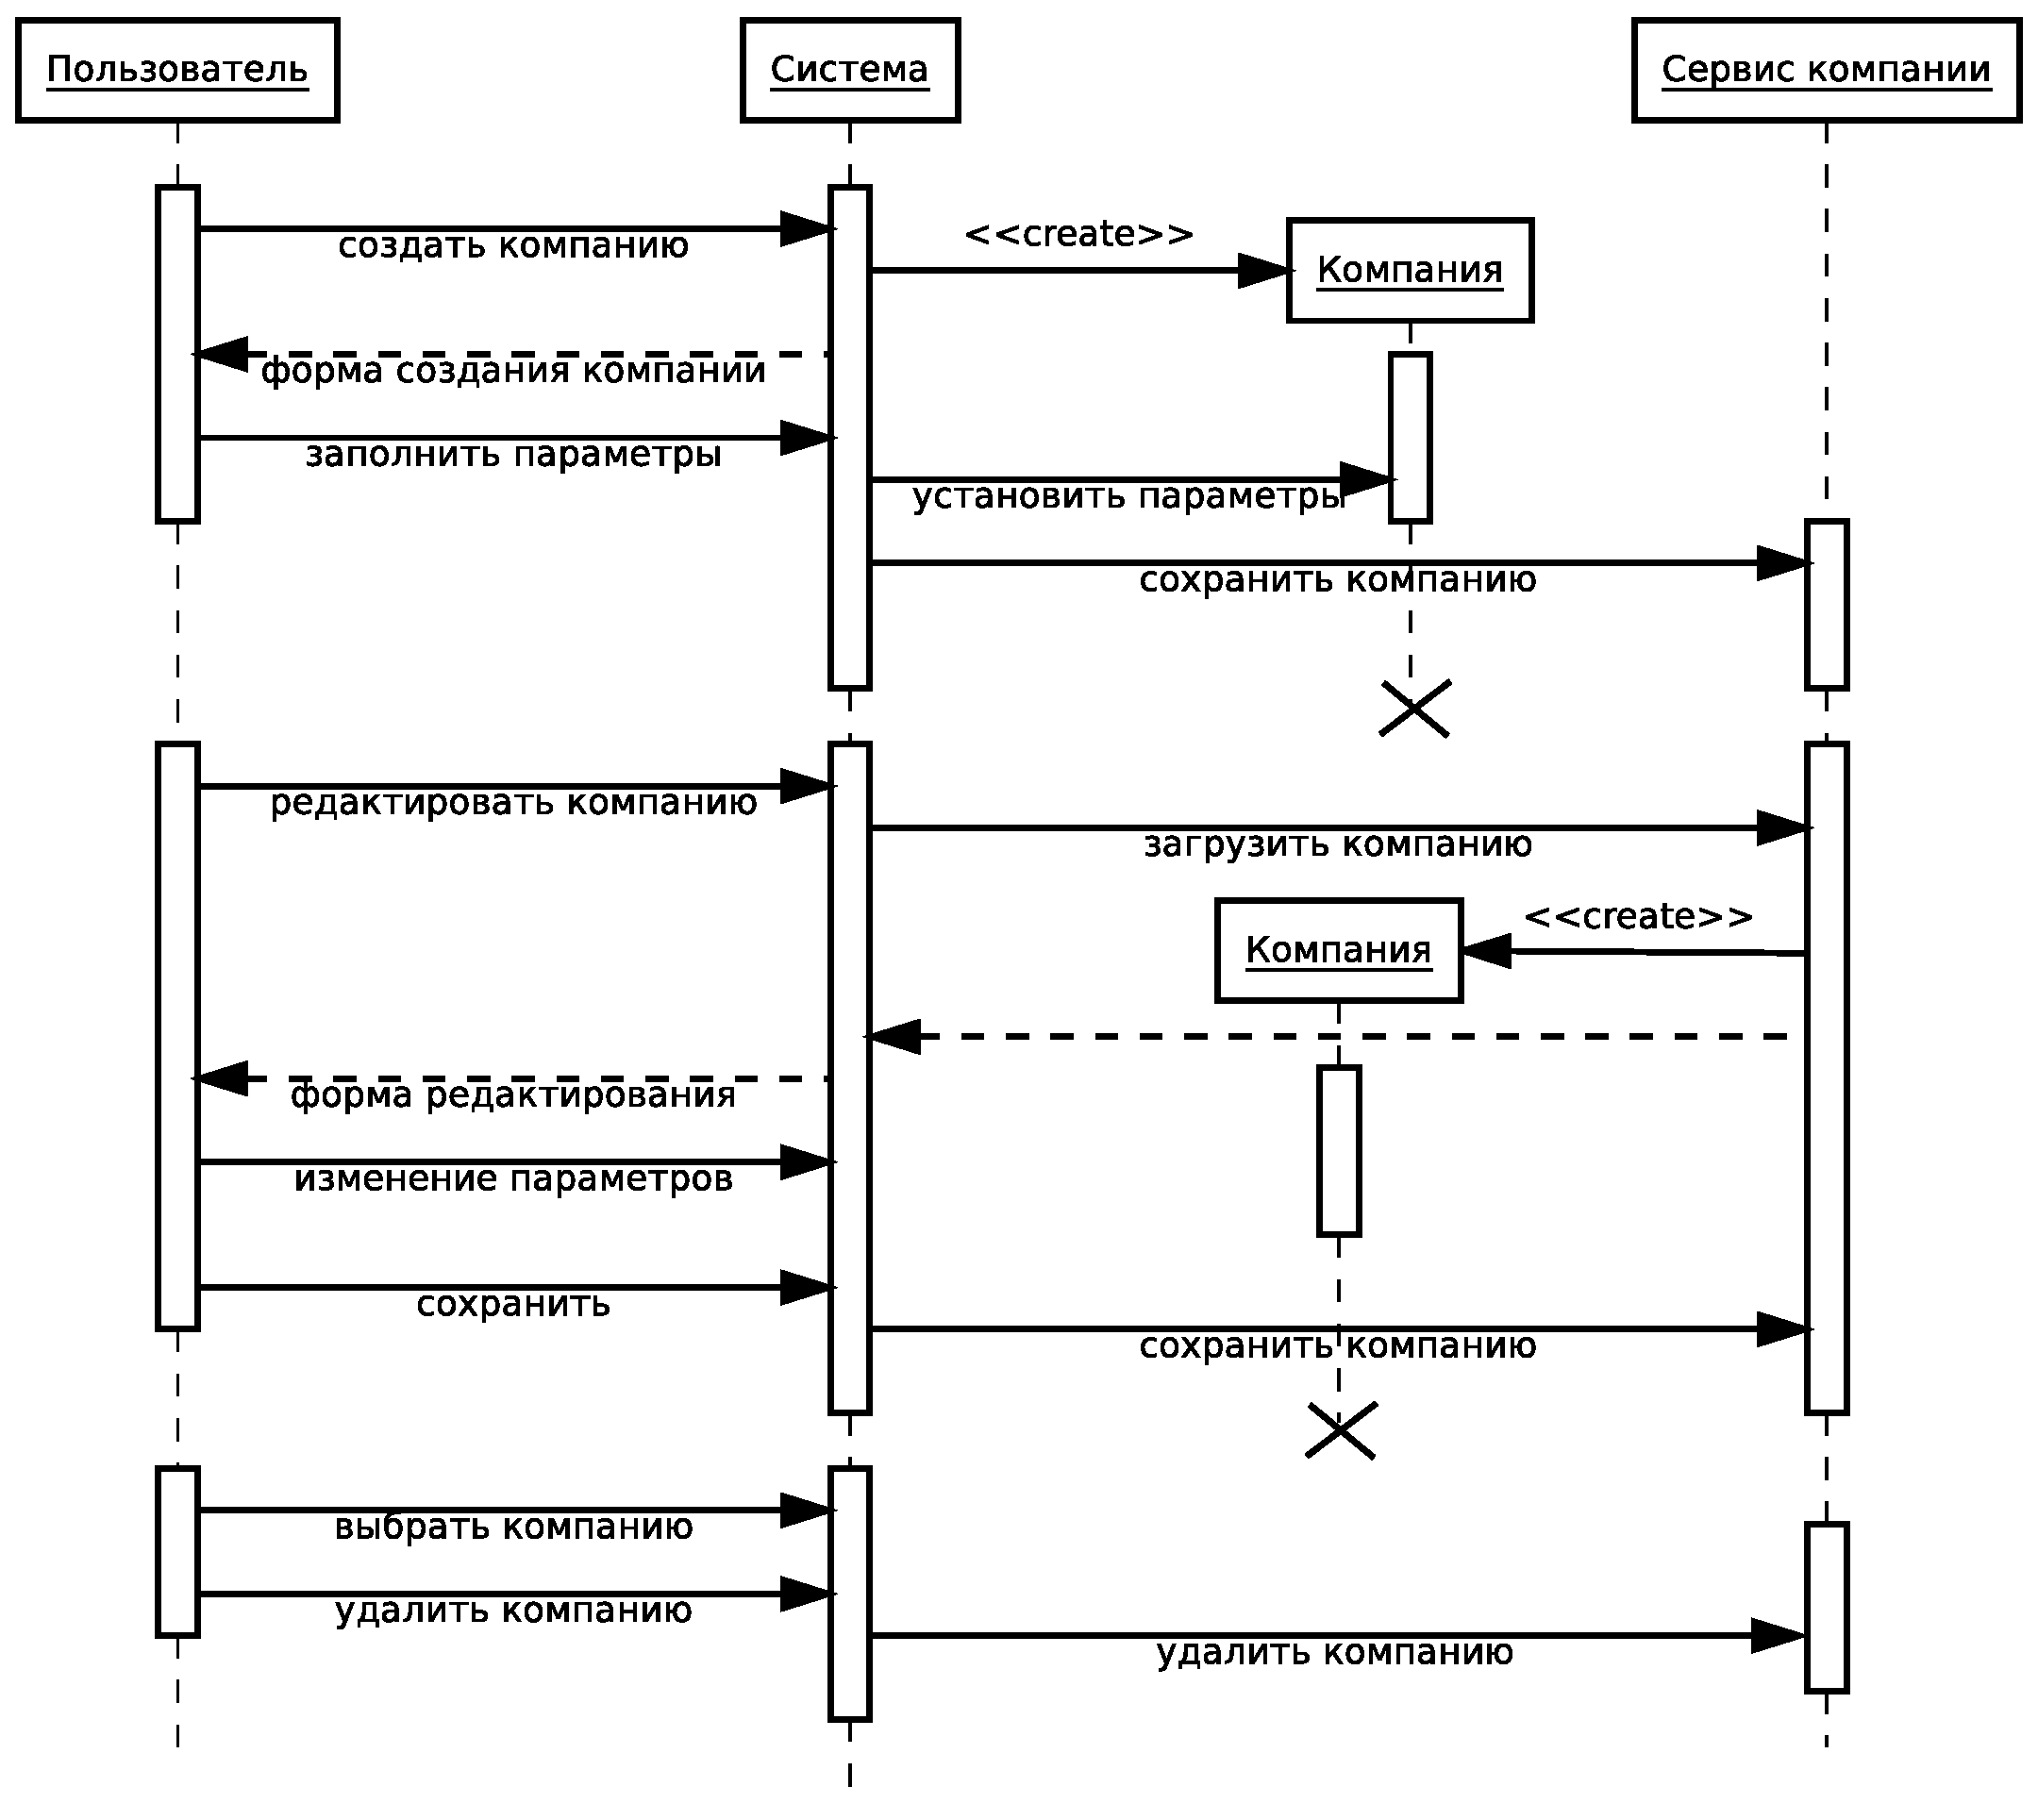
\includegraphics[scale=0.4]{uml/_sequence_4}
  \caption{Диаграмма последовательности для компании}
  \label{pic:sequence_1}
\end{figure}

Приведем диаграмму последовательности для работы с бухгалтерской книгой (рисунок~\ref{pic:sequence_2}). Пользователь создает бухгалтерскую книгу посредством формы создания, далее задает параметры для объекта, после чего значения параметров устанавливаются у созданного объекта ``Бухгалтерская книга''. При добавлении пользователем нового счета создается объект ``Счет'' и добавляется в ``Бухгалтерскую книгу''. При удалении счета на форме, счет удаляется из созданного объекта ``Бухгалтерская книга''. При изменении параметров счета на форме, параметры счета изменяются в созданном объекте ``Бухгалтерская книга''. За сохранение ``Бухгалтерской книги'' в базе данных отвечает класс ``Сервис Бухгалтерской книги''.

\begin{sidewaysfigure}
  \centering
  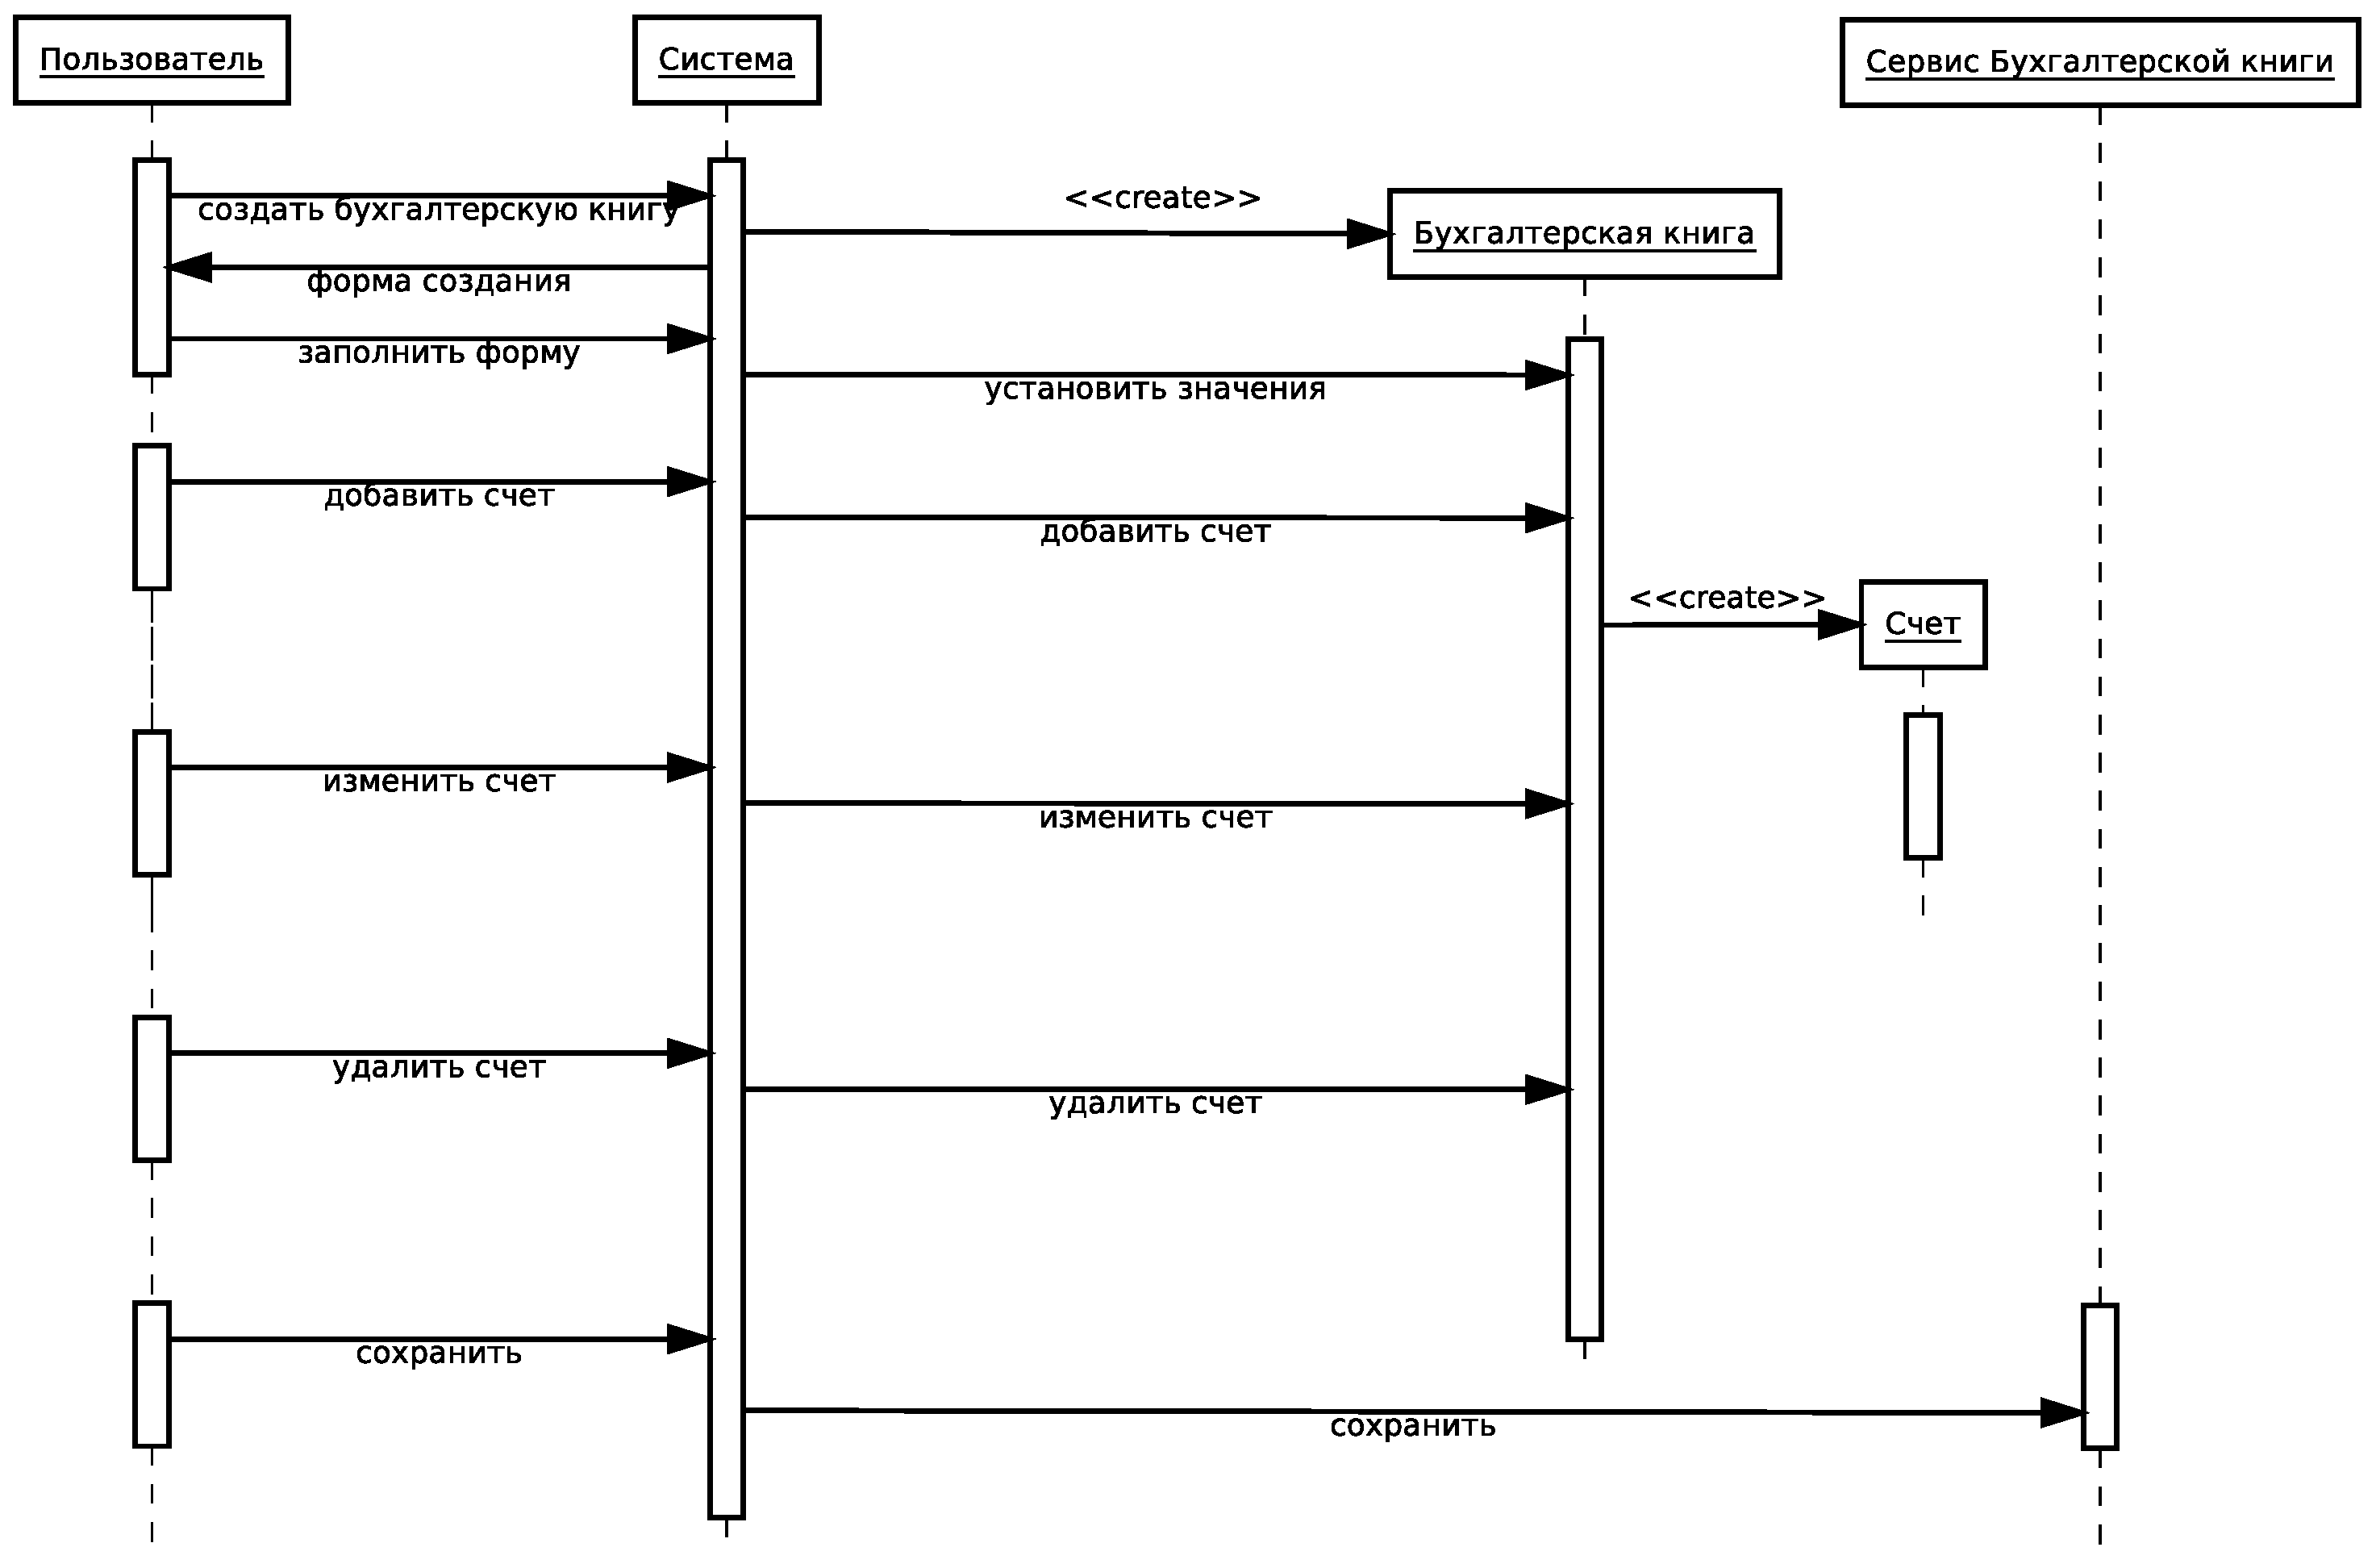
\includegraphics[scale=0.4]{uml/_sequence_5}
  \caption{Диаграмма последовательности для бухгалтерской книги}
  \label{pic:sequence_2}
\end{sidewaysfigure}

Приведем диаграмму последовательности для работы с налоговыми формами. Класс ``Сервис Налоговых форм'' будет отвечать за работу с базой данных для объекта ``Налоговые формы''. При создании налоговых форм пользователь должен заполнить форму необходимыми параметрами, во время создания пользователем налоговых форм создается объект ``Налоговые формы''. Посредством пользовательского интерфейса, пользователь задает параметры, после того как параметры заданы, объект ``Налоговые формы'' сохраняется в базе данных, за сохранение отвечает объект ``Сервис Налоговых форм''. Для редактирования налоговые формы загружаются из базы данных при помощи объекта ``Сервис Налоговых форм''. Далее, посредством интерфейса пользователя, пользователь изменяет параметры объекта, после чего объект ``Сервис Налоговых форм'' сохраняет измененный объект в базе данных. Для удаления, пользователю необходимо выбрать нужные налоговые формы, класс ``Сервис Налоговых форм'' удалит формы из базы данных.

\begin{figure}
  \centering
  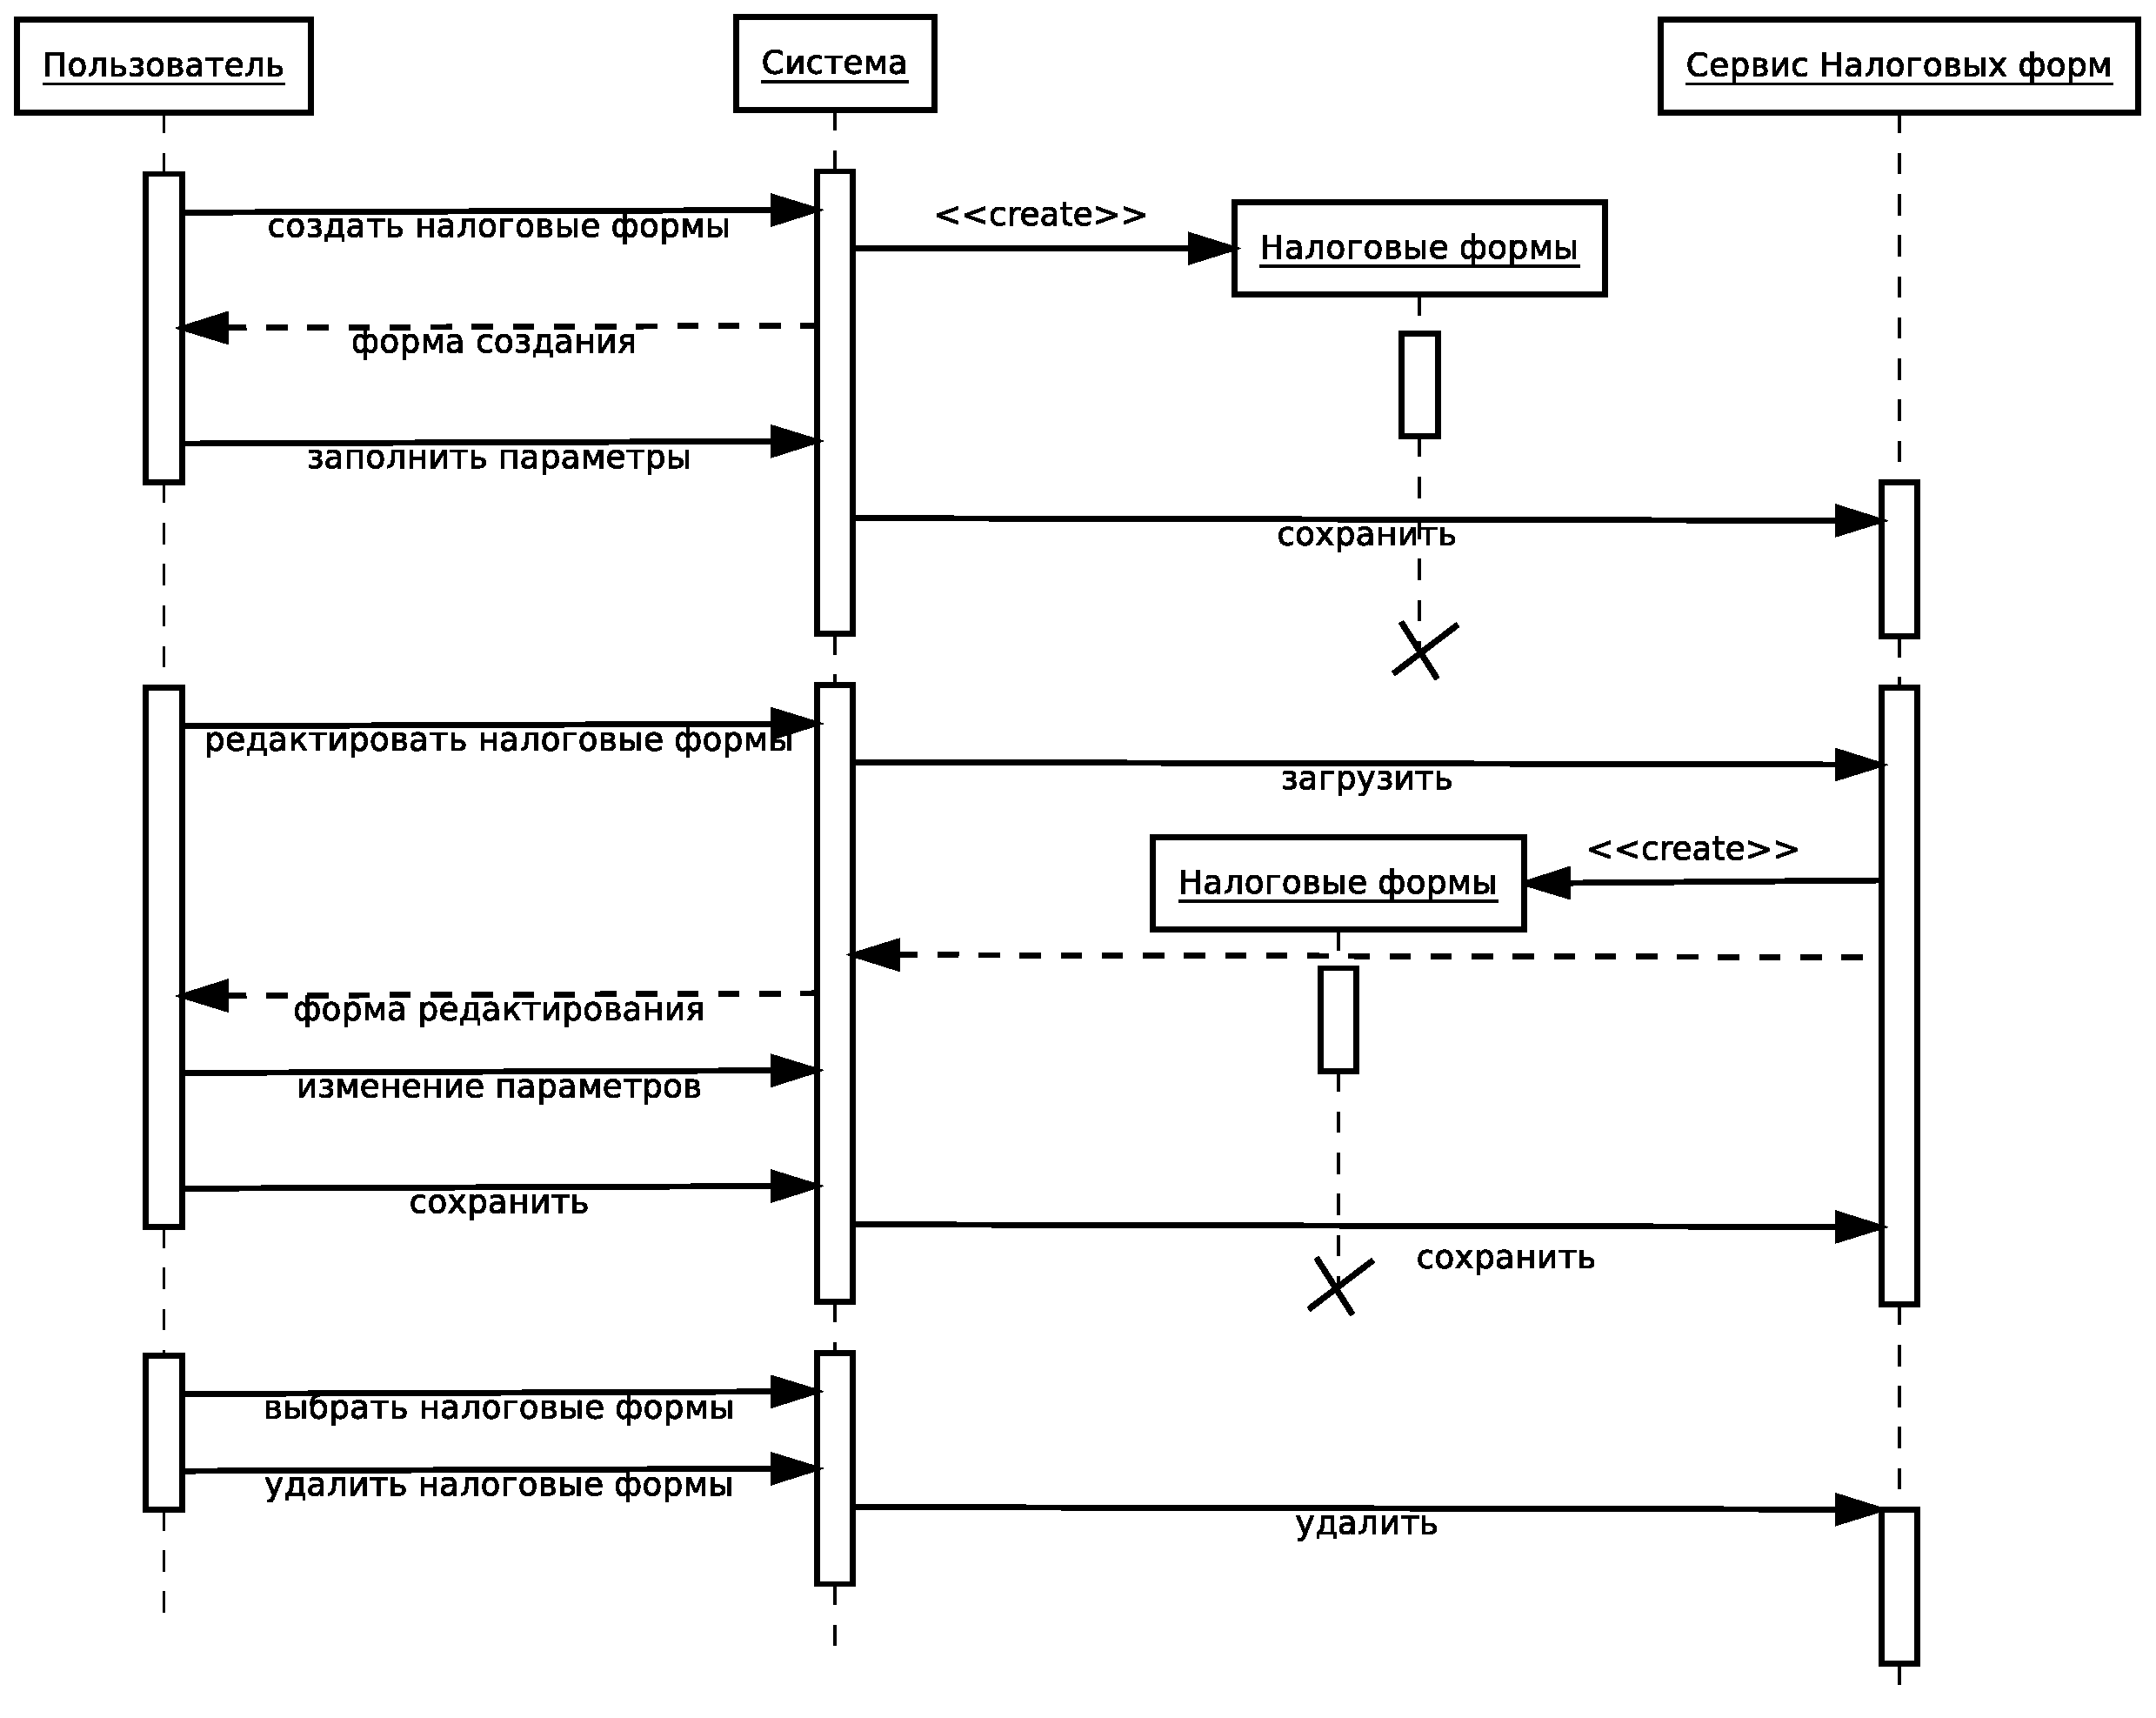
\includegraphics[scale=0.4]{uml/_sequence_6}
  \caption{Диаграмма последовательности для налоговых форм}
  \label{pic:sequence_3}
\end{figure}

Приведем диаграмму последовательности для открытия декларации (рисунок~\ref{pic:sequence_4}). Введем новый класс ``Сервис декларации'', который будет отвечать за работу с ``Декларацией'': загрузка структуры декларации (ячейки, типы ячеек, параметры типов ячеек ``по умолчанию'') и загрузку состояния декларации (значения ячеек, параметры типов ячеек). ``Сервис декларации'' при загрузке декларации создает объект ``Декларация'' и, если декларация уже была сохранена (открыта не первый раз), устанавливает сохраненное состояние. После загрузки декларации, ``Калькулятор декларации'' подсчитывает значение ячеек декларации (и устанавливает значения ячеек). Далее ``Пользовательский интерфейс'' отображает декларацию.

\begin{figure}
  \centering
  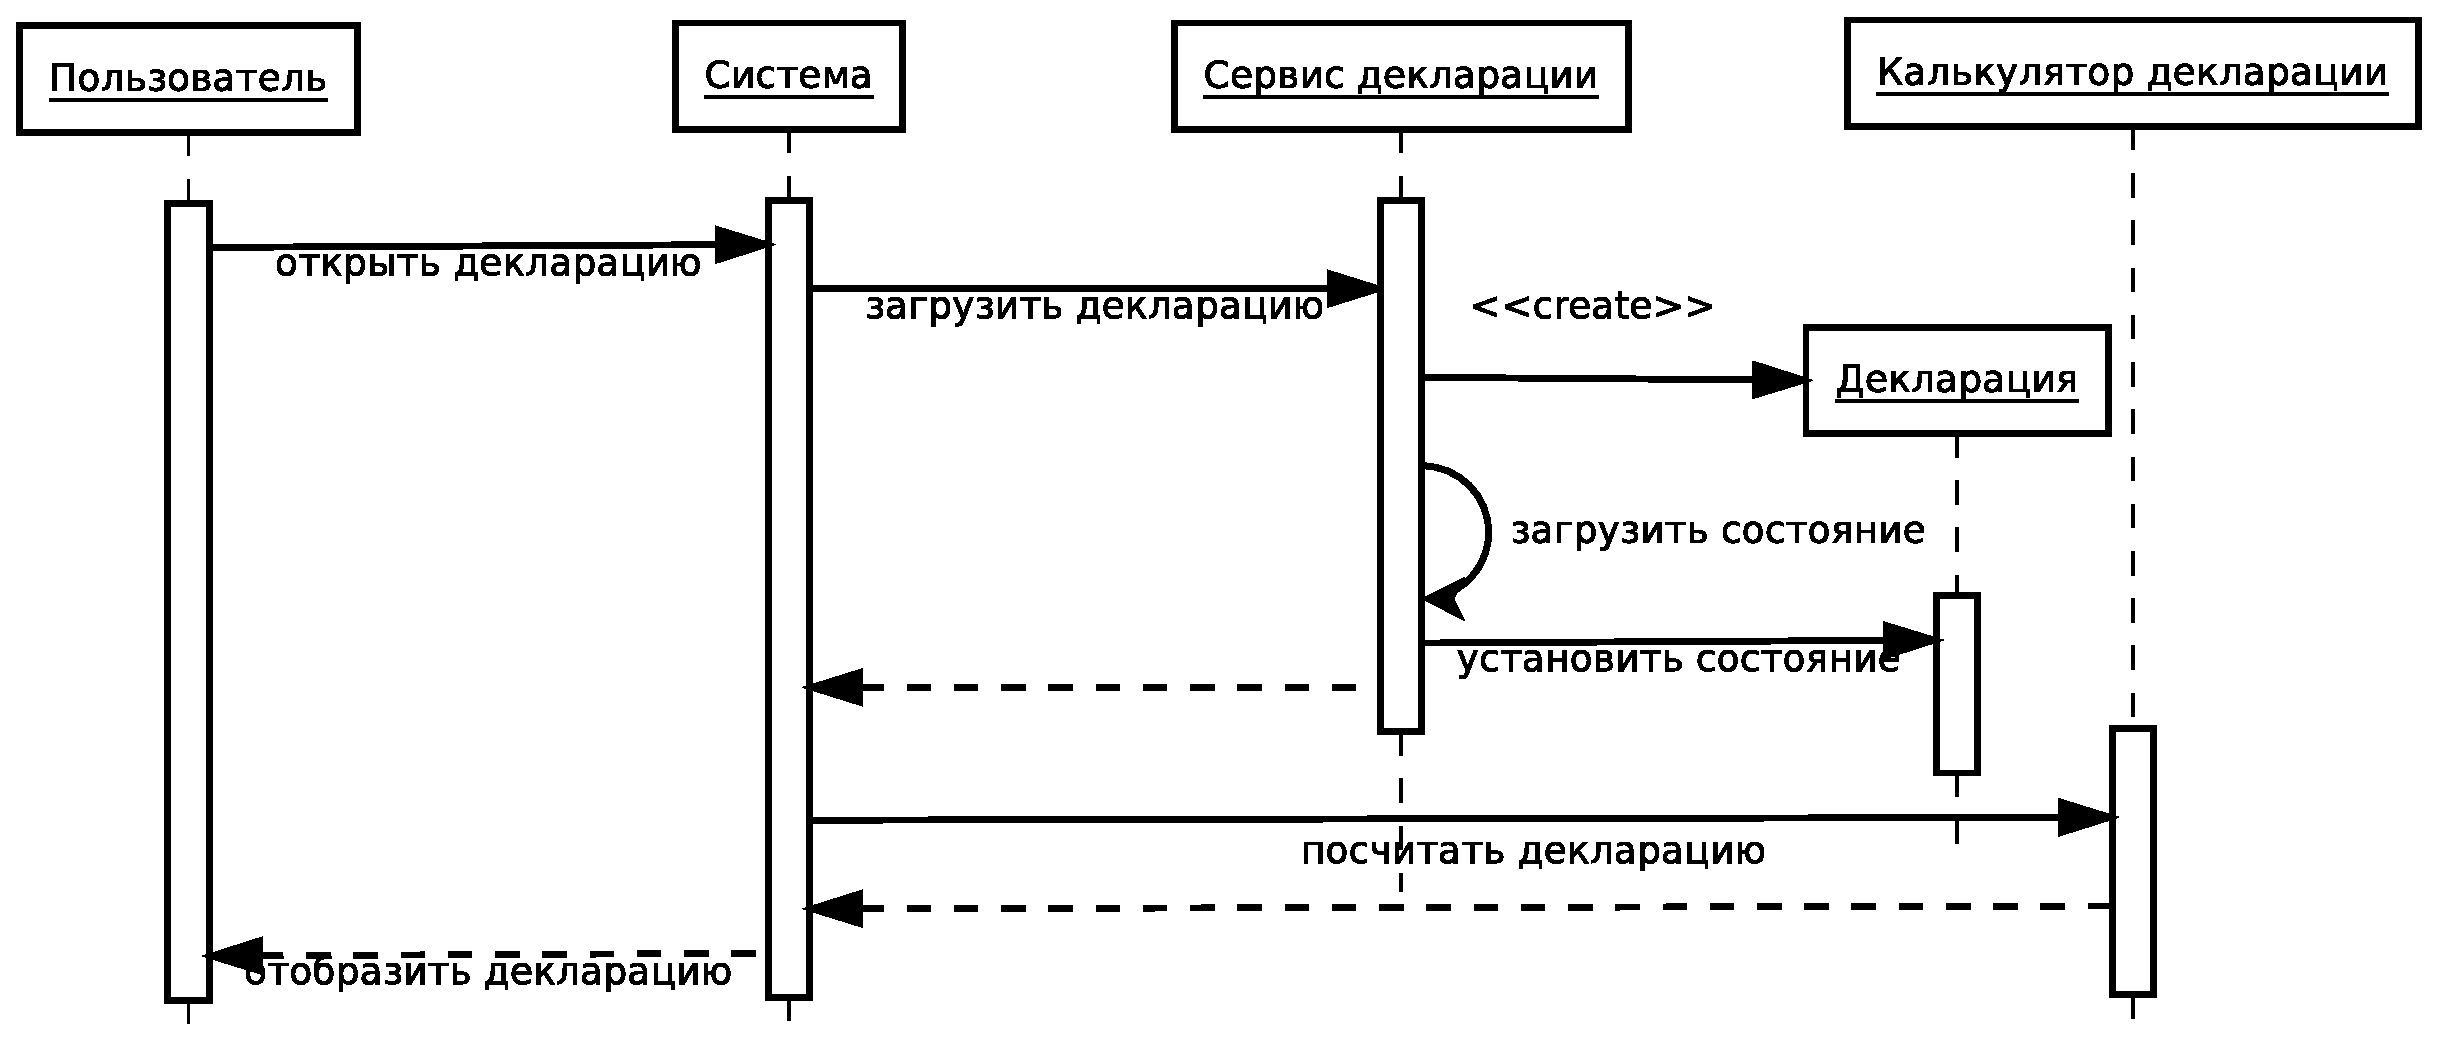
\includegraphics[scale=0.4]{uml/_sequence_1}
  \caption{Диаграмма последовательности для открытия декларации}
  \label{pic:sequence_4}
\end{figure}

На рисунке \ref{pic:sequence_4} изображена диаграмма последовательности для редактирования ячейки. Изменение типа ячейки происходит установкой типа ``Состояния ячейки''. После изменения типа ячейки необходим пересчет ячейки, который производится ``Калькулятором ячейки''. Изменение параметров типа ячейки происходит с помощью установки параметров объекта ``Состояние ячейки'', после установки новых параметров ячейка пересчитывается ``Калькулятором ячейки''.

\begin{sidewaysfigure}
  \centering
  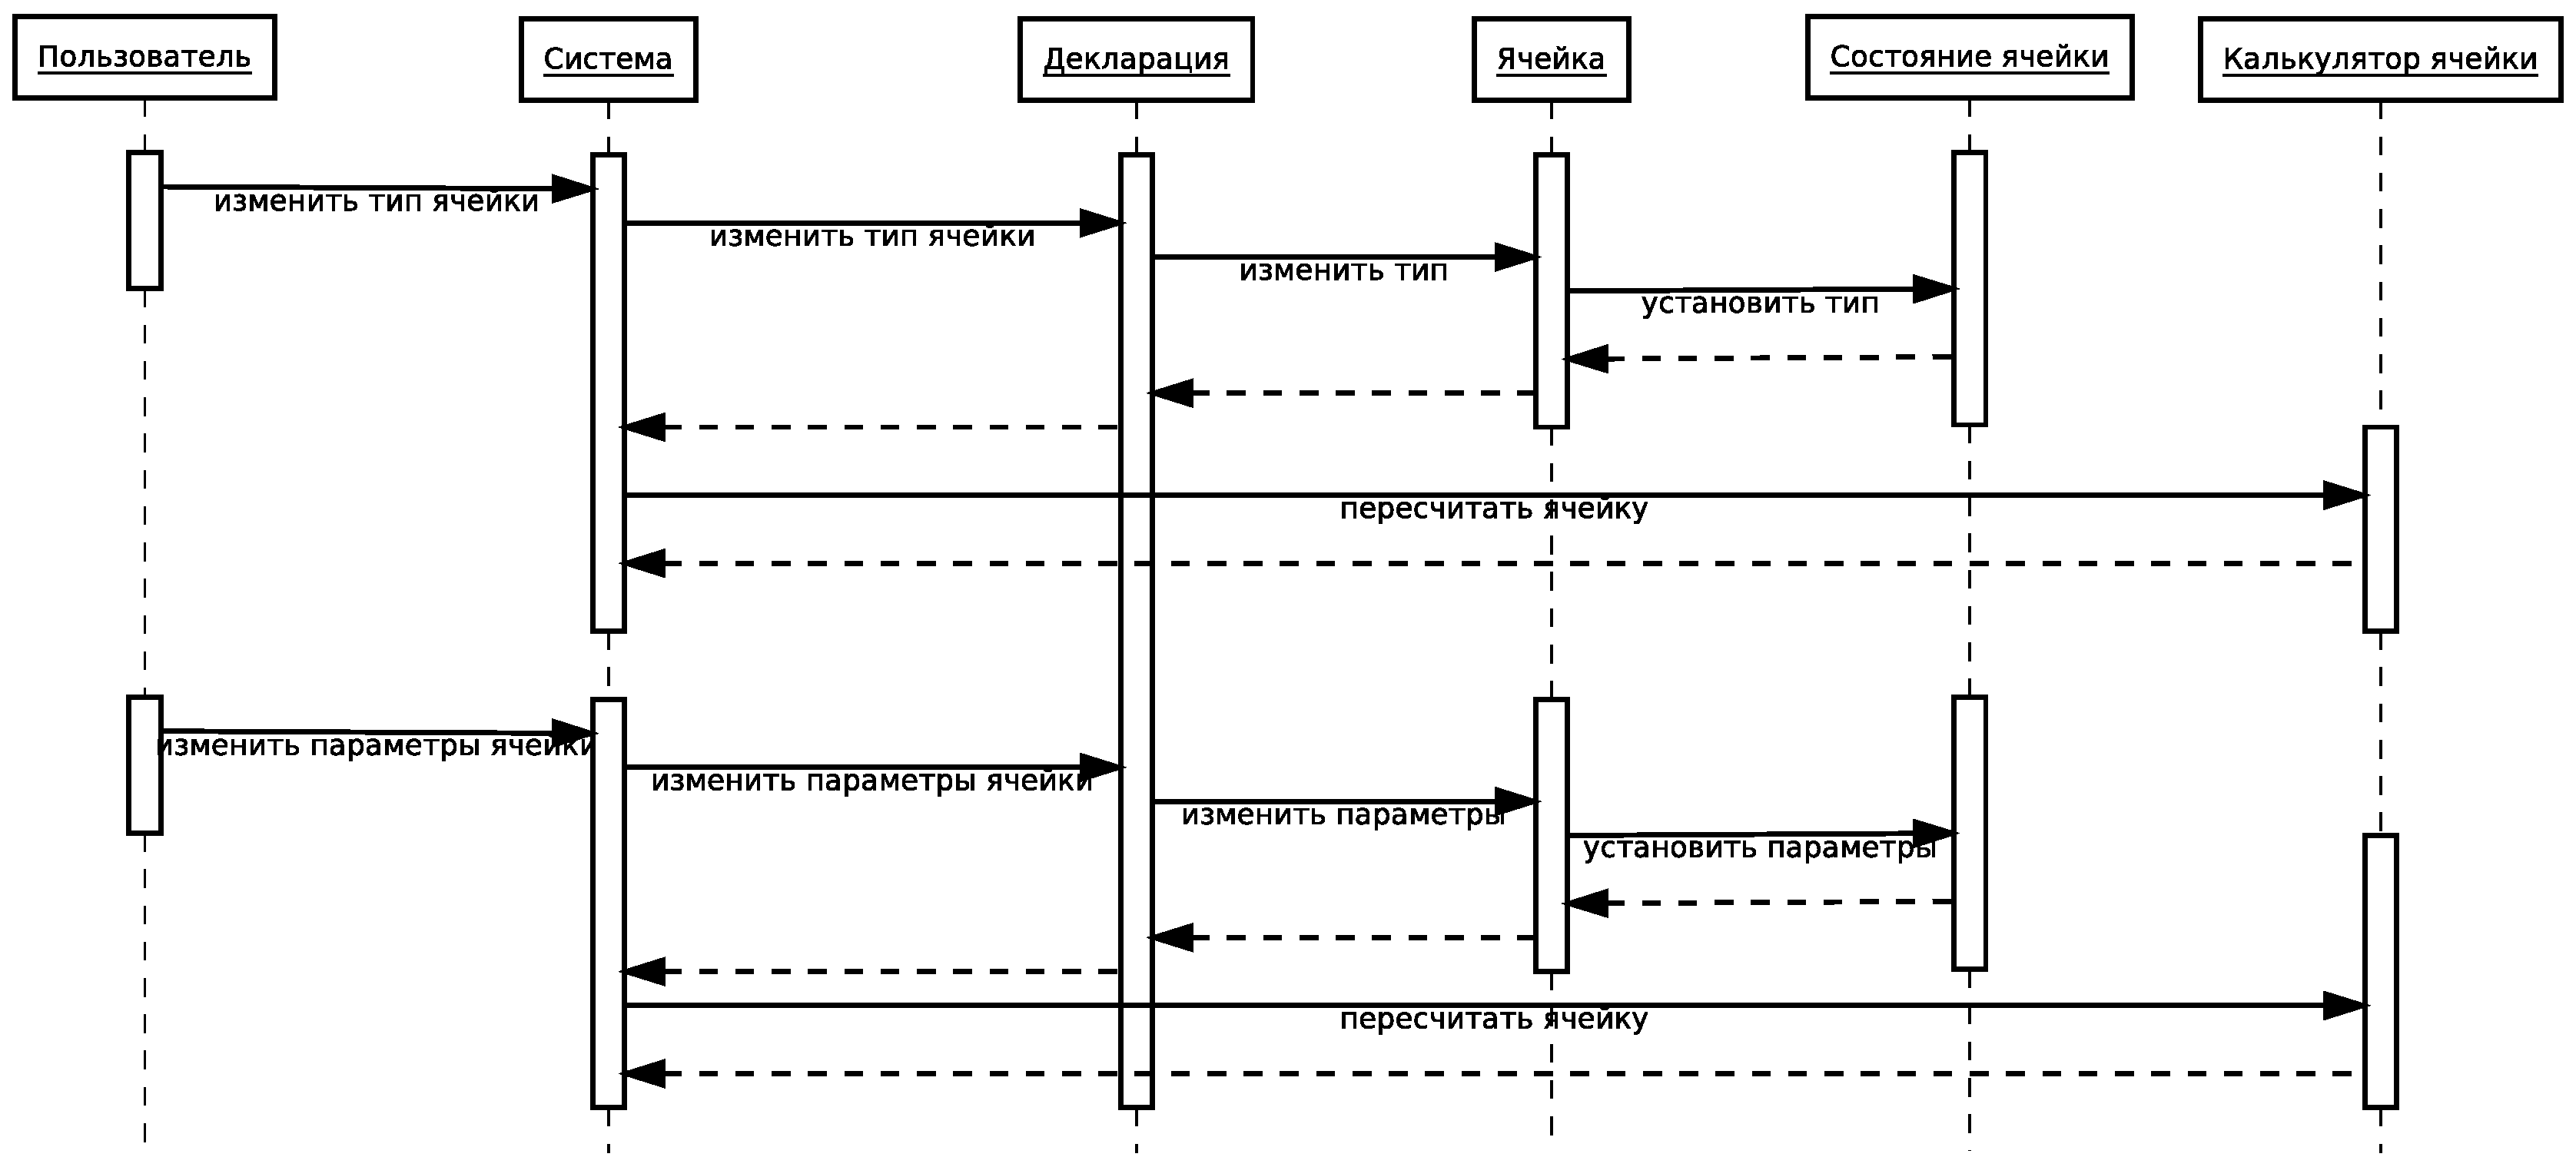
\includegraphics[scale=0.4]{uml/_sequence_2}
  \caption{Диаграмма последовательности для редактирования ячейки}
  \label{pic:sequence_4}
\end{sidewaysfigure}

Небольшая диаграмма последовательности для сохранения декларации приведена на рисунке \ref{pic:sequence_5}. Пользователь сообщает системе о том, что хочет сохранить декларацию, ``Сервис декларации'' сохраняет декларацию.

\begin{figure}
  \centering
  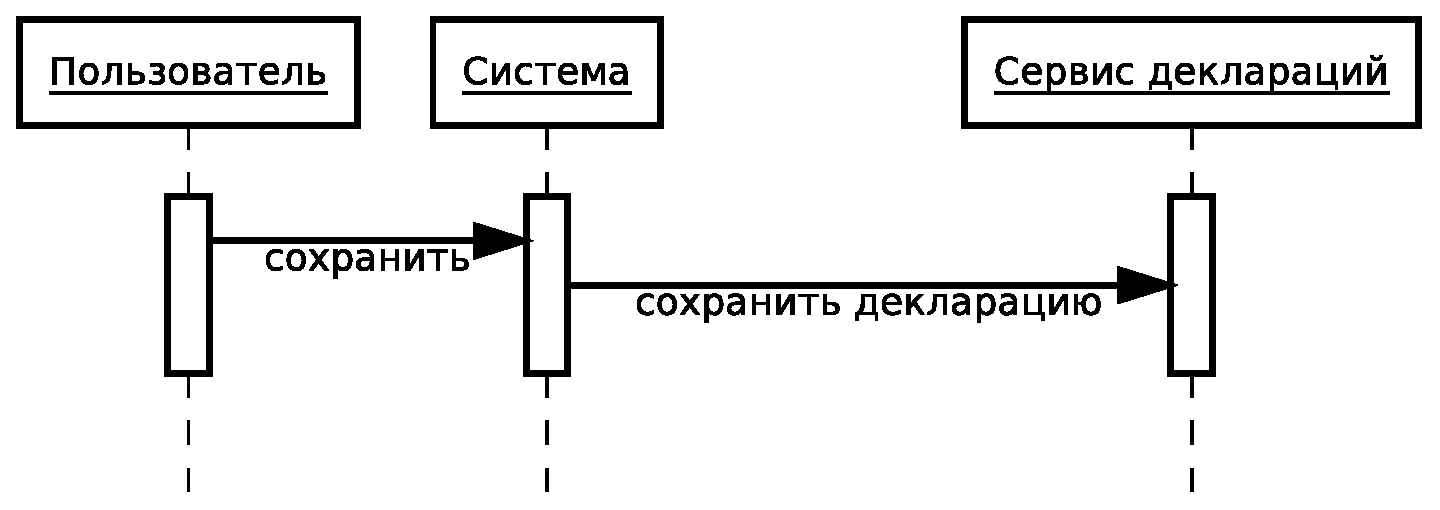
\includegraphics[scale=0.4]{uml/_sequence_3}
  \caption{Диаграмма последовательности для сохранения декларации}
  \label{pic:sequence_5}
\end{figure}

Для представления о динамике поведения объектов в системе приведем диаграммы состояний. Рассмотрим диаграмму состояний для открытия декларации (рисунок \ref{pic:states_1}). При открытии декларации загружается структура декларации, которая содержит свойства декларации ( в данный момент выделено ``название'' ), список ячеек с их параметрами. Далее, осуществляется попытка загрузки уже сохраненного состояния, если пользователь открывал данную декларацию и сохранил её, то загружается сохраненное состояние, иначе создается состояние, с параметрами, определенными по умолчанию. Затем производится установка загруженных состояний, либо состояний созданных с параметрами, которые заданы по умолчанию. После того как состояния установлены, производиться подсчет значений ячеек декларации.

\begin{figure}
  \centering
  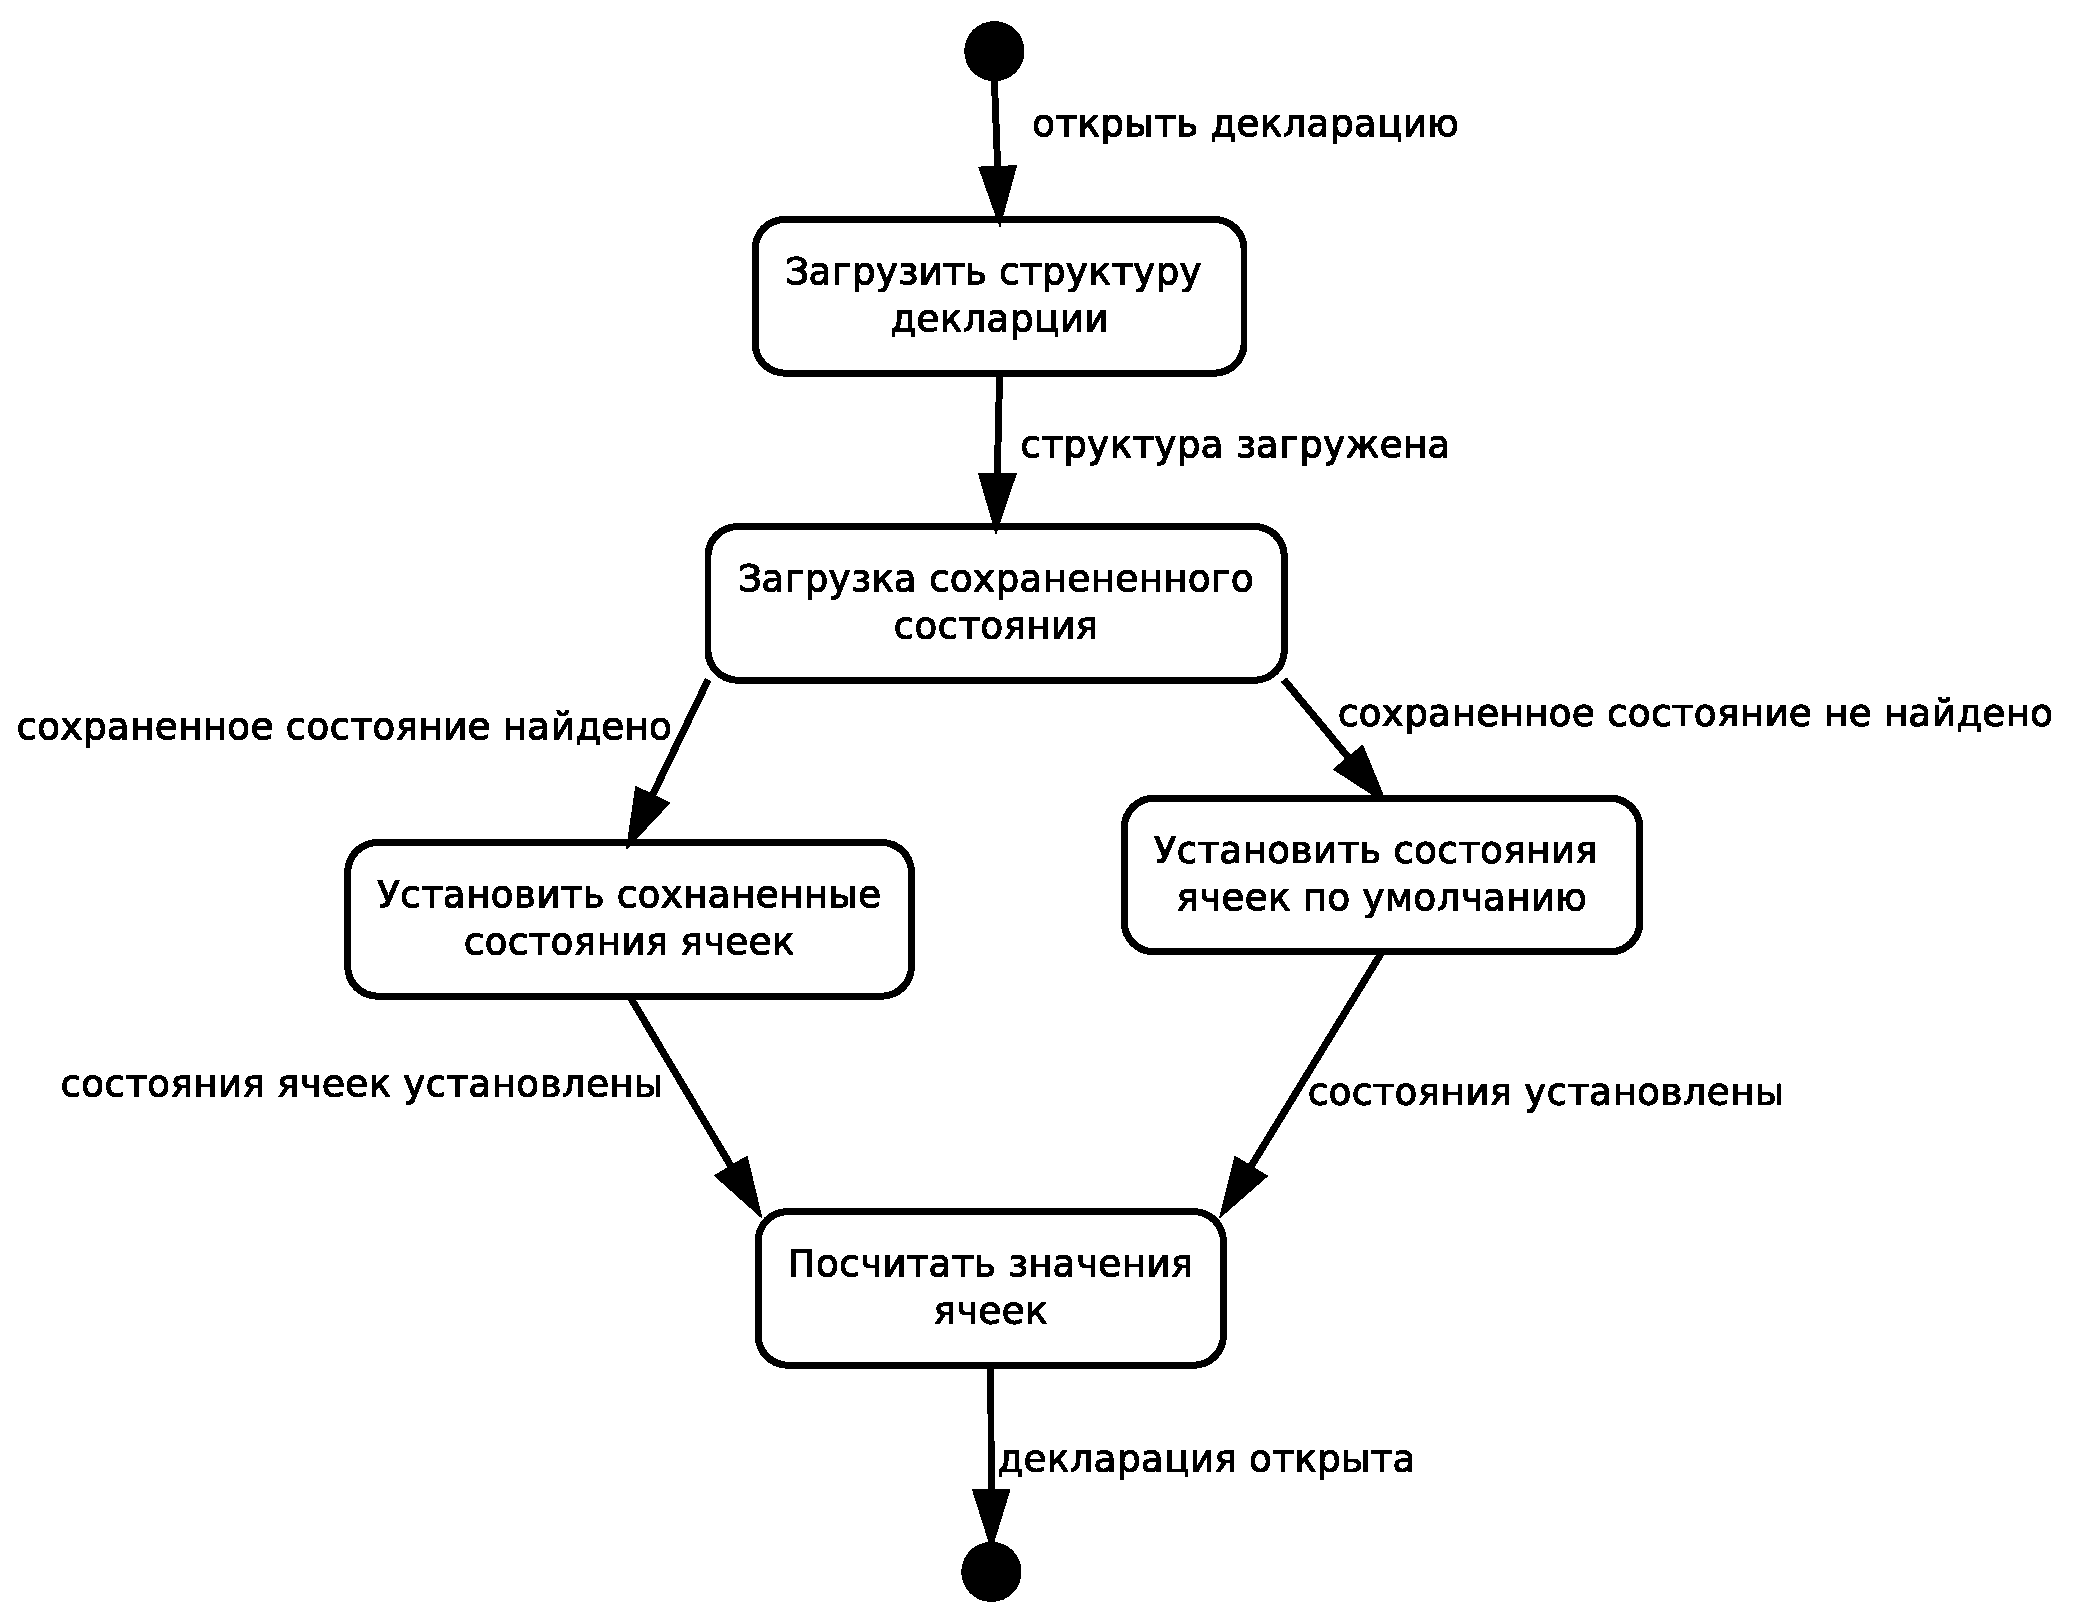
\includegraphics[scale=0.4]{uml/states_1}
  \caption{Диаграмма состояний для открытия деклараций}
  \label{pic:states_1}
\end{figure}

\subsection{Создания прототипа пользовательского интерфейса}

Процесс коммуникации системы с пользователем будет осуществляться посредством графического пользовательского интерфейса. На основании вариантов использования создадим прототип пользовательского интерфейса, рассмотрим каждый вариант использования.

На диаграмме вариантов использования для работы с компанией пользователю необходимо осуществлять создание, редактирования и удаление сущности ``Компания''. Создание и редактирование объекта может осуществляться посредством формы, на которой содержатся элементы ввода для параметров ``Компании''.
%todo:привести пример формы
Для удаления и редактирования компании, пользователю необходимо осуществить выбор компании, которую он хотел бы редактировать или изменить. Для этих целей можно предоставить пользователю список, на котором будут изображены все созданные компании, с элементами управления, по нажатию на которые будет отображена форма редактирования, либо объект будет удален.
%todo:привести пример списка

Рассмотрим варианты использования для работы с бухгалтерской книгой. Для создания и редактирования ``Бухгалтерской книги'' необходимо предоставить пользователю форму, на которой будут располагаться элементы ввода для параметров бухгалтерской книги( ``Компания'' которой она будет принадлежать, ``название''). Для возможности добавления и редактирования ``Счетов'' бухгалтерской книги необходимо предоставить элементы, по нажатию на которые будет осуществлено добавление либо удаление ``Счета''. Для работы со ``Счетом'' необходимо предоставить панель, которая будет содержать элементы ввода для параметров ``Счета'' (``номер'', ``кредит'', ``дебет''). При добавлении счета на форме будет добавляться панель, при удалении счета, соответствующая ему панель будет удаляться.
%todo:привести пример формы бухгалтерской книги
Для возможности выбора пользователем бухгалтерской книги, которую он хотел бы удалить или отредактировать, необходимо использовать список, на котором будут отображаться созданные бухгалтерские книги.
%todo:привести пример списка бухгалтерской книги

Рассмотрим варианты использования для работы с налоговыми формами. Создания и редактирование ``Налоговыми формами'' будет осуществляться посредством формы на которой будут содержаться элементы выбора и ввода параметров объекта. Нужно учесть тот факт, что пользователю нужно выбрать ``Компанию'', затем для выбранной компании выбрать ``Бухгалтерскую книгу''.
%todo:привести пример формы создания редактирования налоговых форм
Для возможности выбора пользователем налоговых форм, которые он хотел бы отредактировать либо удалить, необходимо использовать список, на котором будут отображаться созданные налоговые формы, напротив каждой налоговой формы следует расположить элементы, по нажатию на которые будет отображена форма редактирования, либо удалена соответствующая налоговая форма. Так же для того что бы работать с декларациями, в списке напротив каждого объекта расположим элемент, состояние которого будет показывать выбран ли он в качестве активного. Пользователь будет работать именно с декларациями активных налоговых форм.
%todo:привести пример списка налоговых форм

Далее рассмотрим варианты использования для работы с декларацией. Для выбора декларации, которую необходимо открыть пользователю будет использоваться список доступных деклараций. Форма декларации должна содержать ячейки, которые будут представлять собой элементы ввода, в зависимости от типа ячейки они будут доступны, либо не доступны для редактирования (пользовательский тип ячейки будет доступна для редактирования, так как значение должен ввести пользователь). При выборе пользователем конкретной ячейки необходимо отобразить панель, которая будет содержать текущие параметры ячейки, в зависимости от типа ячейки будут содержаться элементы ввода для изменения параметров.
%todo:привести пример списка деклараций.
%todo:привести пример декларации.

\section{Детализация объектов}
Рассмотрим объекты системы на более низком уровне абстракции.

На рисунке~\ref{pic:classes_1} изобразим основные объекты системы. Был введен новый объект ``СостояниеДекларации'', являющийся представлением экземпляра декларации для ``НалоговыхФорм''. Данный объект имеет атрибут ``состоянияЯчеек'', который представляет собой список состояний всех ячеек декларации. Объект ``СостояниеЯчейки'' содержит атрибут ``типыЯчеек'', который представляет собой список ``ТиповЯчейки'', список содержит возможные типы, которые может представлять ячейка. Объект ``Значение'' содержит значение ячейки, объект был введен так как типы данных значений ячеек могут быть разными.

\begin{sidewaysfigure}
  \centering
  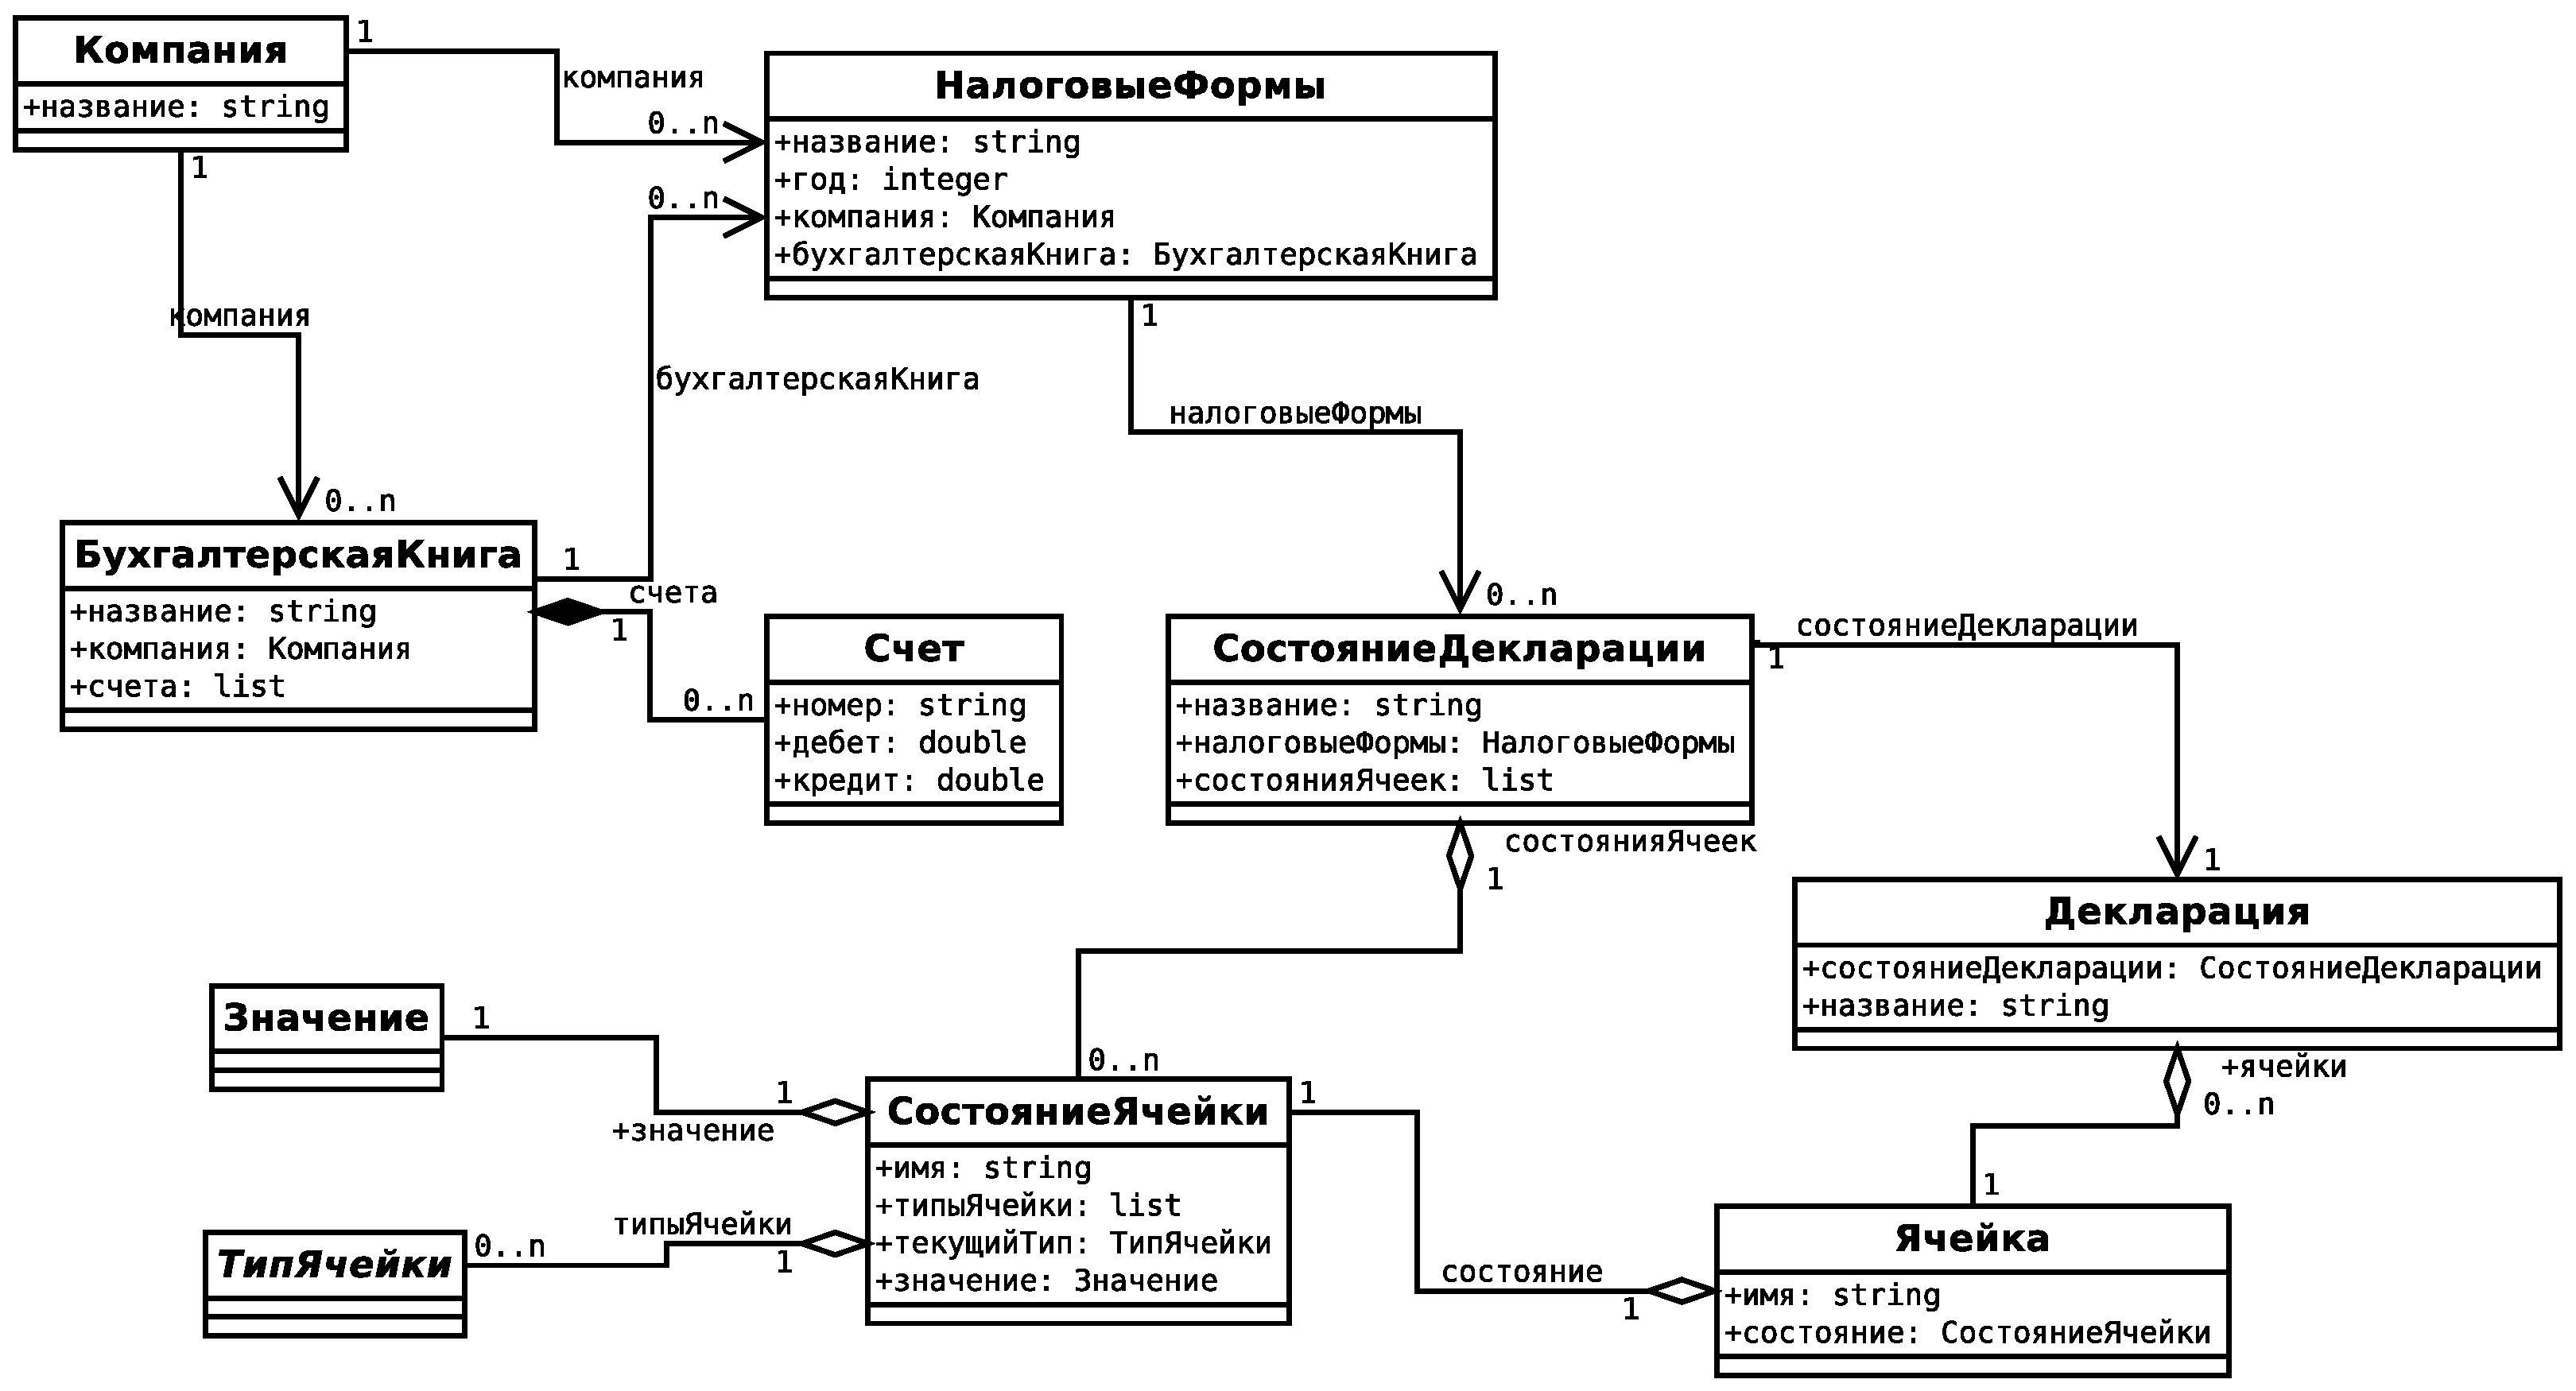
\includegraphics[scale=0.4]{uml/_classes_1}
  \caption{Диаграмма основных объектов системы}
  \label{pic:classes_1}
\end{sidewaysfigure}

Рассмотрим диаграмму, на которой приведены объекты, участвующие в подсчете декларации. ``КалькуляторДекларации'' содержит метод ``посчитатьДекларацию'', который подсчитывает значения ячеек декларации и устанавливает значения для ячеек. Метод ``пересчитатьЯчейку'' пересчитывает одну ячейку и возвращает список пересчитанных ячеек (включая данную), которые являются зависимыми от данной (например, если значение какой-либо формулы зависит от значения пересчитываемой ячейки, то при пересчете должна пересчитаться и формула). Объект ``Контекст''  содержит значения уже посчитанных ячеек, значение можно установить вызовом метода ``установитьЗначение'', для получения значения используется метод ``получитьЗначение''. Для подсчета значения каждой ячейки используется объект ``КалькуляторЯчейки'', данный объект содержит абстрактный метод ``посчитать'', который принимает в качестве параметров ``ТипЯчеки'' и ``Контекст''.

\begin{figure}
  \centering
  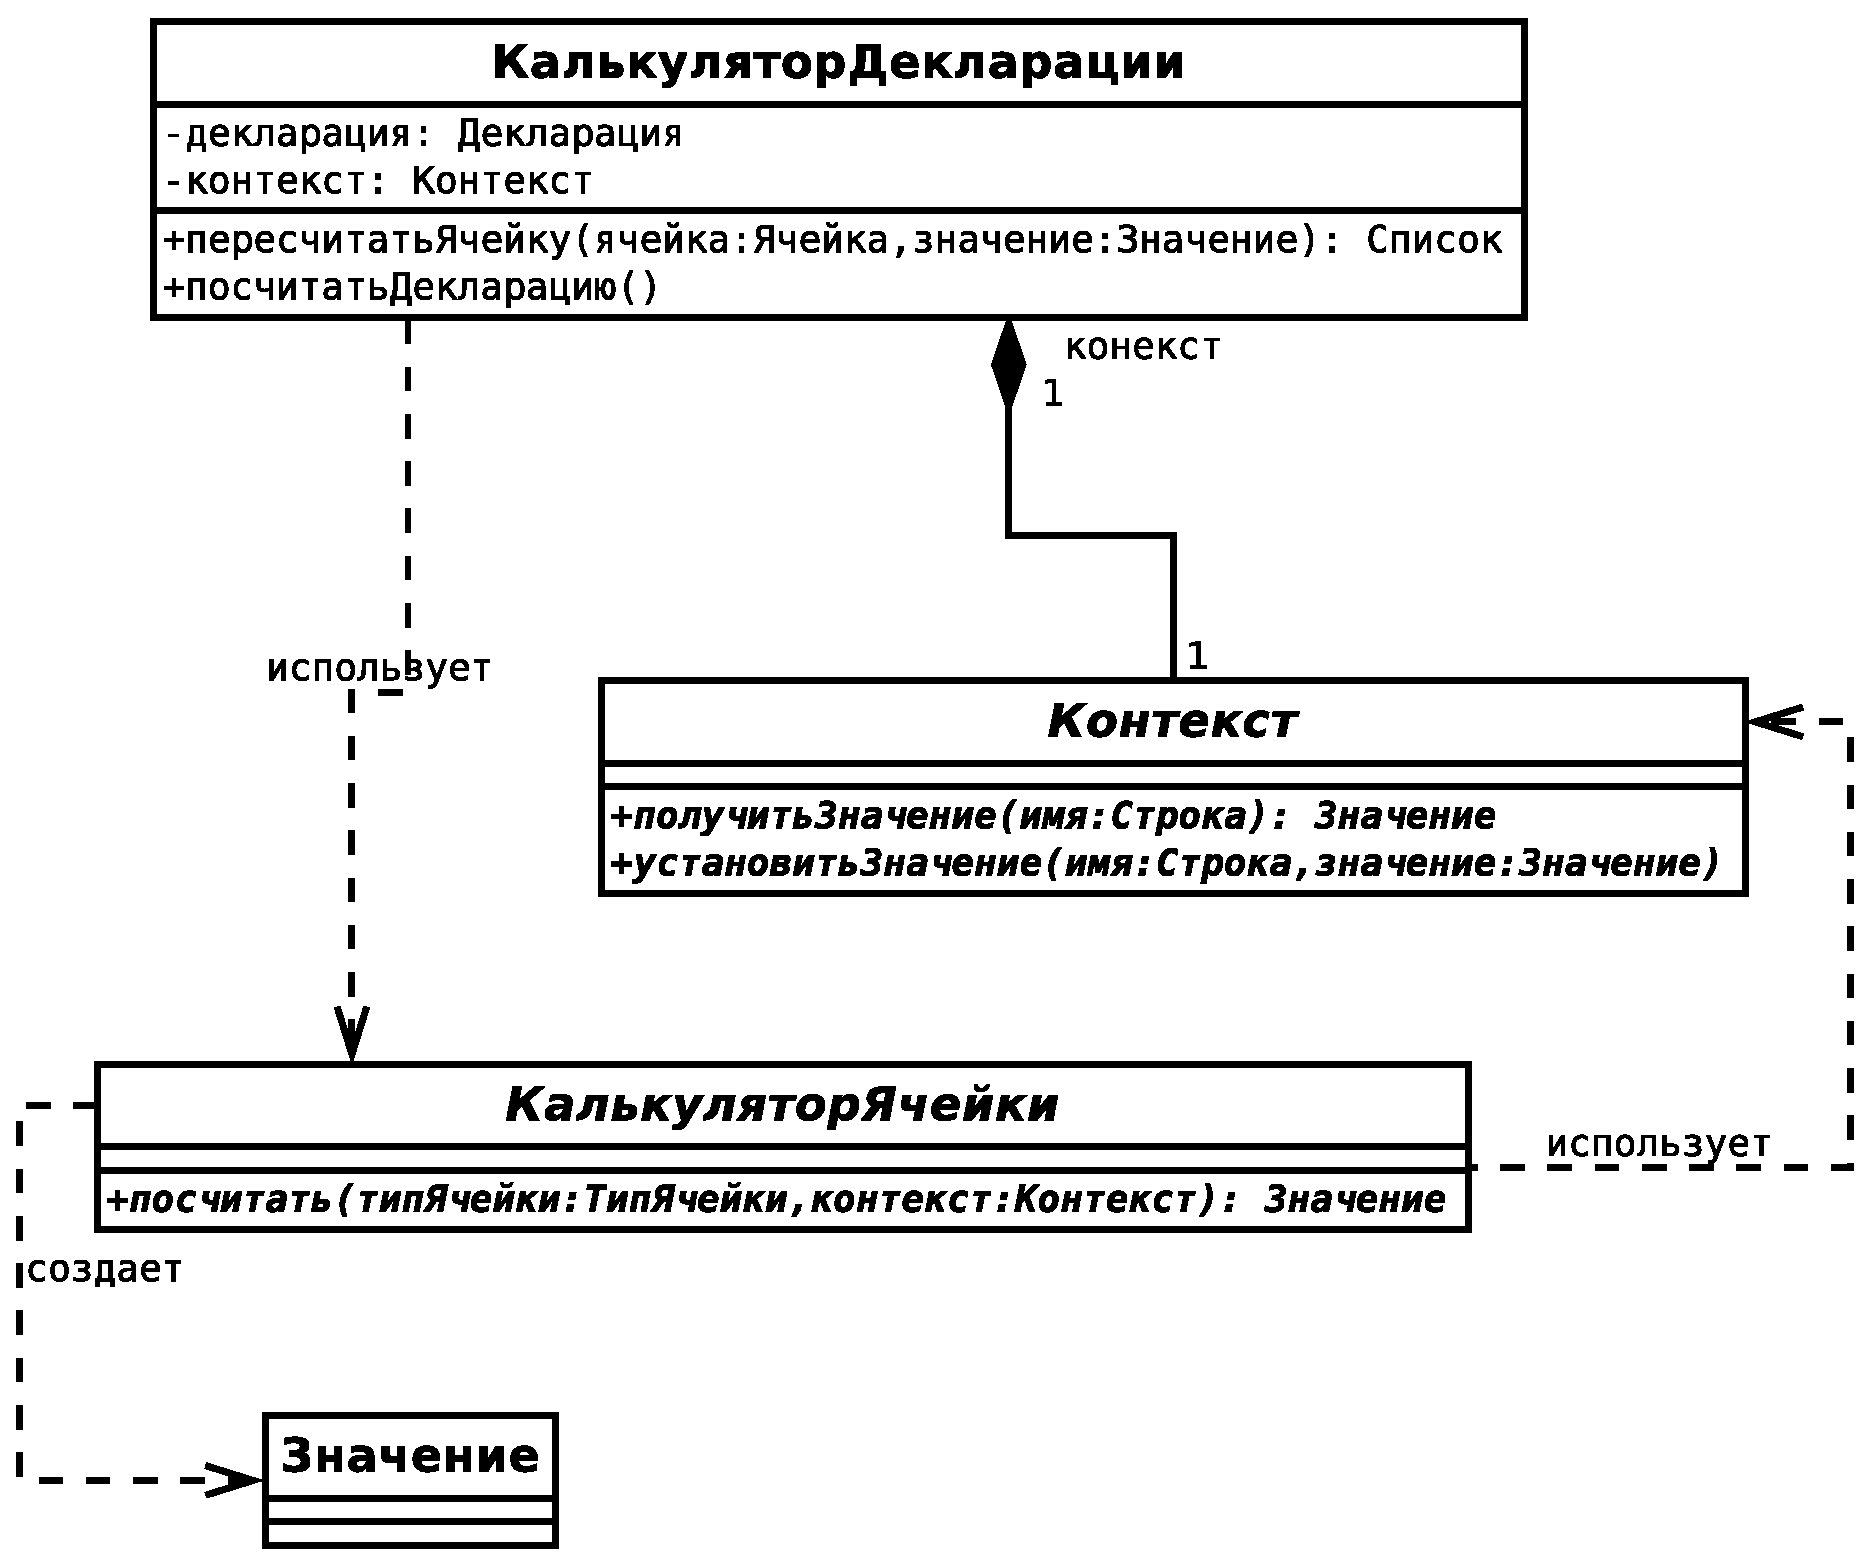
\includegraphics[scale=0.4]{uml/_classes_3}
  \caption{Диаграмма объектов, участвующих в подсчете декларации}
  \label{pic:classes_3}
\end{figure}

Подробнее рассмотрим объекты, участвующие в подсчете ячейки (рисунок \ref{pic:classes_2}). Объекты ``Пользовательская'', ``Счета'' и ``Формула'' расширяют объект ``ТипЯчейки'', представляя соответственно пользовательский, счета и формульный тип ячеек. Тип ``Счета'' содержит атрибут ``интервалы'', который представляет собой список интервалов для подсчета ячейки. Объект ``КалькуляторСчетовойЯчейки'', ``КалькуляторФормульнойЯчейки'' и ``КалькуляторПользовательскойЯчейки'' реализуют абстрактный метод ``посчитать'' объекта ``КалькуляторЯчейки'' для подсчета ячеек разных типов (счета, формульная и пользовательская). ``КалькуляторСчетовойЯчейки'' использует ``БухгалтерскуюКнигу'' для подсчета ячейки, так как подсчет интервалов использует ``Счета'', лежащие в данном интервале.

\begin{sidewaysfigure}
  \centering
  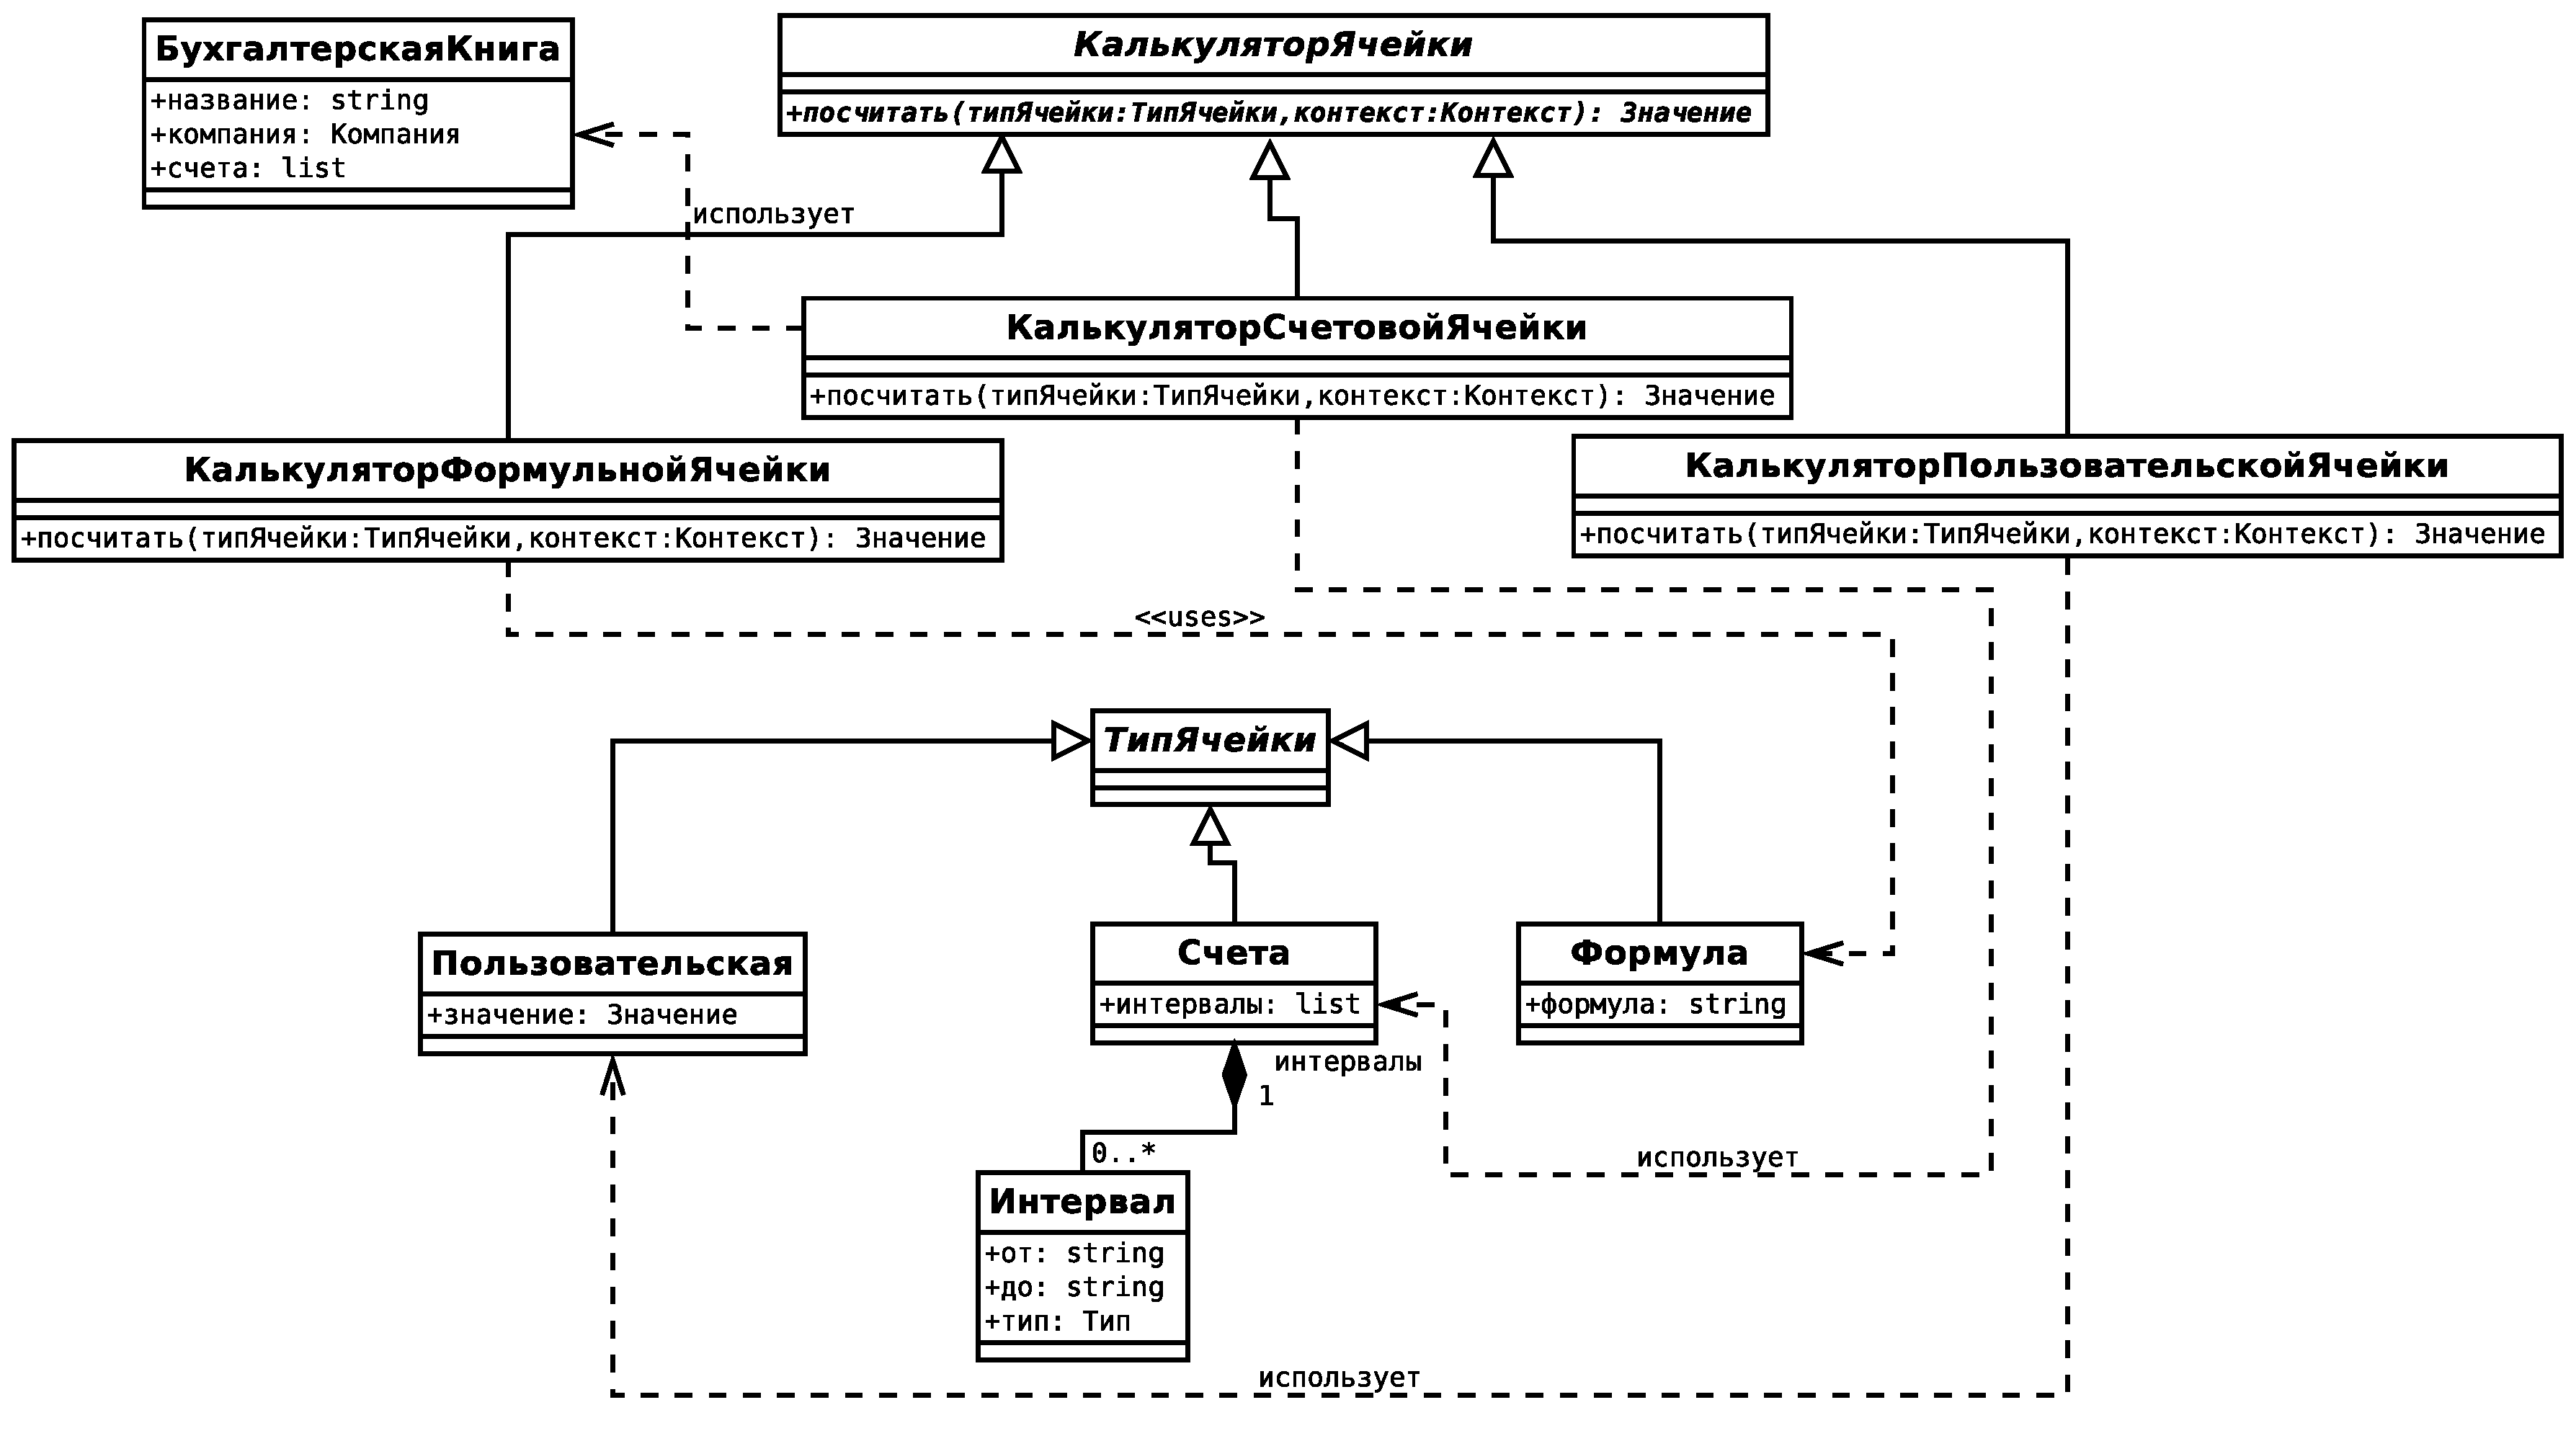
\includegraphics[scale=0.4]{uml/_classes_2}
  \caption{Диаграмма объектов, участвующих в подсчете ячейки}
  \label{pic:classes_2}
\end{sidewaysfigure}

Рассмотрим объект ``КалькуляторФормульнойЯчейки'' (рисунок~\ref{pic:classes_4}). Данный объект подсчитывает значение формульного типа ячейки, согласно атрибуту ``формула'' объекта ``Формула''. Значение атрибута является выражением на формальном языке. Опишем грамматику данного языка:

\begin{verbatim}
 number = integer | double
 simple_expr = number | str_const | variable
          | func_call | '('  expression  ')'
 unary_op = "-" | "!"
 bin_op = "<" | ">" | "<=" | ">="
          | "+" | "-" | "*" | "/" | "&"
          | "&&" | "||" | "^"
 expression = (simple_expr | un_op expression)
         ( bin_op  expression )*
 func_call = ident '(' (params){0,1} ')'
 params = expression | expression ',' params
\end{verbatim}

Типы данных:
\begin{itemize}
  \itemцелое(integer);
  \itemвещественное(double);
  \itemстроковая константа (ограничена с обеих сторон ');
  \itemарифметические операции: +, -, *, /;
  \itemлогические операции: \&\&, ||, !, <, >, <=, >=;
  \itemконкатенация строк - оператор \&;
  \itemпеременные: набор символов между ``\$\{`` слева и ``\}'' справа;
  \itemвызов функции: имя\_функции(параметры...)
\end{itemize}

Возвращаемое значение может быть четырех типов: строковое, целое, вещественное, булево (true или false).

\begin{figure}
  \centering
  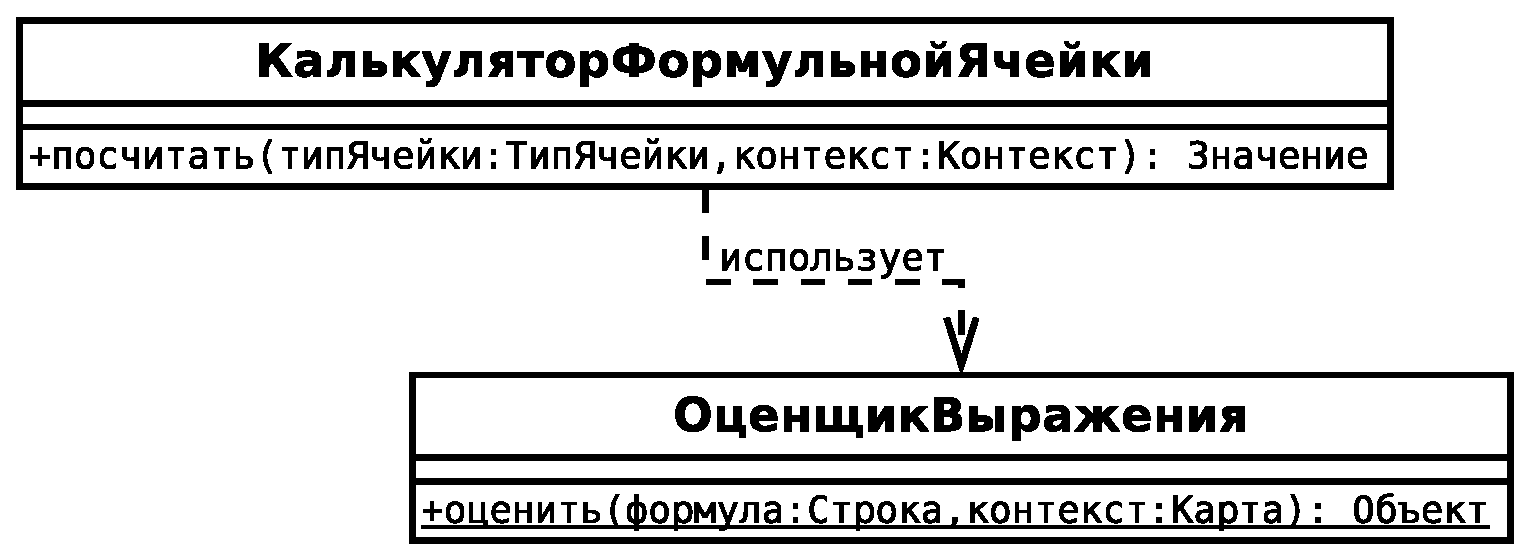
\includegraphics[scale=0.4]{uml/_classes_4}
  \caption{Диаграмма объектов, участвующих в подсчете формульной ячейки}
  \label{pic:classes_4}
\end{figure}

\section{Представление декларации в формате XML}
Для физического представления декларации был выбран язык XML. XML — это иерархическая структура, предназначенная для хранения любых данных. Визуально структура может быть представлена как дерево. Важнейшее обязательное синтаксическое требование заключается в том, что документ имеет только один корневой элемент. Это означает, что текст или другие данные всего документа должны быть расположены между единственным начальным корневым тегом и соответствующим ему конечным тегом.

Для описания структуры декларации необходимо описать свойства объектов: ``Декларация'', ``Ячейка'', свойство ``ТипыЯчеек'' (что является списком, который содержит объекты типа ``ТипЯчейки'') объекта ``СостояниеЯчейки''. Свойства ``Декларации'' возможно выделить в иерархическую структуру (рисунок~\ref{pic:xmlrepresentation}).

\begin{figure}
  \centering
  \includegraphics[scale=0.5]{uml/xmlrepresentation}
  \caption{Структура XML документа, представляющего структуру декларации}
  \label{pic:xmlrepresentation}
\end{figure}

\section{Логическая модель базы данных}
Представим логическую модель базы данных (рисунок~\ref{pic:domain_model}). На диаграмме отображены объекты, которые будут храниться в базе данных и отношения между ними. Объект ``Компания'' может иметь ``НалоговыеФормы'' и ``БухлалтерскиеКниги''. ``БухгалтерскаяКнига'' может содержать ``Счета''. ``НалоговыеФормы'' могут содержать ``СостоянияДекларации''. ``СостояниеДекларации'' сожержит ``СостояниеЯчеек''. Объект ``СостояниеЯчейки'' содержит ``Значение'' и текущий ``ТипЯчейки''. ``ТипЯчейки'' может быть ``Счета'', ``Пользовательская'' и ``Формула'' (на диаграмме данное отношение изображено как наследование). Тип ячейки ``Счета'' содержит ``Интервалы''.

\begin{figure}
  \centering
  \includegraphics[scale=0.4]{uml/domainmodel}
  \caption{Логическая модель данных}
  \label{pic:domain_model}
\end{figure}

\chapter{Реализация системы создания и управления электронными налоговыми декларациями}

\section{Выбор и обоснование средств разработки}
Для реализации системы документооборота использовался язык программирования Java. Java - объектно-ориентированный язык программирования, разрабатываемый компанией Sun Microsystems.Программы на Java транслируются в байт-код, выполняемый виртуальной машиной Java (JVM) — программой, обрабатывающей байтовый код и передающей инструкции оборудованию как интерпретатор, но с тем отличием, что байтовый код, в отличие от текста, обрабатывается значительно быстрее.
Достоинство подобного способа выполнения программ — в полной независимости байт-кода от операционной системы и оборудования, что позволяет выполнять Java-приложения на любом устройстве, для которого существует соответствующая виртуальная машина. Другой важной особенностью технологии Java является гибкая система безопасности благодаря тому, что исполнение программы полностью контролируется виртуальной машиной. Любые операции, которые превышают установленные полномочия программы (например, попытка несанкционированного доступа к данным или соединения с другим компьютером) вызывают немедленное прерывание.
Особенности языка:
\begin{itemize}
  \item автоматическое управление памятью
  \item расширенные возможности обработки исключительных ситуаций
  \item богатый набор средств фильтрации ввода/вывода
  \item набор стандартных коллекций, таких как массив, список, стек и т.д.
  \item наличие простых средств создания сетевых приложений (в том числе с использованием протокола RMI)
  \item наличие классов, позволяющих выполнять HTTP-запросы и обрабатывать ответы
  \item встроенные в язык средства создания много-поточных приложений
\end{itemize}
Следует отметить, что для данного языка существует большое количество библиотек, распространяемых под свободными лицензиями, для работы с различными форматами файлов, работы с базами данных, для разработки пользовательских интерфейсов, написания приложений, использующих веб-интерфейс и т.д.

\section{Выбор инструментальных средств разработки}

\subsection{Фреймворк Spring}
Фреймворк Spring - open source фреймворк для Java-платформы. Первая версия была написана Родом Джонсоном, который впервые опубликовал её вместе с изданием своей книги ``Expert One-on-One Java EE Design and Development''
Фреймворк был впервые выпущен под лицензией Apache 2.0 license в июне 2003 года. Первый стабильный релиз 1.0 был выпущен в марте 2004. Последующие стабильные релизы вышли в сентябре 2004 года и марте 2005 года.
Несмотря на то, что Spring Framework не обеспечивал какую-либо конкретную модель программирования, он стал широко распространённым в Java сообществе главным образом как альтернатива и замена модели Enterprise JavaBeans. Spring Framework предоставляет большую свободу Java разработчикам в проектировании, кроме того, он предоставляет хорошо документированные и лёгкие в использовании решения проблем, возникающих при создании приложений промышленного масштаба.
Между тем, особенности ядра Spring Framework применимы в любом Java приложении, и существует множество расширений и усовершенствований для построения веб-приложений на Java Enterprise платформе. По этим причинам Spring приобрёл большую популярность и признаётся разработчиками как стратегически важный фреймворк.
(Аннотация: диаграмма модулей Spring Framework и перечисление используемых модулей SF в системе)

\subsection{Библиотека Hibernate}
Библиотека Hibernate — библиотека для языка программирования Java, предназначенная для решения задач объектно-реляционного проецирования (object-relational mapping — ORM). Она представляет собой свободное программное обеспечение с открытым исходным кодом , распространяемое на условиях GNU Lesser General Public License. Данная библиотека предоставляет лёгкий в использовании каркас (фреймворк) для отображения объектно-ориентированной модели данных в традиционные реляционные базы данных.
Целью Hibernate является освобождение разработчика от значительного объёма сравнительно низкоуровневого программирования по обеспечению хранения объектов в реляционной базе данных. Разработчик может использовать Hibernate как в процессе проектирования системы классов и таблиц ``с нуля'', так и для работы с уже существующей базой данных.
Hibernate не только решает задачу связи классов Java с таблицами базы данных (и типов данных Java с типами данных SQL), но также предоставляет средства для автоматической генерации и обновления набора таблиц, построения запросов и обработки полученных данных и может значительно уменьшить время разработки, которое обычно тратится на ручное написание SQL- и JDBC-кода. Hibernate автоматизирует генерацию SQL-запросов и освобождает разработчика от ручной обработки результирующего набора данных и преобразования объектов, максимально облегчая перенос (портирование) приложения на любые базы данных SQL.
Hibernate обеспечивает прозрачную поддержку сохранности данных  для ``POJO'' (то есть для стандартных Java-объектов). единственное строгое требование для сохраняемого класса — наличие конструктора по умолчанию (без параметров).
Hibernate используется как в standalone Java-приложениях, так и в приложениях на платформе Java EE, использующих сервлеты или EJB.

\section{Программная реализация компонентов системы}

В результате выполнения проекта была разработана система создания и управления электронными налоговыми декларациями. Диаграмма компонентов системы представлена на рисунке~\ref{pic:componentsdiagram}. Было реализовано шесть компонентов:
\begin{itemize}
  \itemПодсистема управления декларацией - подсистема представляет собой набор классов для управление декларацией, что включает в себя загрузку структуры декларации, подсчет декларации, пересчет отдельных ячеек декларации.
  \itemПодсистема вычисления выражений - набор классов, которые осуществляют подсчет выражения на формальном языке, данная подсистема используется подсистемой управления декларацией для подсчета формульного типа ячеек
  \itemПодсистема управления - подсистема управляет остальными подсистемами
  \itemПодсистема хранения - подсистема, предоставляющая возможность сохранения, загрузки и обновления объектов, которые находятся в базе данных, для реализации данной подсистемы использовалась библиотека Hibernate
  \itemПодсистема отображения - подсистема, предоставляющая пользователю интерфейс для взаимодействия с системой.
  \itemМодель - содержит классы, представляющие собой сущности предметной области, такие как ``Компания'', ``Налоговые Формы'', ``Бухгалтерская Книга'', ``Счет'', ``Ячейка'' и т.д.
\end{itemize}

\begin{figure}
  \centering
  \includegraphics[scale=0.4]{uml/componentsdiagram}
  \caption{Диаграмма компонентов системы}
  \label{pic:componentsdiagram}
\end{figure}

\subsection{Реализация модельных классов}
На рисунке~\ref{pic:model_classes} приведены модельные классы и отношения между ними. Рассмотрим данные классы в контексте выделенных на этапе проектирования объектов.
\begin{itemize}
  \item Cell - представляет ячейку, имеет атрибуты: ``name''- имя ячейки, ``state'' -состояние ячейки, ``valueType'' - тип зачения;
  \item CellState - представляет состояние ячейки, имеет атрибуты: ``types'' - список возможны типов ячейки (экземпляры класса CellType), ``cellValue'' - значение, ``activeType'' - текущий тип ячейки. Атрибут ``name'' (имя) был введен, так как данный объект будет отражен на соответсвующую таблицу в базе данных, при отображений из записи в таблице базы данных на данный объект необходимо его сопоставить с соответствующим экземпляром класса ``Cell''. Атрибут ``id'' является уникальным идентификатором;
  \item CellValue - представляет значение ячейки, имеет атрибуты: ``id'' - уникальный идентификатор, ``doubleValue'' - вещественное значение,\\ ``longValue'' - целочисленное значение, ``stringValue'' - строковое значение, ``valueType'' - тип хранимого значения (целочисленный, строковый либо вещественный);
  \item Report - представляет декларацию, содержит атрибуты: ``name'' - имя декларации, ``Cell'' - множество ячеек, ``crossReports'' - список деклараций, от которых зависит значения ячеек данной декларации (в формульной ячейке может использоваться переменная, которая содержит значение ячейки из другой декларации), ``reportState'' - состояние декларации;
  \item ReportState - представляет состояние декларации. Содержит атрибуты: ``id'' - уникальный идентификатор;
  \item CellType - абстрактный класс, представляет тип ячейки;
  \item CellTypeAccounts - расширяет класс CellType, представляет собой тип ячейки ``Счета'';
  \item CellTypeEditable - расширяет класс CellType, представляет собой тип ячейки ``Пользовательская'';
  \item CellTypeFormula - расширяет класс CellType, представляет собой тип ячейки ``Формула'';
  \item Account - представляет интервал, атрибуты: ``accFrom'' - начало интервала, ``accTo'' - конец интервала, ``sign'' - знак (``+'' либо ``-''), ``type'' - тип (дебет либо кредит);
  \item Company - представляет компанию, параметры: ``id'' - уникальный идентификатор, ``name'' - название компании, ``code'' - код компании;
  \item TaxKit - представляет налоговые формы, ``id'' - уникальный идентификатор, ``name'' - имя, ``selected'' - показыват выбраны ли данные налоговые формы в качестве текущих, ``ledger'' - бухгалтерская книга, счета которой будут использоваться для подсчета соответствующих ячеек деклараций, ``company'' - компания, которой принадлежат данные налоговые формы
  \item Ledger - представляет бухгалтерскую книгу, ``id'' - уникальный идентификатор, ``name'' - имя, ``company'' - компания, которой принадлежит бухгалтерская книга, ``accounts'' - список счетов, принадлежащих бухгалтерской книге;
  \item LedgerAccount - представляет запись в бухгалтерской книге (``Счет''), ``debit'' - значение дебета для счета, ``credit'' - значение кредита для счета, ``number'' - номер счета;
\end{itemize}

\begin{sidewaysfigure}
  \centering
  \includegraphics[scale=0.4]{uml/impl_model}
  \caption{Диаграмма модельных классов}
  \label{pic:model_classes}
\end{sidewaysfigure}

\subsection{Реализация подсистемы управления декларацией}

На рисунке~\ref{pic:loadclasses} изображена диаграмма классов для загрузки декларации.

\begin{figure}
  \centering
  \includegraphics[scale=0.35]{uml/impl_classes1}
  \caption{Диаграмма классов для загрузки декларации}
  \label{pic:loadclasses}
\end{figure}

На рисунке~\ref{pic:reportmanager} изображена диаграмма классов, участвующих в управлении декларацией.

\begin{sidewaysfigure}
  \centering
  \includegraphics[scale=0.4]{uml/impl_classes2}
  \caption{Диаграмма классов для управления декларацией}
  \label{pic:reportmanager}
\end{sidewaysfigure}

\subsection{Реализация подсистемы вычисления выражений}

Выражение представляет собой выражение на формальном языке. Для вычисления значения выражения используется схема, приведенная на рисунке~\ref{pic:evalprocess}. Лексический анализатор анализирует входную строку (выражение) и представляет его в виде последовательности лексем.

\begin{figure}
  \centering
  \includegraphics[scale=0.4]{uml/eval_algorithm}
  \caption{Процесс вычисления значения выражения}
  \label{pic:evalprocess}
\end{figure}

Были выделены следующие лексемы:

\begin{itemize}
  \itemЦелое число(INTEGER);
  \itemВещественное число (DOUBLE);
  \itemСтрока (STRING);
  \itemРазделитель (DELIMETER);
  \itemПеременная (VARIABLE);
  \itemИдентификатор (IDENTIFIER);
  \itemКонец выражения (EOF);
\end{itemize}

Далее лексемы обрабатываются синтаксическим анализатором, который создает абстрактное синтаксическое дерево, у каждого узла дерева могут быть потомки, были выделены следующие узлы:
\begin{itemize}
  \itemБинарная операция (BinOp);
  \itemВызов функции (FuncCallAST);
  \itemПараметр функции (FuncParamAST);
  \itemЛитерал (LiteralAST);
  \itemЧисло (NumberAST);
  \itemУнарная операция (UnaryOpAST);
  \itemПеременная (VariableAST);
\end{itemize}

После того, как абстрактное синтаксическое дерево создано, интерпретатор обрабатывает дерево, после чего получается результат вычисления выражения. Представим классы, которые вычисляют выражение, на рисунке~\ref{pic:evalclasses}.

\begin{sidewaysfigure}
  \centering
  \includegraphics[scale=0.4]{uml/impl_classes3}
  \caption{Диаграмма классов для вычисления значения выражения}
  \label{pic:evalclasses}
\end{sidewaysfigure}

\subsection{Реализация подсистемы управления}

Классы подсистемы управления занимаются обработкой запросов и предоставляют взаимодействие остальных подсистем. Для обработки запросов используется модуль фреймворка Spring, Spring MVC. Для обработки запросов Spring MVC использует сервлет ``DispatcherServlet'' который делегирует запросы контроллерам. Контроллеры должны реализовывать методы для обработки запросов. Методы, обрабатывающие запросы возвращают название представления, которое необходимо вернуть клиенту. В качестве представления используется JSP(Java Servler Pages). В качестве ответа на запрос вместе с представлением могут возвращаться модельные данные, например список, состоящий из экзепляров класса, который затем будет обработан JSP страницей.
В случае обработки асинхронных запросов, методы должны возвращать данные, которые будут переданы клиенту.

В подсистеме управления реализованы следующие контроллеры:
\begin{itemize}
  \item CompanyController - содержит методы для обработки запросов на отображение списка доступных компаний, для отображения компании, метод для удаления компании. Метод для отображения списка компаний в качестве модельных данных возвращает список объектов ``Company'', которые загружаются из базы данных с использованием подсистемы хранения. Метод для отображения компании, в зависимости от параметра ``id'' запроса, посредством подсистемы хранения получает экземпляр класса ``Company'', который передается соответствующей JSP странице для отображения;
  \item LedgerController - содержит методы для обработки запросов на отображения списка доступных бухгалтерских книг, для отображения свойств конкретной бухгалтерской книги, для отображения формы редактирования бухгалтерской книги, для создания бухгалтерской книги;
  \item ReportController - содержит метод для обработки запросов на отображение декларации. При обработке запроса на отображение декларации, посредством подсистемы управления декларацией, создает нужную декларацию и передает структуру декларации подсистеме отображения;
  \item ReportStateController - содержит методы для обработки запросов на получения состояния ячеек декларации, на пересчет ячейки и зависимых ячеек, на изменение типа ячейки, на сохранение состояния декларации. Для получения состояния ячеек используется подсистема хранения, посредством которой получается сохраненный объект ``ReportState''. Для получения объекта ``ReportState'' необходимы идентификатор выбранных налоговых форм и название текущей декларации, данные параметры должны находиться в запросе;
  \item TaxKitController - содержит методы для отображения списка налоговых форм (``TaxKit''), для удаления наловых форм. Данные действия производятся посредством подсистемы хранения;
  \item TaxKitCreateController - содержит методы для создания налоговых форм. Метод для обработки запроса на отображения формы создания налоговых форм возвращает название соответствующей страницы. Метод для обработки запроса на добавления налоговых форм, на основании параметров, переданных формой создания создает новые налоговые формы.
  \item TaxKitEditController - содердит методы для редактирования налоговых форм. Метод для обработки запросы на отображение формы редактирования возвращает название соответствующей страницы, в качестве модельных данных возвращает экземпляр налоговых форм, который был получен посредством подсистемы хранения.
\end{itemize}

\subsection{Реализация подсистемы хранения}

Подсистема хранения используется для добавления, получения и удаления сущностей системы из базы данных. На таблицы в базе данных отображаются следующие классы: ``ReportState'', ``CellState'', ``CellTypeFormula'',\\``CellTypeAccounts'', ``CellTypeEditable'', ``Account'', ``CellValue'', ``TaxKit'',\\``Company'', ``Ledger'', ``LedgerAccount''. Данная подсистема была реализована с использованием библиотеки Hibernate. Каждый объект был отображен на соответствующую таблицу в базе данных, так же отображены связи между объектами. Примитивные типы данных Java отображаются на типы данных SQL.

На рисунке~\ref{pic:ormsample} рассмотрим отображение объектов ``ReportState'' и\\ ``CellState'' на таблицы в базе данных. Класс ``ReportState'' отображен на таблицу ``REPORTSTATE'', атрибут ``id'' класса ``ReportState'' отображен в соответствующий атрибут таблицы и является первичным ключом. Класс ``CellState'' отображен на таблицу ``CELLSTATE'', у данной таблицы есть атрибут ``REPORTSTATE\_ID'' который является внешним ключом, ссылающимся на атрибут ``ID'' таблицы ``REPORTSTATE'' данная ссылка отображает отношение ``ReportState'' к ``CellState'' как 1:n.

\begin{figure}
  \centering
  \includegraphics[scale=0.4]{uml/ormsample}
  \caption{Отображение классов ``ReportState'', ``CellState'' и связи между ними на таблицы в базе данных}
  \label{pic:ormsample}
\end{figure}


\subsection{Реализация подсистемы отображения}



\subsection{Физическая модель базы данных}
Представим физическую модель базы данных(рисунок~\ref{pic:database}, которая была построена на основании логической модели.
\begin{figure}
  \centering
  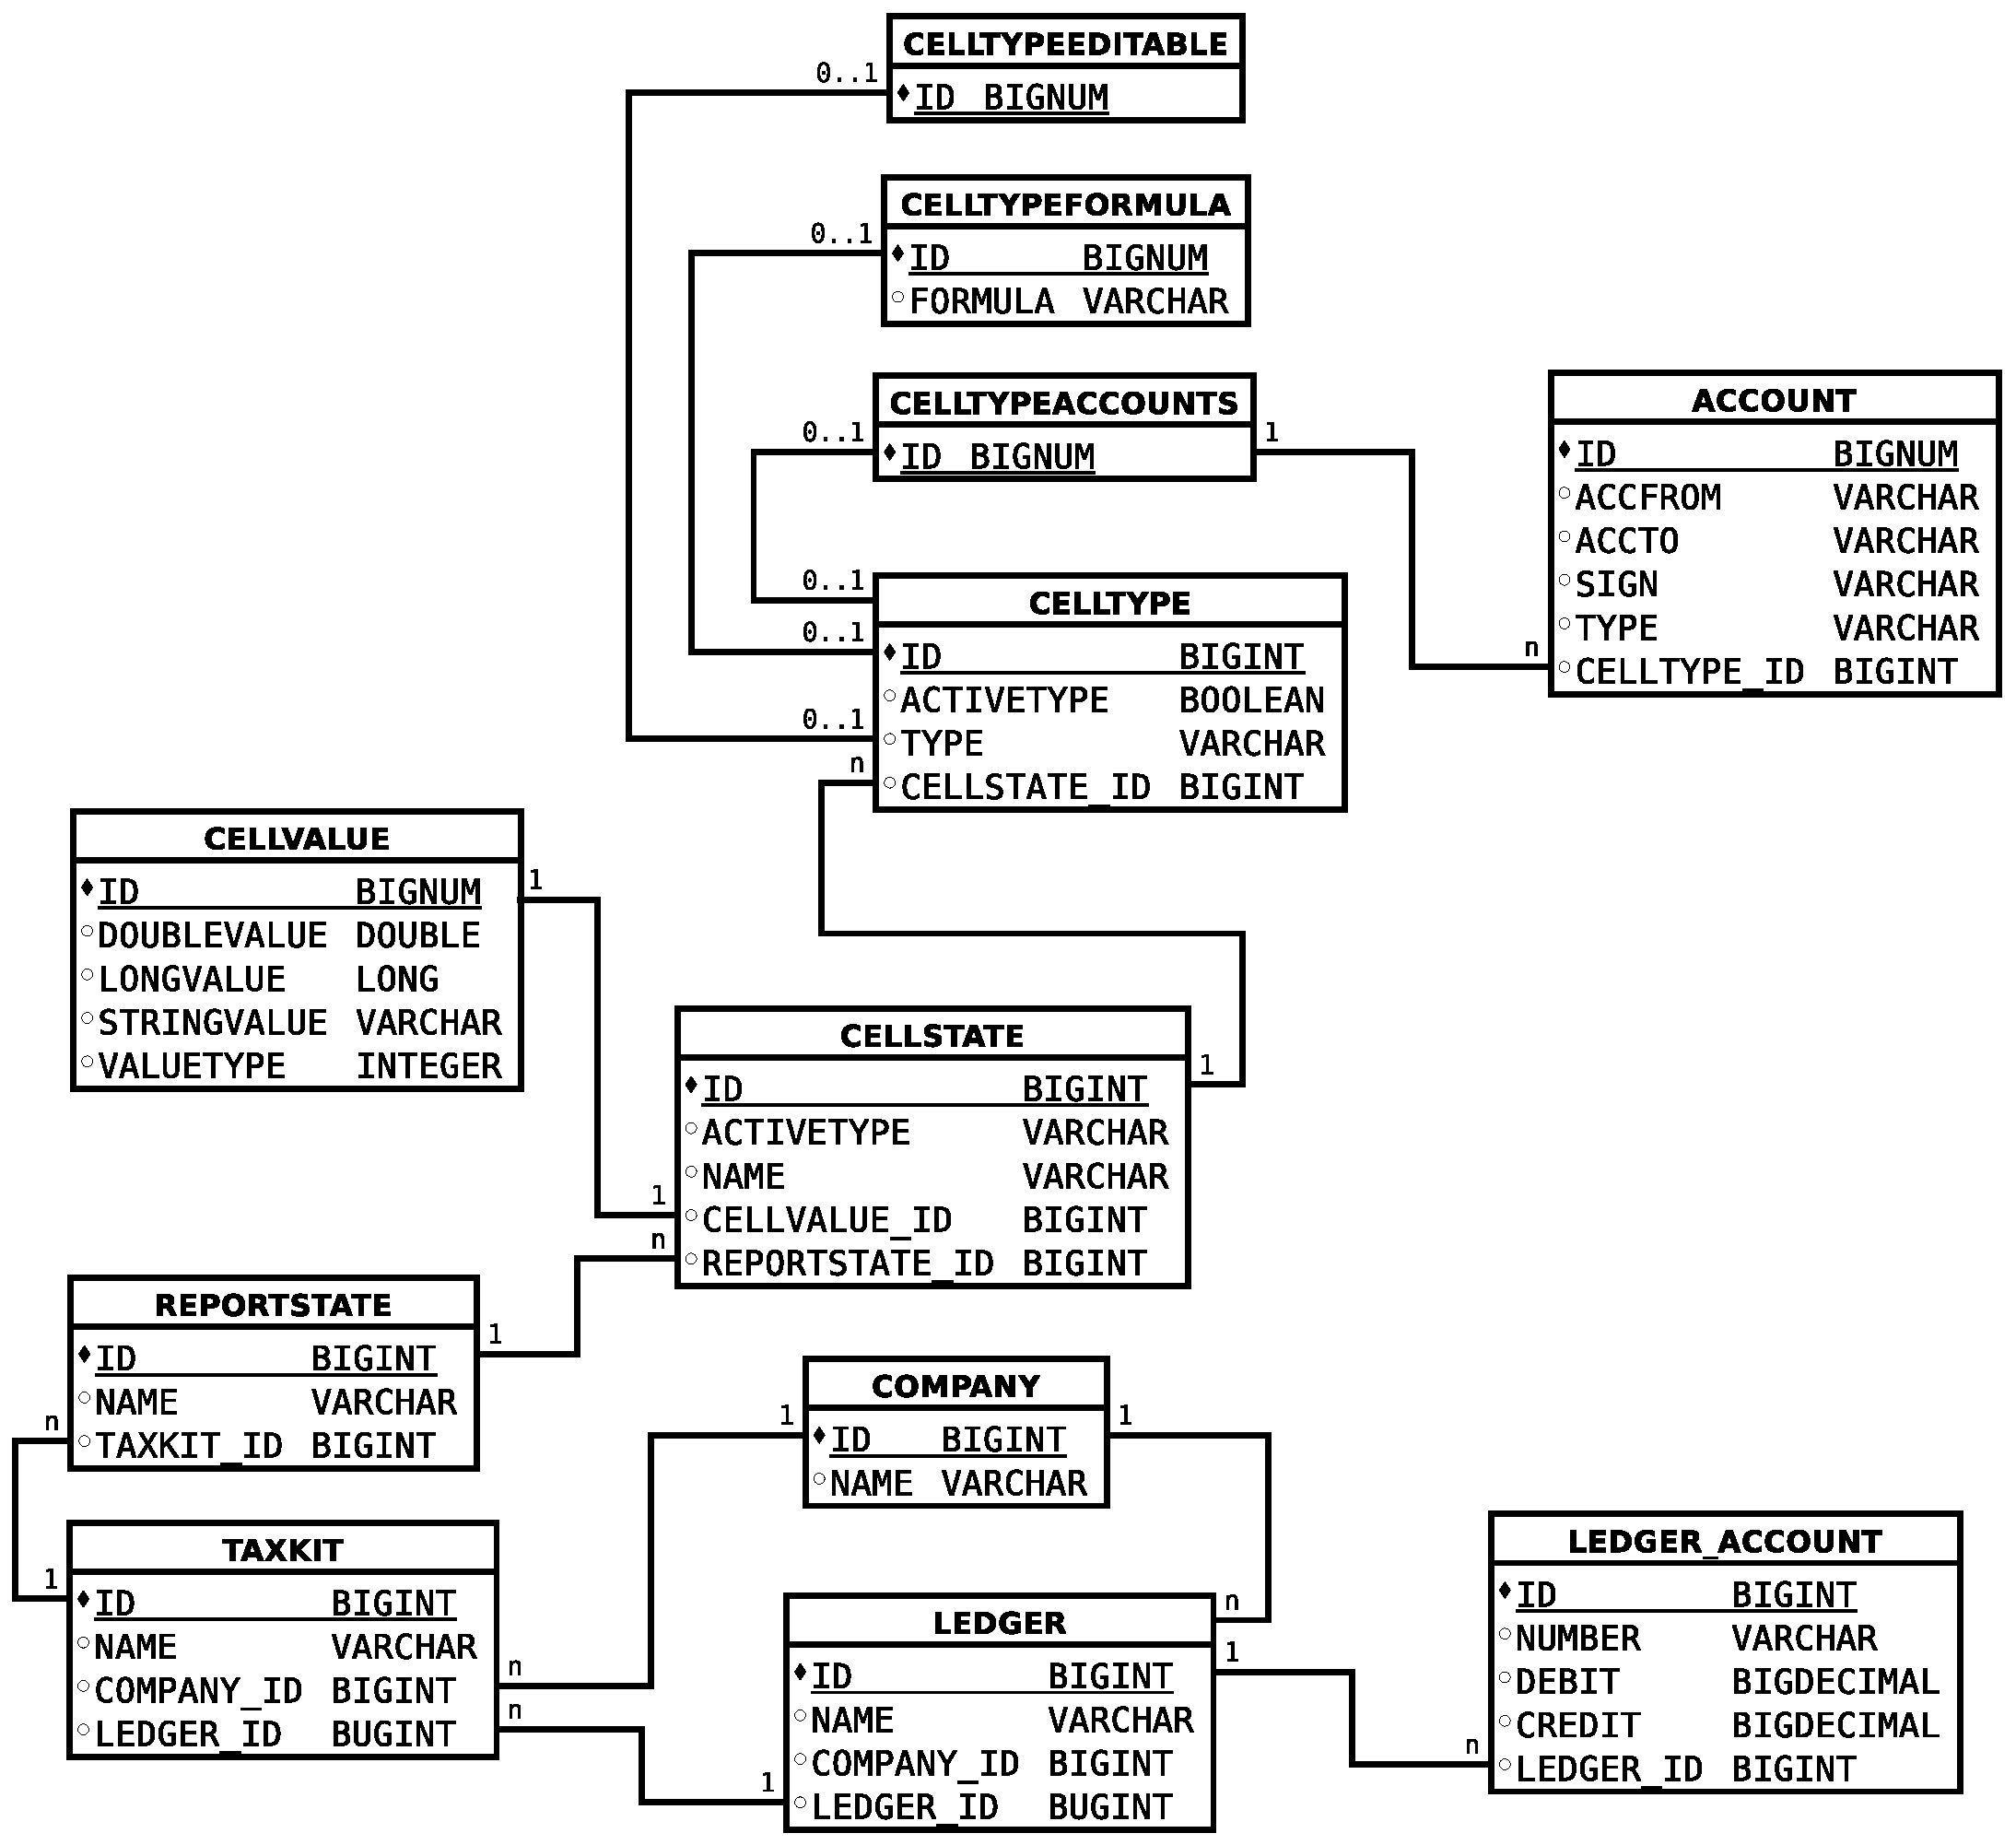
\includegraphics[scale=0.4]{uml/database}
  \caption{Схема базы данных}
  \label{pic:database}
\end{figure}

\section{Тестирование}
В целях тестирования кода и контроля качества во время разработки были написаны модульные тесты. Тесты представляют собой набор утверждений, которые не должны быть опровергнуты в результате ожидаемой (корректной) работы тестируемого модуля. В данном контексте модулем является тестируемый класс. Наборы утверждений объединяются в методах. В рамках соглашения был использован следующий формат имени метода: ``testMethod'', где Method - название тестируемого метода.
Ниже приведен список классов, для которых были написаны модульные тесты:
\begin{itemize}
  \item XMLCellLoader
  \item XMLReportLoader
  \item ReportFactoryImpl
  \item ReportInterpreter
  \item ReportManager
  \item ReflectionAssembler
  \item XMLFileReader
  \item ReportStateController
  \item TaxKitReportStateDAOImpl
  \item ReportsServiceImpl
\end{itemize}

\chapter*{Охрана труда и экологическая безопасность}
\addcontentsline{toc}{chapter}{Охрана труда и экологическая безопасность}
Обеспечение комфортных условий труда разработчиков систем электронного документооборота


\chapter*{Технико-экономическое обоснование}
\addcontentsline{toc}{chapter}{Технико-экономическое обоснование}
(Технико-экономическое обоснование системы учета и управления электронными налоговыми декларациями)


\begin{thebibliography}{99}
\addcontentsline{tok}{chapter}{Список литературы}
\bibitem{refwikidoc} Система автоматизации документооборота [Электронный ресурс] / Сообщество wikipedia, 2010. -- Режим доступа: http://ru.wikipedia.org/wiki/Система\_автоматизации\_документооборота -- Дата доступа 19.03.2010
\bibitem{refdoconline} Документооборот и делопроизводство. Системы электронного документооборота. [Электронный ресурс] . -- Режим доступа: http://www.doc-online.ru -- Дата доступа 19.03.2010
\bibitem{refwikixml} XML [Электронный ресурс] / Сообщество wikipedia, 2010. -- Режим доступа: http://ru.wikipedia.org/wiki/XML -- Дата доступа 19.03.2010
\bibitem{refspecxml} Extensible Markup Language (XML) 1.0 (Fifth Edition) [Электронный ресурс] / W3C. -- Режим доступа: Extensible Markup Language (XML) 1.0 (Fifth Edition) -- Дата доступа 19.03.2010
\bibitem{refelectrtaxesby} Государственная Целевая Программа по разработке программно-технического комплекса по автоматизации процесса расчета подлежащих уплате в бюджет сумм налогов, сборов (пошлин) и представлению в налоговые органы налоговых деклараций (расчетов) в электронном виде на 2008 - 2010 годы [Электронный ресурс] : Аппарат Совета Министров Республики Беларусь. -- Режим доступа : http://www.government.by/ public/ shared/ rus/ solutions /rus\_solution101170\_1.pdf -- Дата доступа 19.03.2010
\bibitem{refwikitaxreturn} Налоговая декларация [Электронный ресурс] / Сообщество wikipedia, 2010. -- Режим доступа: http://ru.wikipedia.org/wiki/Налоговая\_декларация -- Дата доступа 19.03.2010

\end{thebibliography}

\end{document}
